% LaTeX source for ``Algorithms for Computer Simulation of Molecular Systems''
% Copyright (c) 2023 รังสิมันต์ เกษแก้ว (Rangsiman Ketkaew).

% License: Creative Commons Attribution-NonCommercial-NoDerivatives 4.0 International (CC BY-NC-ND 4.0)
% https://creativecommons.org/licenses/by-nc-nd/4.0/

\chapter{การพัฒนาซอฟต์แวร์สำหรับเคมีเชิงคำนวณ}
\label{ch:software_dev}

%----------------------------------------
\section{การเขียนโปรแกรมทางเคมีเชิงคำนวณ}
%----------------------------------------

ถ้าหากผู้อ่านอยากจะศึกษาการเขียนโปรแกรมทางเคมีเชิงคำนวณจะเริ่มยังไงดี เช่น ต้องการเขียนโปรแกรม Density Functional Theory (DFT)
หรือ Implement วิธีโครงสร้างเชิงอิเล็กทรอนิกส์ (Electronic Structure) ผมขอให้ความเห็นอย่างนี้ครับว่าการจะที่เขียนโปรแกรมทางเคมี%
คำนวณขึ้นมาสักโปรแกรมหนึ่งนั้นใช้เวลามากพอสมควรเพราะว่ามีรายละเอียดที่ซับซ้อนมาก (เวลาที่ใช้ในการเขียนนั้นขึ้นอยู่กับว่าเขียนคนเดียวหรือช่วย%
กันเขียนหลายคน) ดังนั้นผมแนะนำว่าสำหรับผู้ที่เพิ่งเริ่มต้นการเขียนโปรแกรมทางวิทยาศาสตร์ควรศึกษาจากโปรแกรมมาตรฐานที่ได้รับความนิยมอยู่แล้ว
ผมไม่ได้บอกว่าห้ามเขียนโปรแกรมใหม่เองแบบเริ่มจากศูนย์หรือ From Scratch แต่ถ้าหากว่าเราเริ่มต้นเรียนรู้จากโปรแกรมที่ได้รับความนิยมและใช้งาน%
กันอย่างแพร่หลายอยู่แล้วก็มีข้อดีดังนี้

\begin{itemize}[topsep=0pt]
  \item ประหยัดเวลา ไม่ต้องมานั่งศึกษาหรือเขียนโค้ดใหม่เองทั้งหมด

  \item ได้เรียนรู้วิธีการเขียนโค้ดที่มีประสิทธิภาพจากนักพัฒนาคนอื่น ๆ

  \item เป็นการต่อยอดและพัฒนาโปรแกรมนั้น ๆ ให้ดีขึ้นไปอีกเพราะเราไม่จำเป็นต้องมา \enquote{Reinvent the Wheel}%
        \footnote{คือการพยายามทำสิ่งที่คนอื่นได้ทำเอาไว้ดีอยู่แล้วใหม่ตั้งแต่ต้น ซึ่งเป็นอะไรที่เสียเวลาและเสียทรัพยากรณ์ โดยไม่คุ้มค่าเอาเสียเลย}

  \item เป็นการสร้างเครือข่ายนักวิจัยและความร่วมมือทางวิชาการในระดับนานาชาติ
\end{itemize}

\noindent อย่างไรก็ตามถ้าหากใครอยากจะเริ่มเขียนโปรแกรมเองนั้น (ไม่จำเป็นต้องเป็น DFT อย่างเดียว แต่รวมถึงวิธีการจำลองทางคอมพิวเตอร์อื่น ๆ
ด้วย เช่น Molecular Dynamics หรือ Monte Carlo) ก็มีข้อดีหลายข้อเหมือนกัน ดังนี้

\begin{itemize}[topsep=0pt]
  \item ได้ทำความเข้าใจการเขียนโปรแกรมอ้างอิงตามสมการทาง Electronic Structure

  \item ฝึกทักษะการเขียนโปรแกรมสำหรับการคำนวณทางวิทยาศาสตร์และได้เรียนรู้เทคนิคการประมาณค่าเชิงตัวเลข

  \item ได้ออกแบบโปรแกรมเองและ Implement วิธีใหม่ ๆ ที่โปรแกรมอื่นไม่มี

  \item ต่อยอดเป็นโปรแกรมในรูปแบบเชิงพานิชย์ได้เพราะว่ามีโปรแกรมทางเคมีคำนวณหลาย ๆ โปรแกรมที่ขาย License
\end{itemize}

ประเด็นหรือคำถามสำคัญคือ \enquote{ถ้าหากอยากจะเริ่มศึกษาโค้ดของวิธีการคำนวณทางเคมีควอนตัม เช่น โปรแกรม Density Functional
  Theory (DFT) ดี ๆ สักตัวนึงจะเริ่มจากไหนดี?} ความเห็นของผมคือแนะนำให้ศึกษาโปรแกรม PySCF โดยมีเหตุผลดังต่อไปนี้

\begin{itemize}[topsep=0pt]
  \item โปรแกรมมีประสิทธิภาพสูง ทำงานได้เร็วและให้ผลการคำนวณที่ถูกต้องและแม่นยำและยังคำนวณได้หลากหลายวิธี

  \item มีผู้ใช้งานเยอะเนื่องจากว่าโปรแกรม PySCF นั้นสามารถติดตั้งและใช้งานได้ง่าย เตรียมไฟล์ Input ได้ไม่ยุ่งยาก

  \item PySCF เขียนด้วย Python เกือบทั้งหมด (87\% เขียนด้วย Python, 12\% เป็นภาษา C ก็คือพวกไลบรารี่ต่าง ๆ ที่เอามาคำนวณ%
        ในส่วนที่ Python อาจจะคำนวณได้ช้า) ดังนั้นจึงง่ายต่อการทำความเข้าใจ

  \item มีทีมพัฒนาที่ใหญ่และแข็งแกร่ง ได้รับการสนับสนุนฟีเจอร์และแก้ไข Bug อย่างต่อเนื่อง
\end{itemize}

\noindent จากข้อ 1 ถ้าหากเราต้องการ Implement วิธีหรือเทคนิคใหม่ ๆ เข้าไปใน PySCF ก็ทำได้ง่ายเพราะว่าเขียนด้วยภาษา Python
นอกจากนี้โปรแกรมยังสามารถทำงานด้วย GPU ได้ด้วย (มี Plugin พิเศษชื่อว่า gpu2pyscf) ตัวโค้ดถูกเขียนและได้รับการปรับปรุงมาเป็นอย่างดี
(Well-written) มีการวางโครงสร้างของโปรแกรมที่เรียบร้อย แบ่ง Methods ต่าง ๆ ออกเป็น Module ที่ชัดเจนและมีการจัดวาง Function
ที่เหมาะสม สำหรับผู้อ่านที่สนใจโปรแกรม PySCF ก็ไปดูได้ที่ \url{https://github.com/pyscf/pyscf}

เมื่อเราเลือกโปรแกรมได้แล้ว ขั้นตอนต่อมาก็คือพยายามทำความเข้าใจทฤษฎีของหัวข้องานวิจัยที่เราต้องการศึกษา พยายามหาว่าเราสามารถพัฒนา%
วิธีนั้น ๆ ได้อย่างไรเพื่อที่จะปรับปรุงให้มีความถูกต้องในการคำนวณมากขึ้นหรือหากรณีที่ทฤษฎีนั้นยังไม่ครอบคลุม ขั้นตอนต่อไปคือหาวิธีการแก้ไข%
ปัญหาหรือ Solution สำหรับการปรับปรุงทฤษฎีนั้นแล้วเขียนออกมาเป็นสมการทางคณิตศาสตร์ที่เราจะนำไป Implement ได้ ขั้นตอนต่อไปก็คือ%
การวางแผนการเขียนโปรแกรมซึ่งสามารถทำได้ด้วยการเขียนโค้ดเทียมหรือ Pseudo Code ก่อนที่เราจะ Implement จริง ๆ โดยเราจะต้องคิดเกี่ยว%
กับการวางโครงสร้างหรือ Structure ของโปรแกรม เช่น แบ่งโปรแกรมออกเป็นโปรแกรมย่อย ๆ หลายส่วน เช่น แบ่งเป็น modules, functions,
classes, หรือ types โดยเราควรจะต้องคำนึงถึงการพัฒนาโปรแกรมต่อไปในอนาคตด้วยว่าโปรแกรมของเรานั้นสามารถที่จะรองรับฟีเจอร์ใหม่ ๆ
ที่นักพัฒนาคนอื่น ๆ จะเข้ามาช่วยพัฒนาเพิ่มเติมได้

หลังจากที่เรา Implement เข้าไปในโปรแกรมเสร็จเรียบร้อยแล้วเราควรจะต้องมีการตรวจสอบการทำงานของโปรแกรมหรือฟังก์ชันต่าง ๆ อย่างสม่ำเสมอ%
เพื่อตรวจสอบค่าที่ได้จากคำนวณว่ามีความถูกต้องและมีความสมเหตุสมผลมากน้อยแค่ไหน เมื่อได้ค่าการคำนวณที่ถูกต้องแล้วขั้นตอนสุดท้ายก็คือการ%
ปรับปรุงหรือทำความสะอาดโค้ดให้มีประสิทธิภาพและอ่านได้ง่ายขึ้น ในขั้นตอนนี้เราสามารถเรียนรู้ได้จากการศึกษาโค้ดที่นักพัฒนาคนอื่นเขียนไว้ก็ได้%
ว่าเขาเขียนอย่างไร ใช้วิธีหรือเทคนิคอะไรที่ทำให้โค้ดรันได้เร็วและมีประสิทธิภาพ นอกจากนี้ยังมีสิ่งอื่น ๆ ที่เราควรจะต้องทำด้วย เช่น เขียน Comment
หรือทำเอกสารประกอบการใช้งาน (Documentation) เพื่อที่ว่าตัวเราเองหรือนักพัฒนาคนอื่น ๆ ที่มาอ่านหรือแก้ไขโค้ดของเรานั้นสามารถทำความ%
เข้าใจโค้ดได้ง่ายและไม่ต้องมานั่งศึกษาเองจากศูนย์

%----------------------------------------
\section{การวางโครงสร้างโปรแกรม}
%----------------------------------------

การที่เราจะเขียนโปรแกรมคำนวณทางวิทยาศาสตร์นั้นควรที่จะต้องมีการวางแผนให้ดีเพราะว่าเมื่อเราเขียนโค้ดไปเรื่อย ๆ ตัวโปรแกรมของเราก็จะมี%
ขนาดที่ใหญ่ขึ้นและมีความซับซ้อนมากขึ้นด้วย ดังนั้นการวางโครงสร้างของโปรแกรมเพื่อให้รองรับฟังก์ชันหรือฟีเจอร์ใหม่ ๆ ที่อาจจะมีการเขียนโค้ดเพิ่ม%
เข้ามานั้นช่วยให้โปรแกรมนั้นมีความเป็นระเบียบและง่ายต่อการ Maintenance และไม่สร้างความปวดหัวให้กับนักพัฒนาคนอื่น ๆ ที่อาจจะเข้ามาพัฒนา%
โปรแกรมของเราต่อ (อาจจะสร้างความปวดหัวแต่ก็ไม่เยอะเท่ากับโปรแกรมที่มีการวางโครงสร้างที่ไม่ดี)

ผมขอยกตัวอย่างโปรแกรม CP2K ซึ่งเป็นโปรแกรมที่ผมใช้ในงานทำวิจัย ตัว Source Code ของ CP2K นั้นจะมีโฟลเดอร์ต่าง ๆ เช่น \ih{src/},
\ih{docs/}, \ih{tests/}, หรือ \ih{tools/} ซึ่งโฟลเดอร์เหล่านี้เก็บไฟล์ที่มีหน้าที่แตกต่างกันออกไป แต่โฟลเดอร์ที่น่าจะสำคัญที่สุดก็คือ
\ih{src/} ซึ่งเก็บไฟล์โค้ดการทำงานหลักของตัวโปรแกรมเอาไว้ ส่วนโฟลเดอร์อื่น ๆ เช่น \ih{test/} เป็นโฟลเดอร์ที่เก็บไฟล์อินพุต (Input)
และเอาต์พุต (Output) ที่ไว้ใช้สำหรับการทดสอบโปรแกรมและเปรียบเทียบกับค่าผลลัพธ์จากการคำนวณอ้างอิง โดยเฉพาะเวลาที่นักพัฒนา
(Developers) นั้นแก้ไขตัวโปรแกรมและทำการคอมไพล์โปรแกรมใหม่ก็จะได้มีค่าเปรียบเทียบที่ยืนยันได้ว่าโปรแกรมยังให้ผลการคำนวณที่ถูกต้อง
ตัวโฟลเดอร์ \ih{src/} นั้นบางโปรแกรมก็มีขนาดหลายร้อยเมกะไบต์หรือบางโปรแกรมก็มีหลายกิกะไบต์ ขึ้นอยู่กับว่าตัวโปรแกรมนั้นซับซ้อนมากแค่ไหน
ซึ่งความซับซ้อนของโปรแกรมนั้นอาจจะวัดได้ง่าย ๆ จากจำนวนของ Features หรือความสามารถของโปรแกรมที่คำนวณได้ (นับจำนวนวิธีที่คำนวณได้ก็ได้)
นอกจากนี้เรายังดูได้จากความซับซ้อนของการ Implementation เช่น ถ้าโปรแกรมสามารถทำงานแบบขนาด (Parallel) บน Distributed
Cluster ได้นั่นหมายความว่าโค้ดของโปรแกรมนั้นจะต้องมีการถูกปรับ (Optimized) ให้รองรับวิธี OpenMP หรือ Message-Passing Interface
(MPI) ซึ่งก็จะซับซ้อนกว่าโค้ดของโปรแกรมทั่วไป นอกจากนี้แล้วยังมีอีกหนึ่งเหตุผลนั่นก็คือโปรแกรมนั้นใช้ Packages หรือ Library อื่นมากน้อยแค่ไหน
เพราะว่าในปัจจุบันนั้นการพัฒนาโปรแกรมทางวิทยาศาสตร์โดยเฉพาะเคมีควอนตัมนั้นเราก็มักจะไม่ได้เขียนส่วนประกอบต่าง ๆ ของโปรแกรมเองใหม่ทั้งหมด
(หรือที่เรียกว่าเขียนแบบเริ่มจากศูนย์หรือ From Scratch เลย) นั่นก็เพราะว่าแต่ละส่วนหรือองค์ประกอบของการคำนวณนั้นมีความซับซ้อนมาก
ดังนั้นจึงมีนักวิจัยที่สร้าง Library สำหรับการคำนวณบางอย่างไว้ให้เราแล้วซึ่งเราก็สามารถหยิบมาใช้ได้เลย การคำนวณบางอย่างที่มีความซับซ้อนนั้น
เช่น การคำนวณ Matrix Multiplication หรือการคำนวณ One-Electron Integral และ Two-Electron Integral รวมไปถึง Library
เฉพาะทาง เช่น Library ที่มีชุดฟังก์ชันของ Functionals สำหรับการคำนวณ DFT ให้เรานำมาใช้งานได้เลย เรียกได้ว่าทำให้ชีวิตนักเคมีทฤษฎี%
ที่ต้องพัฒนาโปรแกรมนั้นนั้นประหยัดเวลาชีวิตไปได้เยอะมาก โปรแกรม CP2K ซึ่งเป็นอีกหนึ่งโปรแกรมที่ถูกพัฒนาขึ้นโดยใช้ประโยชน์จาก Library
อื่น ๆ มีโครงสร้างตามภาพด้านล่าง

\begin{figure}[htbp]
  \centering
  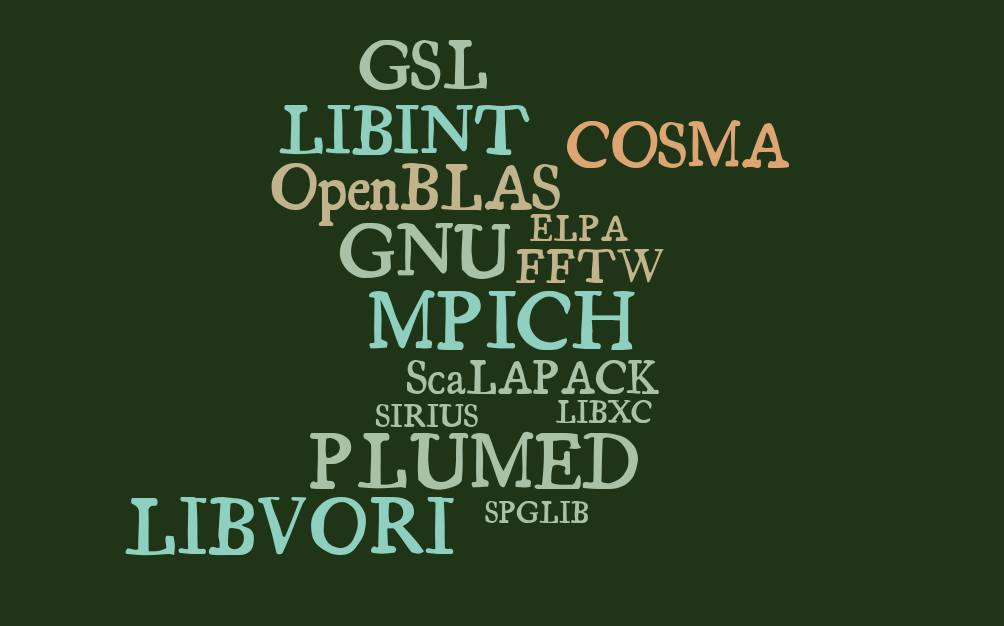
\includegraphics[width=0.7\linewidth]{fig/cp2k-lib.jpg}
  \caption{ไลบรารี่ที่โปรแกรม CP2K ใช้ในการช่วยคำนวณ}
  \label{fig:cp2k_lib}
\end{figure}

ผมจะอธิบาย Library ที่สำคัญ ๆ บางอันที่ CP2K ใช้ ดังนี้

\begin{description}
  \item[GNU] แน่นอนว่าเราต้องคอมไพล์ Source Code ดังนั้นเราจะต้องใช้ตัวคอมไพล์ (Compiler) ซึ่ง CP2K เลือกใช้ GNU เป็น Compiler

  \item[OpenBLAS กับ ScaLAPACK]  สำหรับ Linear Algebraic Calculation เช่น Matrix-vector, Matrix-matrix Multiplication

  \item[MPICH] อยากจะรันโปรแกรมแบบขนานโดยใช้ MPI ก็ต้องหา Implementation ที่จะมารันโค้ดของเรา ซึ่ง MPICH ก็เป็นหนึ่งใน
    Implementation ของ MPI ที่ CP2K เลือกใช้

  \item[FFTW] สำหรับทำฟูเรียร์ทรานฟอร์มในการคำนวณ DFT หรือแปลงจาก Real Space ไปเป็น Reciprocal Space สำหรับการคำนวณ
    Electrostatics โดยใช้ Plane Wave Electron Density

  \item[LIBXC] เป็น Library ที่ให้เราสามารถนำ DFT Functional มาใช้ได้เลยโดยไม่ต้อง Implement เอง
\end{description}

สรุปก็คือจะเห็นได้ว่าการเขียนโค้ดของโปรแกรมเคมีควอนตัมนั้นมีความซับซ้อนมากดังนั้นเรามีสองทางเลือกคือ

\begin{enumerate}[topsep=0pt,noitemsep]
  \setlength\itemsep{1em}
  \item ใช้ Library ที่มีอยู่แล้วสำหรับการทำงานเฉพาะจุด

  \item เขียนโค้ดทั้งหมดเองเลย
\end{enumerate}

แน่นอนว่าถ้าเราเลือกวิธีแรกก็จะประหยัดเวลาไปได้เยอะมากและเวลาที่เราคอมไพล์โปรแกรมก็ขอแค่ Link กับ Library ต่าง ๆ ก็รันโปรแกรมได้แล้ว%
และทำให้ขนาดของตัวโปรแกรมของเรา (ขนาดของ Binary Files) นั้นมีขนาดไม่ใหญ่มากเกินไปด้วย (เช่นหลักสิบ-ร้อยเมกะไบต์)

อย่างไรก็ตามโปรแกรมสำหรับจำลองระบบโมเลกุลหลาย ๆ โปรแกรมก็ไม่ได้ใช้ Library เหล่านี้และเลือกใช้วิธีที่ 2 ก็คือการเขียนโค้ดสำหรับการ%
คำนวณส่วนต่าง ๆ เองเลยเนื่องด้วยเหตุหลายข้อ เช่น การเขียนโค้ดทั้งหมดภายใน Framework โปรแกรมเดียวกันนั้นจะทำให้โค้ดมีประสิทธิภาพและ%
ทำงานร่วมกันได้ดี (Compatibility), ง่ายต่อการดูแลรักษาและปรับปรุงโค้ดเพราะว่า Developers นั้นรู้และเข้าใจการทำงานของโค้ดทั้งหมด,
ถึงแม้ว่าโปรแกรมที่เขียนโค้ดทั้งหมดเองเมื่อถูกคอมไพล์แล้วจะได้ออกมาเป็น Binary File ที่มีขนาดนั้นใหญ่มาก ๆ เช่น หลายกิกะไบต์ แต่ว่าก็มี%
ความคล่องตัวในการใช้งานเพราะว่าไม่ต้องติดตั้ง Library อื่น ๆ เพิ่มเติม

นอกจากนี้แล้วการที่ใช้ Library หลาย ๆ ตัวแบบนี้ก็มีจุดอ่อนบางข้อที่เราควรจะต้องรู้ไว้นั่นก็คือการเข้ากันได้ (Compatibility) ระหว่าง Library
หรือเวอร์ชันซึ่งก็อาจจะทำให้เราปวดหัวได้ถ้าหากว่า Library บางตัวมีการอัพเดทเวอร์ชันใหม่แล้ว Conflict กับ Library ตัวอื่น

%----------------------------------------
\section{ทักษะและเครื่องมือสำหรับการเขียนโปรแกรมคำนวณทางวิทยาศาสตร์}
%----------------------------------------

\noindent \textbf{ภาษาคอมพิวเตอร์}

\begin{itemize}[topsep=0pt]
  \item ภาษาสคริปต์ (Scripting Language): Bash, Python

  \item ภาษาระดับล่างที่เป็น Object-Oriented Programming: C++, Fortran

  \item ภาษาเชิงสัญลักษณ์ (Symbolic Programming): Mathematica, SymPy
\end{itemize}

\noindent \textbf{โปรแกรมสำหรับการเขียนโค้ด}

\begin{itemize}[topsep=0pt]
  \item Vi/Vim, Nano

  \item VS Code, Atom, Eclipse, Sublime, Notepad++
\end{itemize}

\noindent \textbf{พื้นฐานการเขียนโปรแกรม}

\begin{itemize}[topsep=0pt]
  \item ชนิดของตัวแปร (Variable Types)

  \item ตัวดำเนินการหรือโอเปอร์เรเตอร์ (Operator)

  \item Control Statements เช่น For, Do, If-Else, Case

  \item ฟังก์ชัน (Function)

  \item Vairable Scope และ Reference Types

  \item คลาส (Class) และวัตถุ (Objects)
\end{itemize}

\noindent \textbf{ภาษาคอมพิวเตอร์ระดับล่าง}

\noindent \underline{ภาษา C}

\begin{itemize}[topsep=0pt]
  \item Function, Pointer, Storage Class

  \item Enum, Struct, Union

  \item Preprocessor

  \item Operator, Memory Management, Array

  \item การจัดการไฟล์ (File Handling)
\end{itemize}

\noindent \textbf{ภาษาคอมพิวเตอร์ระดับสูง}

\noindent \underline{ภาษา Python}

\begin{itemize}[topsep=0pt]
  \item Pip และ Conda: ตัวช่วยจัดการไลบรารี่ของ Python

  \item NumPy: จัดการและคำนวณ Array (เวกเตอร์, เมทริกซ์)

  \item Numba: JIT Compiler สำหรับ NumPy

  \item Jax: ทำ Autograd (Gradient Comptuation) สำหรับ NumPy Array

  \item SciPy: ไลบรารี่ที่รวมรวบฟังก์ชันทางคณิตศาสตร์และวิทยาศาสตร์

  \item Scikit-learn: ไลบรารี่สำหรับทำสถิติ, Optimization, และ Curve Fitting รวมถึง Machine Learning

  \item Matplotlib, Plotly: พลอตกราฟ

  \item Theano: คำนวณเชิงตัวเลข (Numerical Computation)

  \item SCOOP: โมดูลสำหรับการทำโปรแกรมแบบขนาน (Parallel Programming)

  \item NetworkX: ไลบรารี่สำหรับ Graph
\end{itemize}

\noindent \underline{ภาษา C++}

\begin{itemize}[topsep=0pt]
  \item Type of variable: signed, unsigned, long, double, etc.

  \item Loops, conditional Statement

  \item Standard libraries: vector, rand

  \item Understanding header (`.hpp`) and source file (\texttt{.cpp} or \texttt{.cc})

  \item Preprocessor (\texttt{\#if}, \texttt{\#ifdef}, \texttt{\#ifndef}, \texttt{\#define}, etc.)

  \item Function, class, struct, template

  \item Declaration

  \item namespace, const, attribute, pointer, pass by reference, static_assert

  \item Initialization

  \item casting, lambda expression, encapsulation, file handling, exception handling
\end{itemize}

\noindent \underline{ภาษา Fortran}

\begin{itemize}[topsep=0pt]
  \item เรียนรู้ภาษา Fortran ที่เป็น Modern Fortran ตั้งแต่เวอร์ชัน 2003 เป็นต้นไป

  \item โมดูล (Module), โปรแกรมย่อยหรือซับรูทีน (Subroutine), ฟังก์ชัน (Function)

  \item Array ทั้งแบบที่ปรับเปลี่ยนได้ (Allocatable) และแบบหลายมิติ (Multidimentional)

  \item Operator Overloading, Flow control

  \item Derived Type

  \item Callback

  \item การเขียนโปรแกรมเชื่อมโยงกับภาษาอื่น เช่น Python หรือ C++

  \item การใช้ GNU Library ในการคอมไพล์

  \item การจัดการหน่วยความจำ (Memory Allocation): Stack, Heap, Global Memory
\end{itemize}

\noindent \underline{ไลบรารี่สำหรับการคำนวณทางคณิตศาสตร์}

\begin{itemize}[topsep=0pt]
  \item BLAS (OpenBLAS)

  \item LAPACK: สำหรับคำนวณ Linear Algebra

  \item ScaLAPACK: เป็น LAPACK สำหรับซุปเปอร์คอมพิวเตอร์

  \item Intel MKL (Intel oneAPI)

  \item FFTW: สำหรับคำนวณ Discrete Fourier Transform ในหนึ่งมิติหรือมากกว่าหนึ่งมิติก็ได้

  \item Eigen: สำหรับคำนวณ Linear Algebra

  \item Boost: ไลบรารี่ที่รวบรวมฟังก์ชันต่าง ๆ สำหรับช่วยเขียนโปรแกรมภาษา C++ เช่น regex, serialization
\end{itemize}

\noindent \underline{เครื่องมือช่วยการพัฒนาซอฟต์แวร์}

\begin{itemize}[topsep=0pt]
  \item การทำ Code Optimization

  \item การทำ Benchmarking และ Scaling

  \item ความซับซ้อนเชิงการคำนวณ (Computational Complexity)

  \item Static และ Dynamic Libraries

  \item คอมไพเลอร์ Compiling (g++, gcc) และ Linking (ld)

  \item เครื่องมือสำหรับช่วยการคอมไพล์โค้ด: autoconf, configure, make, cmake, automake

  \item เครื่องมือสำหรับช่วยการ Debug: gdb สำหรับการ Debug ทั่วไปและ Valgrind สำหรับการวิเคราะห์ Memory Leak

  \item การทำ Source Code Control: Git (GitHub และ GitLab)

  \item การทำ Documentation: Sphinx (สำหรับ markdown และ reStructuredText), Doxygen
\end{itemize}

\noindent \underline{ไลบรารี่สำหรับเคมีควอนตัม}

\begin{itemize}[topsep=0pt]
  \item libxc: ไลบรารี่ที่รวบรวม XC Function สำหรับ DFT ซึ่งเราสามารถนำมาใช้งานได้เลย

  \item libint: ไลบรารี่ที่ช่วยในการคำนวณ Gaussian Integrals

  \item libcint: ไลบรารี่ที่ช่วยในการคำนวณ GTO Integrals
\end{itemize}

%----------------------------------------
\section{เขียนโปรแกรมวิเคราะห์ Molecular Geometry (ภาษา C++)}
%----------------------------------------

โปรแกรมแรกที่ผู้อ่านจะได้ศึกษาและฝึกเขียนตามก็คือโปรแกรมสำหรับวิเคราะห์เรขาคณิตเชิงโครงสร้าง Structural Geometry ของโมเลกุล
โดยเราจะใช้ภาษา C++ กันครับ ซึ่งภาษา C++ นั้นเป็นภาษาที่มีประสิทธิภาพสูงมากและถูกใช้อย่างแพร่หลายในการทำงานวิจัยเคมีควอนตัม
(รวมถึงสาขาอื่น ๆ ด้วย) และโปรแกรมสำหรับการวิเคราะห์อันนี้ไม่มีความซับซ้อนมาก

\noindent \bful{Step 1: อ่านไฟล์ Coordinates}

\vspace{5pt}

\begin{lstlisting}[style=MyC++]
#include <iostream>
#include <fstream>
#include <iomanip>
#include <cstdio>

using namespace std;

int main() 
{
  ifstream input("geom.dat");

  int natom;
  input >> natom;

  int *zval = new int[natom];
  double *x = new double[natom];
  double *y = new double[natom];
  double *z = new double[natom];

  for(int i=0; i < natom; i++)
    input >> zval[i] >> x[i] >> y[i] >> z[i];
  
  input.close();

  cout << "Number of atoms: " << natom << endl;
  cout << "Input Cartesian coordinates:\n";
  for(int i=0; i < natom; i++)
    printf("%d %20.12f %20.12f %20.12f\n", (int) zval[i], x[i], y[i], z[i]);

  delete[] zval;
  delete[] x;  delete[] y;  delete[] z;

  return 0;
}
\end{lstlisting}

\vspace{5pt}

จากตัวอย่างโค้ดด้านบนนั้นเริ่มการทำงานด้วยการอ่านไฟล์ Coordinates ของอะตอมในโมเลกุลซึ่งมีหน่วยคือ bohr โดยผู้อ่านอาจจะลองใช้ตัวอย่าง%
โมเลกุลเล็ก ๆ เช่น Acetaldehyde ซึ่งมี Coordinates ดังนี้

\begin{Verbatim}[frame=single]
  7
  6  0.000000000000     0.000000000000     0.000000000000
  6  0.000000000000     0.000000000000     2.845112131228
  8  1.899115961744     0.000000000000     4.139062527233
  1 -1.894048308506     0.000000000000     3.747688672216
  1  1.942500819960     0.000000000000    -0.701145981971
  1 -1.007295466862    -1.669971842687    -0.705916966833
  1 -1.007295466862     1.669971842687    -0.705916966833
\end{Verbatim}

\noindent โดยที่เลข 7 ในบรรทัดแรกนั้นคือจำนวนอะตอมและบรรทัดที่เหลือนั้นคือพิกัดตำแหน่ง x, y, z ของอะตอมแต่ละตัว เมื่อโปรแกรมเปิดไฟล์%
แล้วสิ่งที่จะทำถัดไปก็คือการอ่านข้อมูลแต่ละบรรทัดและเก็บข้อมูลไว้ จริง ๆ แล้วเราสามารถ Simplify โค้ดตัวอย่างอันนี้ให้มีความเป็นระเบียบมากขึ้น%
โดยการใช้ Class เช่น เราสามารถสร้างไฟล์ header ที่ชื่อ \inlinehighlight{molecule.h} แล้วทำการเรียกใช้งาน Class ในไฟล์โปรแกรม
\inlinehighlight{molecule.cpp} ได้ดังนี้

\vspace{5pt}

\begin{lstlisting}[style=MyC++]
#include "molecule.h"
#include <iostream>
#include <fstream>
#include <iomanip>
#include <cstdio>

using namespace std;

int main()
{
  Molecule mol("geom.dat", 0);

  cout << "Number of atoms: " << mol.natom << endl;
  cout << "Input Cartesian coordinates:\n";
  mol.print_geom();

  return 0;
}
\end{lstlisting}

\vspace{5pt}

\noindent ทีนี้สิ่งที่ผมอยากให้ผู้อ่านทำก็คือลองฝึกเขียนโค้ดของไฟล์ \inlinehighlight{molecule.h} โดยดัดแปลงจากโค้ดด้านบนครับ

\noindent \bful{Step 2: คำนวณความยาวพันธะ (Bond Lengths)}

คำนวณระยะห่างระหว่างอะตอม (Interatomic Distances) โดยใช้สมการดังต่อไปนี้

\begin{equation}
  R_{ij}
  =
  \sqrt{
    (x_{i} - x_{j})^{2}
    + (y_{i} - y_{j})^{2}
    + (z_{i} - z_{j})^{2}
  }
\end{equation}

\noindent โดยที่ $x, y, z$ คือ Cartesian Coordinates และ $i$ กับ $j$ คือเลข Index ของอะตอม

สำหรับการเขียนโปรแกรมเพื่อคำนวณ Distance นั้นเราจะต้องคำนึงถึงการจัดการหน่วยความจำ (Memory Allocation) ด้วยเพื่อให้โปรแกรมของเรา%
นั้นมีประสิทธิภาพมากที่สุดซึ่งนั่นก็จะเกี่ยวข้องกับการเลือกวิธีในการเก็บข้อมูลของระยะห่างระหว่างอะตอม ในการหาความยาวระหว่างอะตอมของทุก ๆ
คู่นั้นสามารถใช้เมทริกซ์มาเก็บข้อมูลได้ซึ่งขนาดของเมทริกซ์จะเป็น $N \times N$ โดยที่ $N$ คือจำนวนอะตอม ในการใช้เมทริกซ์นั้นเราจำเป็นที่%
จะต้องจัดสรร (Allocate) หน่วยความจำซึ่งทำได้สองวิธีคือ

\noindent $\bullet$ 1. ใช้ Static Two-Dimensional Array

\vspace{5pt}

\begin{lstlisting}[style=MyC++]
double R[50][50];
\end{lstlisting}

\vspace{5pt}

\noindent $\bullet$ 2. ใช้ Dynamic Allocation โดยการใช้คลาส \inlinehighlight{Molecule}

\vspace{5pt}

\begin{lstlisting}[style=MyC++]
double **R = new double* [mol.natom];
for(int i=0; i < mol.natom; i++)
  R[i] = new double[mol.natom];
\end{lstlisting}

\vspace{5pt}

\noindent แล้วก็อย่าลืมลบหน่วยความจำหลังจากที่คำนวณเสร็จแล้วด้วย ดังนี้

\vspace{5pt}

\begin{lstlisting}[style=MyC++]
for(int i=0; i < mol.natom; i++)
  delete[] R[i];
delete[] R;
\end{lstlisting}

\vspace{5pt}

ขั้นตอนต่อไปก็คือการสร้างเมทริกซ์ขึ้นมาซึ่งสามารถทำได้โดยใช้ For Loop ในการวนไปเรื่อย ๆ ตามเลข Index ของอะตอม

\vspace{5pt}

\noindent แล้วก็อย่าลืมลบหน่วยความจำหลังจากที่คำนวณเสร็จแล้วด้วย ดังนี้

\vspace{5pt}

\begin{lstlisting}[style=MyC++]
...
#include <cmath>
...

for(int i=0; i < mol.natom; i++) {
  for(int j=0; j < mol.natom; j++) {
      R[i][j] = 
        sqrt(
          (mol.geom[i][0]-mol.geom[j][0])*(mol.geom[i][0]-mol.geom[j][0])
        + (mol.geom[i][1]-mol.geom[j][1])*(mol.geom[i][1]-mol.geom[j][1])
        + (mol.geom[i][2]-mol.geom[j][2])*(mol.geom[i][2]-mol.geom[j][2]) 
        );
  }
}
\end{lstlisting}

\vspace{5pt}

ลำดับต่อไปคือการแสดงค่าความยาวที่คำนวณได้โดยเราก็จะใช้ For Loop เหมือนเดิม

\vspace{5pt}

\begin{lstlisting}[style=MyC++]
for(int i=0; i < mol.natom; i++)
  for(int j=0; j < i; j++)
    printf("%d %d %8.5f\n", i, j, R[i][j]);
\end{lstlisting}

\vspace{5pt}

ขั้นตอนสุดท้ายคือการทำให้โค้ดนั้นมีความเรียบร้อยและมีประสิทธิภาพมากขึ้น โดยเราสามารถนำโค้ดด้านบนที่เราได้เขียนไว้สร้างเป็นฟังก์ชันใหม่ที่ชื่อว่า
\ih{bond()} ในคลาส \ih{Molecule} ได้ดังนี้

\vspace{5pt}

\begin{lstlisting}[style=MyC++]
double Molecule::bond(int a, int b)
{
  return sqrt( (geom[a][0]-geom[b][0])*(geom[a][0]-geom[b][0])
              + (geom[a][1]-geom[b][1])*(geom[a][1]-geom[b][1])
              + (geom[a][2]-geom[b][2])*(geom[a][2]-geom[b][2]) );
}
\end{lstlisting}

\vspace{5pt}

แล้วก็โปรแกรมของเราก็จะมีหน้าตาเป็นแบบนี้

\vspace{5pt}

\begin{lstlisting}[style=MyC++]
#include "molecule.h"
#include <iostream>
#include <fstream>
#include <iomanip>
#include <cstdio>
#include <cmath>

using namespace std;
  
int main()
{
  Molecule mol("geom.dat", 0);
  
  cout << "Number of atoms: " << mol.natom << endl;
  cout << "Input Cartesian coordinates:\n";
  mol.print_geom();
  
  cout << "\nInteratomic distances (bohr):\n";
  for(int i=0; i < mol.natom; i++)
    for(int j=0; j < i; j++)
      printf("%d %d %8.5f\n", i, j, mol.bond(i,j));
      
  return 0;
}
\end{lstlisting}

\vspace{5pt}

\noindent ซึ่งก็จะมีเอาต์พุตดังต่อไปนี้

\vspace{5pt}

\begin{lstlisting}[style=MyC++]
Number of atoms: 7
Input Cartesian coordinates:
6     0.000000000000     0.000000000000     0.000000000000
6     0.000000000000     0.000000000000     2.845112131228
8     1.899115961744     0.000000000000     4.139062527233
1    -1.894048308506     0.000000000000     3.747688672216
1     1.942500819960     0.000000000000    -0.701145981971
1    -1.007295466862    -1.669971842687    -0.705916966833
1    -1.007295466862     1.669971842687    -0.705916966833

Interatomic distances (bohr):
1 0  2.84511
2 0  4.55395
2 1  2.29803
3 0  4.19912
3 1  2.09811
3 2  3.81330
4 0  2.06517
4 1  4.04342
4 2  4.84040
4 3  5.87463
5 0  2.07407
5 1  4.05133
5 2  5.89151
5 3  4.83836
5 4  3.38971
6 0  2.07407
6 1  4.05133
6 2  5.89151
6 3  4.83836
6 4  3.38971
6 5  3.33994
\end{lstlisting}

\vspace{5pt}

\noindent โดยที่ \ih{bond()} คือ Member Function ของ \ih{Molecule} ซึ่งเราสามารถเรียกใช้ข้อมูลของ Geometry (Coordinates)
ได้ผ่าน \ih{geom} โดยไม่จำเป็นต้องเรียกใช้ผ่าน \ih{mol.geom}

\noindent \bful{Step 3: คำนวณมุมพันธะ (Bond Angles)}

เราสามารถคำนวณมุมพันธะทุกมุมที่เป็นไปได้ทั้งหมดของโมเลกุล (ระหว่างอะตอม $i, j, k$) $\phi_{ijk}$ ได้ด้วยสมการดังต่อไปนี้

\begin{equation}
  \label{eq:cos_bond_angle}
  \cos \phi_{ijk} = \tilde{e}_{ji} \cdot \tilde{e}_{jk}
\end{equation}

\noindent โดยที่ $e_{ij}$ คือเวกเตอร์หนึ่งหน่วย (Unit Vector) ระหว่างอะตอมซึ่งสามารถคำนวณได้ด้วยสมการดังต่อไปนี้

\begin{align*}
  e^{x}_{ij}
  = \frac{
    -(x_{i} - x_{j})
  }
  {
    R_{ij}
  } \\
  e^{y}_{ij}
  = \frac{
    -(y_{i} - y_{j})
  }
  {
    R_{ij}
  } \\
  e^{z}_{ij}
  = \frac{
    -(z_{i} - z_{j})
  }
  {
    R_{ij}
  }
\end{align*}

\vspace{5pt}

โดยเราจะสร้างฟังก์ชันสำหรับคำนวณมุมพันธะซึ่งก็คือ Inverse ของฟังก์ชัน Cosine ของสมการที่ \eqref{eq:cos_bond_angle} แล้วเพิ่มฟังก์ชัน%
นี้เข้าไปในไฟล์ \ih{molecule.cpp} ดังนี้

\vspace{5pt}

\begin{lstlisting}[style=MyC++]
// Returns the value of the unit vector between atoms a and b
// in the cart direction (cart=0=x, cart=1=y, cart=2=z)
double Molecule::unit(int cart, int a, int b)
{
  return -(geom[a][cart]-geom[b][cart])/bond(a,b);
}

// Returns the angle between atoms a, b, and c in radians
double Molecule::angle(int a, int b, int c)
{
  return acos(unit(0,b,a) * unit(0,b,c) + unit(1,b,a) * unit(1,b,c) + unit(2,b,a) * unit(2,b,c));
}
\end{lstlisting}

\vspace{5pt}

\noindent นอกจากนี้เราจะต้องเพิ่ม Declaration ของ Member Function เข้าไปในไฟล์ \ih{molecule.h} ด้วย ดังนี้

\vspace{5pt}

\begin{lstlisting}[style=MyC++]
#include <string>

using namespace std;

class Molecule
{
  public:
    int natom;
    int charge;
    int *zvals;
    double **geom;
    string point_group;

    void print_geom();
    void rotate(double phi);
    void translate(double x, double y, double z);
    double bond(int atom1, int atom2);
    double angle(int atom1, int atom2, int atom3);
    double torsion(int atom1, int atom2, int atom3, int atom4);
    double unit(int cart, int atom1, int atom2);

    Molecule(const char *filename, int q);
    ~Molecule();
};
\end{lstlisting}

\vspace{5pt}

แล้วโปรแกรมสำหรับคำนวณมุมพันธะที่สมบูรณ์นั้นจะมีหน้าตาแบบนี้

\vspace{5pt}

\begin{lstlisting}[style=MyC++]
#include "molecule.h"
#include <iostream>
#include <fstream>
#include <iomanip>
#include <cstdio>
#include <cmath>

using namespace std;
  
int main()
{
  Molecule mol("geom.dat", 0);
  
  cout << "Number of atoms: " << mol.natom << endl;
  cout << "Input Cartesian coordinates:\n";
  mol.print_geom();

  cout << "\nBond angles:\n";
  for(int i=0; i < mol.natom; i++) {
    for(int j=0; j < i; j++) {
      for(int k=0; k < j; k++) {
        if(mol.bond(i,j) < 4.0 && mol.bond(j,k) < 4.0)
          printf("%2d-%2d-%2d %10.6f\n", i, j, k, mol.angle(i,j,k)*(180.0/acos(-1.0)));
      }
    }
  }

  return 0;
}
\end{lstlisting}

\vspace{5pt}

\noindent โดยที่เราใช้ \cppinline{acos(-1.0)} ในการประมาณค่า $\pi$

เมื่อเรารันโปรแกรมด้านบนจะได้เอาต์พุตแบบนี้

\vspace{5pt}

\begin{lstlisting}
Number of atoms: 7
Input Cartesian coordinates:
6     0.000000000000     0.000000000000     0.000000000000
6     0.000000000000     0.000000000000     2.845112131228
8     1.899115961744     0.000000000000     4.139062527233
1    -1.894048308506     0.000000000000     3.747688672216
1     1.942500819960     0.000000000000    -0.701145981971
1    -1.007295466862    -1.669971842687    -0.705916966833
1    -1.007295466862     1.669971842687    -0.705916966833

Bond angles:
  2- 1- 0 124.268308
  3- 1- 0 115.479341
  3- 2- 1  28.377448
  5- 4- 0  35.109529
  6- 4- 0  35.109529
  6- 5- 0  36.373677
  6- 5- 4  60.484476
\end{lstlisting}

\vspace{5pt}

\noindent \bful{Step 4: คำนวณมุมบิด (Torsion หรือ Dihedral Angles)}

พารามิเตอร์ลำดับต่อมาที่เราจะคำนวณก็คือมุมบิด (Torsion Angle) สำหรับมุมบิดของอะตอม 4 อะตอมใด ๆ ในโมเลกุล $i, j, k, l$ นั้นมี%
สมการในการคำนวณคือ

\begin{equation}
  \cos \tau_{ijkl}
  =
  \frac{
    (\tilde{e}_{ij} \times \tilde{e}_{jk})
    \cdot
    (\tilde{e}_{jk} \times \tilde{e}_{kl})
  }
  {
    \sin \theta_{ijk}
    \sin \theta_{jkl}
  }
\end{equation}

\noindent สิ่งที่ต้องระวังในการคำนวณ Torsion Angle ก็คือเครื่องหมายของมุมซึ่งจะเป็นบวกหรือลบนั้นก็คือขึ้นอยู่กับว่าเวกเตอร์นั้นมีทิศทางไปทาง%
ไหนเมื่อเทียบกับระนาบ

\begin{itemize}[topsep=0pt,noitemsep]
  \setlength\itemsep{1em}
  \item มุมบิดของอะตอม $i-j-k-l$ เป็นบวกเมื่อเวกเตอร์ตามแนวอะตอม $k-l$ นั้นวางตัวไปทางด้านขวาของระนาบที่สร้างจากอะตอม $i-j-k$
        เมื่อมองจากทิศทางของเวกเตอร์ $j-k$

  \item มุมบิดของอะตอม $i-j-k-l$ เป็นลบเมื่อเวกเตอร์ตามแนวอะตอม $k-l$ นั้นวางตัวไปทางด้านซ้ายของระนาบที่สร้างจากอะตอม $i-j-k$
        เมื่อมองจากทิศทางของเวกเตอร์ $j-k$
\end{itemize}

\vspace{5pt}

โปรแกรมสำหรับคำนวณ Torsion Angle นั้นมีดังนี้ เริ่มต้นด้วยการสร้าง Member Function ของคลาส \ih{Molecule}

\vspace{5pt}

\begin{lstlisting}[style=MyC++]
// Computes the angle between planes a-b-c and b-c-d
double Molecule::torsion(int a, int b, int c, int d)
{
  double eabc_x = (unit(1,b,a)*unit(2,b,c) - unit(2,b,a)*unit(1,b,c));
  double eabc_y = (unit(2,b,a)*unit(0,b,c) - unit(0,b,a)*unit(2,b,c));
  double eabc_z = (unit(0,b,a)*unit(1,b,c) - unit(1,b,a)*unit(0,b,c));

  double ebcd_x = (unit(1,c,b)*unit(2,c,d) - unit(2,c,b)*unit(1,c,d));
  double ebcd_y = (unit(2,c,b)*unit(0,c,d) - unit(0,c,b)*unit(2,c,d));
  double ebcd_z = (unit(0,c,b)*unit(1,c,d) - unit(1,c,b)*unit(0,c,d));

  double exx = eabc_x * ebcd_x;
  double eyy = eabc_y * ebcd_y;
  double ezz = eabc_z * ebcd_z;

  double tau = (exx + eyy + ezz)/(sin(angle(a,b,c)) * sin(angle(b,c,d)));

  if(tau < -1.0) tau = acos(-1.0);
  else if(tau > 1.0) tau = acos(1.0);
  else tau = acos(tau);

  // Compute the sign of the torsion 
  double cross_x = eabc_y * ebcd_z - eabc_z * ebcd_y;
  double cross_y = eabc_z * ebcd_x - eabc_x * ebcd_z;
  double cross_z = eabc_x * ebcd_y - eabc_y * ebcd_x;
  double norm = cross_x*cross_x + cross_y*cross_y + cross_z*cross_z;
  cross_x /= norm;
  cross_y /= norm;
  cross_z /= norm;
  double sign = 1.0;
  double dot = cross_x*unit(0,b,c)+cross_y*unit(1,b,c)+cross_z*unit(2,b,c);
  if(dot < 0.0) sign = -1.0;

  return tau*sign;
}
\end{lstlisting}

\vspace{5pt}

แล้วเราก็เรียกใช้ฟังก์ชันใหม่ที่เราเพิ่งสร้างไว้ในโปรแกรมหลักของเราได้ดังนี้

\vspace{5pt}

\begin{lstlisting}[style=MyC++]
#include <iostream>
#include <fstream>
#include <iomanip>
#include <cstdio>
#include <cmath>
#include "molecule.h"

using namespace std;

int main()
{
  Molecule mol("geom.dat", 0);

  cout << "Number of atoms: " << mol.natom << endl;
  cout << "Input Cartesian coordinates:\n";
  mol.print_geom();

  cout << "\nTorsional angles:\n";
  for(int i=0; i < mol.natom; i++) {
    for(int j=0; j < i; j++) {
      for(int k=0; k < j; k++) {
        for(int l=0; l < k; l++) {
          if(mol.bond(i,j) < 4.0 && mol.bond(j,k) < 4.0 && mol.bond(k,l) < 4.0)
            printf("%2d-%2d-%2d-%2d %10.6f\n", i, j, k, l, mol.torsion(i,j,k,l)*(180.0/acos(-1.0)));
        }
      }
    }
  }

  return 0;
}
\end{lstlisting}

\vspace{5pt}

\noindent เมื่อเรารันโปรแกรมด้านบนเราจะได้เอาต์พุตดังนี้

\vspace{5pt}

\begin{lstlisting}[style=MyC++]
Number of atoms: 7
Input Cartesian coordinates:
6       0.000000000000       0.000000000000       0.000000000000
6       0.000000000000       0.000000000000       2.845112131228
8       1.899115961744       0.000000000000       4.139062527233
1      -1.894048308506       0.000000000000       3.747688672216
1       1.942500819960       0.000000000000      -0.701145981971
1      -1.007295466862      -1.669971842687      -0.705916966833
1      -1.007295466862       1.669971842687      -0.705916966833

Torsional angles:
  3- 2- 1- 0 180.000000
  6- 5- 4- 0  36.366799  
\end{lstlisting}

\vspace{5pt}

\noindent \bful{Step 5: คำนวณจุดศูนย์กลางมวล มุมบิด (Center of Mass)}

\noindent \underline{แบบฝึกหัด}: ให้ลองเขียนโปรแกรมคำนวณจุดศูนย์กลางมวลของโมเลกุล โดยสมการที่ใช้ในการคำนวณนั้นสามารถดูได้จาก
Wikipedia ครับ

\noindent \underline{เฉลย}

\vspace{5pt}

\begin{lstlisting}[style=MyC++]
#include "molecule.h"
#include "masses.h"

#include <iostream>
#include <fstream>
#include <iomanip>
#include <cstdio>
#include <cmath>

using namespace std;

int main()
{
  Molecule mol("geom.dat", 0);

  cout << "Number of atoms: " << mol.natom << endl;
  cout << "Input Cartesian coordinates:\n";
  mol.print_geom();

  cout << "Interatomic distances (bohr):\n";
  for(int i=0; i < mol.natom; i++)
    for(int j=0; j < i; j++)
      printf("%d %d %8.5f\n", i, j, mol.bond(i,j));

  cout << "\nBond angles:\n";
  for(int i=0; i < mol.natom; i++) {
    for(int j=0; j < i; j++) {
      for(int k=0; k < j; k++) {
        if(mol.bond(i,j) < 4.0 && mol.bond(j,k) < 4.0)
          printf("%2d-%2d-%2d %10.6f\n", i, j, k, mol.angle(i,j,k)*(180.0/acos(-1.0)));
      }
    }
  }

  cout << "\nOut-of-Plane angles:\n";
  for(int i=0; i < mol.natom; i++) {
    for(int k=0; k < mol.natom; k++) {
      for(int j=0; j < mol.natom; j++) {
        for(int l=0; l < j; l++) {
          if(i!=j && i!=k && i!=l && j!=k && k!=l && mol.bond(i,k) < 4.0 && 
              mol.bond(k,j) < 4.0 && mol.bond(k,l) < 4.0)
              printf("%2d-%2d-%2d-%2d %10.6f\n", i, j, k, l, mol.oop(i,j,k,l)*(180.0/acos(-1.0)));
        }
      }
    }
  }

  cout << "\nTorsional angles:\n\n";
  for(int i=0; i < mol.natom; i++) {
    for(int j=0; j < i; j++) {
      for(int k=0; k < j; k++) {
        for(int l=0; l < k; l++) {
          if(mol.bond(i,j) < 4.0 && mol.bond(j,k) < 4.0 && mol.bond(k,l) < 4.0)
            printf("%2d-%2d-%2d-%2d %10.6f\n", i, j, k, l, mol.torsion(i,j,k,l)*(180.0/acos(-1.0)));
        }
      }
    }
  }
  
  /* find the center of mass (COM) */
  double M = 0.0;
  for(int i=0; i < mol.atom; i++) M += an2masses[(int) mol.zvals[i]];

  double xcm=0.0;
  double ycm=0.0;
  double zcm=0.0;
  double mi;
  for(int i=0; i < mol.atom; i++) {
    mi = an2masses[(int) mol.zvals[i]];
    xcm += mi * mol.geom[i][0];
    ycm += mi * mol.geom[i][1];
    zcm += mi * mol.geom[i][2];
  }
  xcm /= M;
  ycm /= M;
  zcm /= M;
  printf("\nMolecular center of mass: %12.8f %12.8f %12.8f\n", xcm, ycm, zcm);

  mol.translate(-xcm, -ycm, -zcm);

  return 0;
}
\end{lstlisting}

\vspace{5pt}

\noindent เมื่อเรารันโปรแกรมด้านบนเราจะได้เอาต์พุตดังนี้

\vspace{5pt}

\begin{lstlisting}[style=MyC++]
Number of atoms: 7
Input Cartesian coordinates:
6       0.000000000000       0.000000000000       0.000000000000
6       0.000000000000       0.000000000000       2.845112131228
8       1.899115961744       0.000000000000       4.139062527233
1      -1.894048308506       0.000000000000       3.747688672216
1       1.942500819960       0.000000000000      -0.701145981971
1      -1.007295466862      -1.669971842687      -0.705916966833
1      -1.007295466862       1.669971842687      -0.705916966833
Interatomic distances (bohr):
1 0  2.84511
2 0  4.55395
2 1  2.29803
3 0  4.19912
3 1  2.09811
3 2  3.81330
4 0  2.06517
4 1  4.04342
4 2  4.84040
4 3  5.87463
5 0  2.07407
5 1  4.05133
5 2  5.89151
5 3  4.83836
5 4  3.38971
6 0  2.07407
6 1  4.05133
6 2  5.89151
6 3  4.83836
6 4  3.38971
6 5  3.33994

Bond angles:
  0- 1- 2 124.268308
  0- 1- 3 115.479341
  0- 4- 5  35.109529
  0- 4- 6  35.109529
  0- 5- 6  36.373677
  1- 2- 3  28.377448
  4- 5- 6  60.484476

Out-of-plane angles:
  0- 3- 1- 2  -0.000000
  0- 6- 4- 5  19.939726
  0- 6- 5- 4 -19.850523
  0- 5- 6- 4  19.850523
  1- 5- 0- 4  53.678778
  1- 6- 0- 4 -53.678778
  1- 6- 0- 5  54.977064
  2- 3- 1- 0   0.000000
  3- 2- 1- 0  -0.000000
  4- 5- 0- 1 -53.651534
  4- 6- 0- 1  53.651534
  4- 6- 0- 5 -54.869992
  4- 6- 5- 0  29.885677
  4- 5- 6- 0 -29.885677
  5- 4- 0- 1  53.626323
  5- 6- 0- 1 -56.277112
  5- 6- 0- 4  56.194621
  5- 6- 4- 0 -30.558964
  5- 4- 6- 0  31.064344
  6- 4- 0- 1 -53.626323
  6- 5- 0- 1  56.277112
  6- 5- 0- 4 -56.194621
  6- 5- 4- 0  30.558964
  6- 4- 5- 0 -31.064344

Torsional angles:

  3- 2- 1- 0 180.000000
  6- 5- 4- 0  36.366799

Molecular center of mass:   0.64494926   0.00000000   2.31663792
\end{lstlisting}

%----------------------------------------
\section{เขียนโปรแกรม Hartree-Fock SCF (ภาษา Python)}
%----------------------------------------

%----------------------------------------
\subsection{ทำความเข้าใจขั้นตอน SCF กันก่อน}
%----------------------------------------

โปรแกรมเคมีควอนตัมทุกโปรแกรมจะต้องมีส่วนหนึ่งของโปรแกรมที่เป็นโค้ดสำหรับแก้สมการอันหนึ่งซึ่งขาดไม่ได้เลยนั่นก็คือ Roothaan-Hall
Equation โดยใช้วิธี Self-Consistent Field ซึ่งเป็นสมการที่เราใช้ในการคำนวณหาพลังงานของระบบที่เราสนใจ

สมการ Roothaan-Hall นั้นจะเรียกว่าเป็นสมการ HF ที่แปลงร่างมาแล้วก็ได้ สาเหตุที่เราต้องทำการแปลงร่าง HF นั้นก็เพราะว่าเราเขียน
Wavefunction ให้อยู่ในรูปที่มี Basis Function นั่นเอง (Basis Function คือสิ่งที่เราใช้อธิบายออร์บิทัลเชิงอะตอม) โดยเราจะมีสมการ
Roothaan-Hall ทั้งหมด $m$ สมการ โดยที่ $m$ คือจำนวนของ Basis Function (เรามีสมการ HF 1 สมการต่อ 1 MO และการที่เรามี
$m$ Basis Function นั้นก็จะสร้างทั้งหมด $m$ MOs ด้วย), $F$ คือ Fock Matrix ซึ่งก็จะได้จาก Density Matrix แล้ว
Density Matrix ก็คือ Matrix ที่มีสมาชิกเป็นผลคูณระหว่าง Coefficients ของ MO ซึ่งก็จะได้มาจากการประมาณค่าด้วยวิธีเริ่มต้น
(Initial Guess) แบบต่าง ๆ เช่นใช้ H\"{u}ckel Method, ส่วน $S$ นั้นก็คือ Overlap Matrix ซึ่งก็จะเป็น Matrix ที่บอกว่า
Orbitals นั้นสัมพันธ์กันมากน้อยแค่ไหน, และ $\epsilon$ ของแต่ละสมการนั้นก็คือค่าพลังงานของแต่ละ MO นั้นเองซึ่งเป็นสิ่งที่เรา%
ต้องการแก้สมการหามันออกมา ทีนี้เราสามารถยุบรวมสมการ HF สำหรับแต่ละ Basis Function เข้าด้วยกันได้ ซึ่งจะได้ออกมาเป็นตามสมการที่%
สั้นและกระชับขึ้นนั่นก็คือสมการ Roothaan-Hall นั่นเอง ดังนี้ (เขียนในรูปของเมทริกซ์)

\begin{equation}
  \bm{FC} = \bm{SC \varepsilon}
\end{equation}

โดยมี $F$, $C$, และ $S$ แทน Fock Matrix, MO Coefficients Matrix, และ Overlap Matrix ตามลำดับ โดย Matrix
ทั้งสามอันนี้มีขนาดคือ $m \times m$ แล้วก็ $\epsilon$ นั้นก็มีขนาด $m \times m$ ด้วย (มีเฉพาะสมาชิกในแนวทแยงเท่านั้นที่มีค่าไม่เท่ากับ 0)
โดย $C$ มีหน้าตาดังต่อไปนี้

\begin{equation}
  \bm{C}
  =
  \left( \begin{matrix} c_{1,1} & c_{1,2} & ... & c_{1,m} \\
               c_{2,1} & c_{2,2} & ... & c_{2,m} \\
               \vdots  & \vdots  &     & \vdots  \\
               c_{m,1} & c_{m,2} & ... & c_{m,m}
    \end{matrix} \right)
\end{equation}

\noindent และ $\epsilon$

\begin{equation}
  \bm{E}
  =
  \left( \begin{matrix} \epsilon_1 & 0          & ... & 0            \\
               0          & \epsilon_2 & ... & 0            \\
               \vdots     & \vdots     &     & \vdots       \\
               0          & 0          & ... & \epsilon_{m}
    \end{matrix} \right)
\end{equation}

ซึ่งแนวคิดของการแก้ปัญหา SCF นั้นก็คือเราพยายามที่จะหาค่าของ $\bm{C}$ ที่จะทำให้มีพลังงานของระบบนั้นมีค่าน้อยที่สุดเท่าที่จะเป็นไปได้
(Energy Minimization) แต่ว่าเราดันมี $\bm{C}$ อยู่ทั้งสองข้างของสมการ ดังนั้นเราจึงต้องทำการแก้สมการด้านบนโดยการใช้การวนซ้ำ
(Iteration) จนกว่าจะได้ $\bm{C}$ ของทั้งสองข้างของสมการที่เท่ากัน (หรือเกือบจะเท่ากัน) ซึ่งจะทำให้ได้ค่าพลังงาน $\epsilon$ ที่ต่ำที่สุดด้วย

ปัญหาถัดมาก็คือว่าสมการด้านบนนั้นมันเป็น Eigenvalue Problem ในฟอร์มที่ยังแก้ไม่ได้ (แก้ได้แต่ว่าจะได้คำตอบที่ไม่ถูกต้อง) ซึ่งถ้าหากเราสามารถ%
เปลี่ยนจาก $\bm{FC} = \bm{SC \epsilon}$ ให้เป็น $\bm{FC} = \bm{C \epsilon}$ ได้ ก็จะทำให้เราสามารถแก้ Eigenvalue Problem
ได้อย่างมีประสิทธิภาพและได้คำตอบที่ถูกต้อง ดังนั้นเราจึงมีเทคนิคในการแปลงโดยการทำ Orthogonalization ซึ่งถ้าสรุปสั้น ๆ ก็คือว่าเราสามารถ%
แปลงออกมาได้เป็น

\begin{equation}
  \bm{F'C'} = \bm{C'E}
\end{equation}

\noindent โดยที่

\begin{gather}
  \bm{F'} = \bm{S}^{-1/2}\bm{F}\bm{S}^{-1/2} \\
  \bm{C'} = \bm{S}^{-1/2}\boldsymbol{C}
\end{gather}

\noindent ตามวิชา Linear Algebra ถ้าเราต้องการหา Matrix ของ $\epsilon$ เราสามารถใช้วิธี Diagonalization
กับสมการ Roothaan-Hall ได้เพราะว่าสมการนี้มันเป็น Eigenfunction ซึ่งกระบวนการที่จะใช้ในการแก้นั้นก็คือตามขั้นตอนต่อไปนี้

\noindent \textbf{กระบวนการ SCF แบบคร่าว ๆ ตามทฤษฎี}

\begin{enumerate}[topsep=0pt,noitemsep]
  \setlength\itemsep{1em}
  \item เรากำหนดตำแหน่งของอะตอมในโมเลกุล, ประจุ, และทำการเลือก Basis Set

  \item เริ่มคำนวณพลังงานจลน์และพลังงานศักย์ รวมไปถึง Overlap Integral

  \item คำนวณ Orthogonalizing Matrix โดยใช้ Overlap Matrix (Overlap Matrix ที่ถูกสร้างมาจาก Overlap Integral
        ที่ได้จากขั้นที่ 2 อีกที)

  \item คำนวณ Fock Matrix อันแรกเลยโดยใช้พลังงานจลน์และพลังงานศักย์แล้วก็ใช้ Initial Guess ที่ได้จาก Coefficients
        ของ Basis Set ที่กำหนดไว้ตั้งแต่ขั้นตอนที่ 1

  \item ใช้ Orthogonalizing Matrix เพื่อแปลง (Tranform) Fock Matrix ให้เป็น Matrix อันใหม่ (เรียกว่าเป็น $F'$ ก็แล้วกัน)
        ที่มันขึ้นอยู่กับ Orthogonal Set ของฟังก์ชันที่ได้มาจาก Basis Set ที่ถูกเซนเตอร์กับอะตอม (Atom-centered Basis Set)

  \item ทำการทำเมทริกซ์แนวทแยง (Diagonalize) Fock Matrix เพื่อหา Coefficient Matrix ที่ถูกแปลงมาแล้ว (เรียกว่า $C'$)
        ก็ได้แล้วก็หาพลังงานของแต่ละ MO ได้

  \item เปรียบเทียบ $C'$ และพลังงานกับค่าที่ได้จากรอบก่อนหน้านี้ ถ้าผลต่างยังไม่น้อยกว่า Cutoff ที่กำหนดไว้ก็ให้นำ Fock Matrix
        ที่ได้มาล่าสุดไปใช้ใหม่อีกครั้งหนึ่งในขั้นที่ 4 ทำวนไปเรื่อย ๆ จนได้คำตอบที่แม่นยำ
\end{enumerate}

สำหรับการกำหนด Basis Set นั้นก็คือการเลือกชุดค่าสัมประสิทธิ์ของออร์บิทัล (Wavefunction) ของธาตุแต่ละธาตุ จริง ๆ แล้ว Basis Set
นั้นก็คือไฟล์ Text ที่มีรูปแบบ (Format) ที่แตกต่างกันไปตามโปรแกรมที่ใช้ เราสามารถดาวน์โหลดไฟล์ Basis Set ได้ที่เว็บไซต์
\url{https://www.basissetexchange.org/} ตัวอย่างเช่น Basis Set: aug-cc-PV7Z ของอะตอมคาร์บอน
\url{https://www.basissetexchange.org/basis/aug-cc-pv7z/format/nwchem/?version=0&elements=6}

%----------------------------------------
\subsection{มาเขียนโปรแกรมคำนวณ SCF กันเถอะ}
%----------------------------------------

ในส่วนนี้ผู้อ่านจะได้ศึกษาการเขียนโปรแกรมคำนวณ SCF ด้วยภาษา Python ซึ่งโปรแกรมด้านล่างนี้เป็นโปรแกรมที่ดัดแปลงมาจากโปรแกรมคำนวณ
SCF จากหนังสือ Modern Quantum Chemsitry: Introduction to Advanced Electronic Structure Theory เขียนโดย Attila Szabo
และ Neil S. Ostlund\footnote{ซอร์สโค้ดของโปรแกรมต้นฉบับเขียนด้วยภาษา Fortran สามารถดูไฟล์ได้ที่
  \url{http://www.ccl.net/cca/software/SOURCES/FORTRAN/szabo/}} ซึ่งเป็นโปรแกรมที่คำนวณพลังงานของโมเลกุล \ce{HeH^{+}}
ซึ่งมี Electronic Configuration ที่เหมือนกันกับ \ce{H2} แต่จะมีความแตกต่างกันตรงที่ \ce{HeH^{+}} นั้นมีประจุ +2 อยู่ที่อะตอม
\ce{He} ทำให้โมเลกุลนี้ไม่มีความสมมาตร จึงต้องทำการคำนวณด้วยวิธีการวนซ้ำ


\noindent \bful{Step 1: สร้างออร์บิทัล}

ขั้นตอนแรกสุดเลยในการเขียนโปรแกรม SCF ก็คือการสร้างออร์บิทัล ทำไมเราต้องสร้างออร์บิทัลก่อนล่ะ? ก็เพราะว่าเราออร์บิทัลนั้นจริง ๆ แล้วก็คือ
\enquote{ฟังก์ชันคลื่นของอิเล็กตรอน 1 ตัว} นั่นเอง ซึ่งเราจะกำหนดให้มีเซทของออร์บิทัล 1 เซทที่ใช้ในการอธิบายโมเลกุลทั้งโมเลกุล โดยเราจะใช้
Atomic Orbitals ที่มีจุดศูนย์กลางอยู่ที่อะตอม และเรานำ Atomic Orbitals แต่ละอันมารวมกันให้เป็นฟังก์ชันคลื่นหรือ Delocalized Orbital
ได้โดยการใช้ Linear Combination of Atomic Orbitals (LCAO) ดังนี้

\begin{equation}
  \psi_i(\boldsymbol{r}_i)
  =
  \sum^{K}_{\mu} c_{\mu} \phi_{\mu I}(\boldsymbol{r}_i)
\end{equation}

\noindent โดยที่ $K$ คือจำนวน Basis Functions, $i = 1, 2, \dots, K$, และ $c$ คือพารามิเตอร์ที่เราจะต้องทำการปรับเพื่อลดค่า%
พลังงานของระบบโมเลกุล

เนื่องจากว่าวิธีการ Hartree-Fock นั้นใช้หลักการ Variation ซึ่งเป็นการหาฟังก์ชันคลื่นของระบบที่มีค่าพลังงานที่ไม่ว่ายังไงก็จะต้องมีค่าสูงกว่า%
พลังงานจริงของระบบ ข้อดีของ Variational Method ก็คือเราสามารถปรับพารามิเตอร์อะไรก็ได้อย่างเป็นระบบเพื่อให้ได้ฟังก์ชันคลื่นที่มีความถูกต้อง%
มากขึ้นและให้ค่าพลังงานที่ลู่เข้าหรือ Converged

สำหรับ Atomic Orbitals ที่เราจะใช้นั้นมีชื่อเรียกว่า Slater Type Orbitals (STO) สำหรับออร์บิทัล $1s$ นั้นมีสมการดังต่อไปนี้

\begin{equation}
  \phi^{Slater}\left( \boldsymbol{r}\right)
  =
  \left( \zeta^3/\pi \right)^{1/2}e^{-\zeta \boldsymbol{r}}
\end{equation}

\noindent เราลองมาพลอต STO อันนี้กันเพื่อดูว่ามีหน้าตาเป็นยังไง เริ่มต้นโดยการอิมพอร์ตไลบารี่ที่เราต้องการก่อน

\vspace{5pt}

\begin{lstlisting}[style=MyPython]
%matplotlib inline
import math
import numpy as np
import scipy.special as sp
import matplotlib.pyplot as plt
\end{lstlisting}

\vspace{5pt}

\noindent สร้างฟังก์ชันสำหรับพลอต STO

\vspace{5pt}

\begin{lstlisting}[style=MyPython]
x = np.linspace(-5,5,num=1000)
r = abs(x)
zeta = 1.0
psi_STO = (zeta**3/np.pi)**(0.5)*np.exp(-zeta*r)

plt.figure(figsize=(4,3))
plt.plot(x,psi_STO)
\end{lstlisting}

\vspace{5pt}

Slater Type Orbitals (STO) นั้นจริง ๆ แล้วก็คือฟังก์ชันที่เป็นผลเฉลยของสมการชโรดิงเงอร์สำหรับไฮโดรเจนอะตอมนั่นเอง (อิเล็กตรอน 1 ตัว)
แต่ว่าการคำนวณอินทิกรัลของ STO นั้นสิ้นเปลืองมาก วิธีหนึ่งที่เราใช้ในการประมาณฟังก์ชัน STO นั้นก็คือการใช้ผลรวมของ Contracted Gaussian
Functions (CGF) ซึ่งการที่เราใช้ CGF แทนนั้นช่วยทำให้เราประหยัดเวลาในการคำนวณมากขึ้นเพราะว่าการคำนวณอินทิกรัลของผลคูณระหว่าง
Gaussian Functions 2 อันนั้นค่อนข้างง่ายพอสมควร สมการต่อไปนี้คือ Gaussian Function (CGF) ของออร์บิทัล $1s$

\begin{equation}
  \phi^{GF}(\alpha)
  =
  (2\alpha/\pi)^{3/4}exp(-\alpha r^{2})
\end{equation}

\noindent และผลรวมของ CGF คือ

\begin{equation}
  \phi^{CGF}\left( \boldsymbol{r}\right)
  =
  \sum_n d_n\phi^{GF}_n(\alpha)
\end{equation}

\noindent ซึ่งเราใช้ Gaussian Functions 3 อันในการหา Approximation ของ STO นั่นเอง ดังนี้

\begin{equation}
  \phi^{CGF}_{STO-3G}\left( \boldsymbol{r}\right)
  =
  \sum^3_n d_n\phi^{GF}_n(\alpha)
\end{equation}

\vspace{5pt}

\begin{lstlisting}[style=MyPython]
# Coeff is the d_n variable in the equation above
Coeff = np.array(
    [[1.00000, 0.0000000, 0.000000], [0.678914, 0.430129, 0.000000], [0.444635, 0.535328, 0.154329]]
)

# Expon is the alpha variable in the equation above
Expon = np.array(
    [[0.270950, 0.000000, 0.000000], [0.151623, 0.851819, 0.000000], [0.109818, 0.405771, 2.227660]]
)

psi_CGF_STO1G = Coeff[0, 0] * (2 * Expon[0, 0] / np.pi) ** (0.75) * np.exp(-Expon[0, 0] * r**2)
psi_CGF_STO2G = (
    Coeff[1, 0] * (2 * Expon[1, 0] / np.pi) ** (0.75) * np.exp(-Expon[1, 0] * r**2)
    + Coeff[1, 1] * (2 * Expon[1, 1] / np.pi) ** (0.75) * np.exp(-Expon[1, 1] * r**2)
    + Coeff[1, 2] * (2 * Expon[1, 2] / np.pi) ** (0.75) * np.exp(-Expon[1, 2] * r**2)
)
psi_CGF_STO3G = (
    Coeff[2, 0] * (2 * Expon[2, 0] / np.pi) ** (0.75) * np.exp(-Expon[2, 0] * r**2)
    + Coeff[2, 1] * (2 * Expon[2, 1] / np.pi) ** (0.75) * np.exp(-Expon[2, 1] * r**2)
    + Coeff[2, 2] * (2 * Expon[2, 2] / np.pi) ** (0.75) * np.exp(-Expon[2, 2] * r**2)
)

# Plot the three functions
plt.figure(figsize=(5, 3))
plt.title("Approximations to a STO with CGF")
plt.plot(x, psi_STO, label="STO")
plt.plot(x, psi_CGF_STO1G, label="STO-1G")
plt.legend()
plt.figure(figsize=(5, 3))
plt.plot(x, psi_STO, label="STO")
plt.plot(x, psi_CGF_STO2G, label="STO-2G")
plt.legend()
plt.figure(figsize=(5, 3))
plt.plot(x, psi_STO, label="STO")
plt.plot(x, psi_CGF_STO3G, label="STO-3G")
plt.legend()
\end{lstlisting}

\vspace{5pt}

จะเห็นได้ว่ายิ่งจำนวนของ GF เพิ่มมากขึ้นเท่าไหร่ ฟังก์ชันนั้นก็จะมีความเข้าใกล้ความเป็น STO มากขึ้นเท่านั้น โดยตำแหน่งที่ $x = 0$ นั้นจะเห็นว่า%
เป็นตำแหน่งที่ Approximation นั้นแย่ที่สุด โดยเราจะเรียกบริเวณที่เป็นความคลาดเคลื่อนของ CGF จาก STO นี้ว่า Cusp

\noindent \bful{Step 2: เตรียมส่วนผสมสำหรับการคำนวณ SCF}

\noindent $\bullet$ Step 2.1: กำหนดตัวแปรที่จะใช้ในการเก็บข้อมูลทางควอนตัมของโมเลกุล

\vspace{5pt}

\begin{lstlisting}[style=MyPython]
# Make all variables 'global variables' accessible through out the whole program
global H, S, X, XT, TT, G, C, P, Oldp, F, Fprime, Cprime, E

H = np.zeros([2, 2])
S = np.zeros([2, 2])
X = np.zeros([2, 2])
XT = np.zeros([2, 2])
TT = np.zeros([2, 2, 2, 2])
G = np.zeros([2, 2])
C = np.zeros([2, 2])

P = np.zeros([2, 2])
Oldp = np.zeros([2, 2])
F = np.zeros([2, 2])
Fprime = np.zeros([2, 2])
Cprime = np.zeros([2, 2])
E = np.zeros([2, 2])

Energy = 0.0
Delta = 0.0

# Values below taken from 'Modern Quantum Chemistry' book
# Appendix B: Two-Electron Self-Consistent-Field Program
IOP = 2
N = 3
R = 1.4632
Zeta1 = 2.0925
Zeta2 = 1.24
Za = 2.0
Zb = 1.0
\end{lstlisting}

\vspace{5pt}

\noindent $\bullet$ Step 2.2: สร้างฟังก์ชันสำหรับคำนวณ Integrals ต่าง ๆ

การคำนวณ Integrals นั้นจะทำได้ง่ายขึ้นเยอะมาก ๆ เลยถ้าหากว่าเราใช้ฟังก์ชัน Gaussian ในการอธิบายออร์บิทัล ผมแนะนำให้ผู้อ่านศึกษา
Appendix ของหนังสือ Modern Quantum Chemistry ครับซึ่งจะช่วยให้เข้าใจได้มากขึ้น

\vspace{5pt}

\begin{lstlisting}[style=MyPython]
def F0(t):
  """
  F function for 1s orbital
  """
  if t < 1e-6:
      return 1.0 - t / 3.0
  else:
      return 0.5 * (np.pi / t) ** 0.5 * sp.erf(t**0.5)
\end{lstlisting}

\vspace{5pt}

\noindent ฟังก์���ันสำหรับคำนวณ Overlap Matrix

\vspace{5pt}

\begin{lstlisting}[style=MyPython]
def S_int(A, B, Rab2):
  """
  Calculates the overlap between two gaussian functions
  """
  return (np.pi / (A + B)) ** 1.5 * np.exp(-A * B * Rab2 / (A + B))
\end{lstlisting}

\vspace{5pt}

\noindent ฟังก์ชันสำหรับคำนวณ Kinetic Energy Integrals

\vspace{5pt}

\begin{lstlisting}[style=MyPython]
def T_int(A, B, Rab2):
  """
  Calculates the kinetic energy integrals for un-normalised primitives
  """
  return (
      A
      * B
      / (A + B)
      * (3.0 - 2.0 * A * B * Rab2 / (A + B))
      * (np.pi / (A + B)) ** 1.5
      * np.exp(-A * B * Rab2 / (A + B))
  )
\end{lstlisting}

\vspace{5pt}

\noindent ฟังก์ชันสำหรับคำนวณ Nuclear Attraction Integrals

\vspace{5pt}

\begin{lstlisting}[style=MyPython]
def V_int(A, B, Rab2, Rcp2, Zc):
  """
  Calculates the un-normalised nuclear attraction integrals
  """
  V = 2.0 * np.pi / (A + B) * F0((A + B) * Rcp2) * np.exp(-A * B * Rab2 / (A + B))

  return -V * Zc
\end{lstlisting}

\vspace{5pt}

\noindent ฟังก์ชันสำหรับคำนวณความคลาดเคลื่อน

\vspace{5pt}

\begin{lstlisting}[style=MyPython]
def erf(t):
  """
  Approximation for the error function
  """
  P = 0.3275911
  A = [0.254829592, -0.284496736, 1.421413741, -1.453152027, 1.061405429]
  T = 1.0 / (1 + P * t)
  Tn = T
  Poly = A[0] * Tn

  for i in range(1, 5):
      Tn = Tn * T
      Poly = Poly * A[i] * Tn

  return 1.0 - Poly * np.exp(-t * t)
\end{lstlisting}

\vspace{5pt}

\noindent ฟังก์ชันสำหรับคำนวณ Two-Electron Integrals
\vspace{5pt}

\begin{lstlisting}[style=MyPython]
def TwoE(A, B, C, D, Rab2, Rcd2, Rpq2):
  """
  Calculate Two-Electron integrals
  A, B, C, D are the exponents alpha, beta, etc.
  Rab2 equals squared distance between center A and center B
  """
  return (
      2.0
      * (np.pi**2.5)
      / ((A + B) * (C + D) * np.sqrt(A + B + C + D))
      * F0((A + B) * (C + D) * Rpq2 / (A + B + C + D))
      * np.exp(-A * B * Rab2 / (A + B) - C * D * Rcd2 / (C + D))
  )
\end{lstlisting}

\vspace{5pt}

\noindent สร้างฟังก์ชันสำหรับเรียกใช้ฟังก์ชันด้านบนที่เราได้เขียนไว้ ประกาศตัวแปรทั้งหมดที่ต้องใช้และทำการรวม Integrals ทั้งหมด
(เราจะเรียกใช้ฟังก์ชันนี้ภายหลัง)

\vspace{5pt}

\begin{lstlisting}[style=MyPython]
def Intgrl(N, R, Zeta1, Zeta2, Za, Zb):
  """
  Declares the variables and compiles the integrals
  """

  global S12, T11, T12, T22, V11A, V12A, V22A, V11B, V12B, V22B, V1111, V2111, V2121, V2211, V2221, V2222

  S12 = 0.0
  T11 = 0.0
  T12 = 0.0
  T22 = 0.0
  V11A = 0.0
  V12A = 0.0
  V22A = 0.0
  V11B = 0.0
  V12B = 0.0
  V22B = 0.0
  V1111 = 0.0
  V2111 = 0.0
  V2121 = 0.0
  V2211 = 0.0
  V2221 = 0.0
  V2222 = 0.0

  R2 = R * R

  # The coefficients for the contracted Gaussian functions are below
  Coeff = np.array(
      [[1.00000, 0.0000000, 0.000000], [0.678914, 0.430129, 0.000000], [0.444635, 0.535328, 0.154329]]
  )

  Expon = np.array(
      [[0.270950, 0.000000, 0.000000], [0.151623, 0.851819, 0.000000], [0.109818, 0.405771, 2.227660]]
  )
  D1 = np.zeros([3])
  A1 = np.zeros([3])
  D2 = np.zeros([3])
  A2 = np.zeros([3])

  # This loop constructs the contracted Gaussian functions
  for i in range(N):
      A1[i] = Expon[N - 1, i] * (Zeta1**2)
      D1[i] = Coeff[N - 1, i] * ((2.0 * A1[i] / np.pi) ** 0.75)
      A2[i] = Expon[N - 1, i] * (Zeta2**2)
      D2[i] = Coeff[N - 1, i] * ((2.0 * A2[i] / np.pi) ** 0.75)

  # Calculate one electron integrals
  # Centre A is first atom centre B is second atom
  # Origin is on second atom
  # V12A - off diagonal nuclear attraction to centre A etc.
  for i in range(N):
      for j in range(N):
          # Rap2 - squared distance between centre A and centre P
          Rap = A2[j] * R / (A1[i] + A2[j])
          Rap2 = Rap**2
          Rbp2 = (R - Rap) ** 2
          S12 = S12 + S_int(A1[i], A2[j], R2) * D1[i] * D2[j]
          T11 = T11 + T_int(A1[i], A1[j], 0.0) * D1[i] * D1[j]
          T12 = T12 + T_int(A1[i], A2[j], R2) * D1[i] * D2[j]
          T22 = T22 + T_int(A2[i], A2[j], 0.0) * D2[i] * D2[j]
          V11A = V11A + V_int(A1[i], A1[j], 0.0, 0.0, Za) * D1[i] * D1[j]
          V12A = V12A + V_int(A1[i], A2[j], R2, Rap2, Za) * D1[i] * D2[j]
          V22A = V22A + V_int(A2[i], A2[j], 0.0, R2, Za) * D2[i] * D2[j]
          V11B = V11B + V_int(A1[i], A1[j], 0.0, R2, Zb) * D1[i] * D1[j]
          V12B = V12B + V_int(A1[i], A2[j], R2, Rbp2, Zb) * D1[i] * D2[j]
          V22B = V22B + V_int(A2[i], A2[j], 0.0, 0.0, Zb) * D2[i] * D2[j]

  # Calculate two electron integrals

  for i in range(N):
      for j in range(N):
          for k in range(N):
              for l in range(N):
                  Rap = A2[i] * R / (A2[i] + A1[j])
                  Rbp = R - Rap
                  Raq = A2[k] * R / (A2[k] + A1[l])
                  Rbq = R - Raq
                  Rpq = Rap - Raq
                  Rap2 = Rap * Rap
                  Rbp2 = Rbp * Rbp
                  Raq2 = Raq * Raq
                  Rbq2 = Rbq * Rbq
                  Rpq2 = Rpq * Rpq
                  V1111 = (
                      V1111
                      + TwoE(A1[i], A1[j], A1[k], A1[l], 0.0, 0.0, 0.0) * D1[i] * D1[j] * D1[k] * D1[l]
                  )
                  V2111 = (
                      V2111
                      + TwoE(A2[i], A1[j], A1[k], A1[l], R2, 0.0, Rap2) * D2[i] * D1[j] * D1[k] * D1[l]
                  )
                  V2121 = (
                      V2121 + TwoE(A2[i], A1[j], A2[k], A1[l], R2, R2, Rpq2) * D2[i] * D1[j] * D2[k] * D1[l]
                  )
                  V2211 = (
                      V2211 + TwoE(A2[i], A2[j], A1[k], A1[l], 0.0, 0.0, R2) * D2[i] * D2[j] * D1[k] * D1[l]
                  )
                  V2221 = (
                      V2221
                      + TwoE(A2[i], A2[j], A2[k], A1[l], 0.0, R2, Rbq2) * D2[i] * D2[j] * D2[k] * D1[l]
                  )
                  V2222 = (
                      V2222
                      + TwoE(A2[i], A2[j], A2[k], A2[l], 0.0, 0.0, 0.0) * D2[i] * D2[j] * D2[k] * D2[l]
                  )
  return
\end{lstlisting}

\vspace{5pt}

\noindent สร้างฟังก์ชันสำหรับนำ Integrals ที่คำนวณได้ใส่เข้าไปใน Array (เราจะเรียกใช้ฟังก์ชันนี้ภายหลัง)

\vspace{5pt}

\begin{lstlisting}[style=MyPython]
def Collect():
  """
  Takes the basic integrals and assembles the relevant matrices,
  that are S, H, X, XT and two electron integrals
  """
  # Form core hamiltonian
  H[0, 0] = T11 + V11A + V11B
  H[0, 1] = T12 + V12A + V12B
  H[1, 0] = H[0, 1]
  H[1, 1] = T22 + V22A + V22B

  # Form overlap matrix
  S[0, 0] = 1.0
  S[0, 1] = S12
  S[1, 0] = S12
  S[1, 1] = 1.0

  # This is S^-1/2
  X[0, 0] = 1.0 / np.sqrt(2.0 * (1.0 + S12))
  X[1, 0] = X[0, 0]
  X[0, 1] = 1.0 / np.sqrt(2.0 * (1.0 - S12))
  X[1, 1] = -X[0, 1]

  # This is the coulomb and exchange term (aa|bb) and (ab|ba)
  TT[0, 0, 0, 0] = V1111
  TT[1, 0, 0, 0] = V2111
  TT[0, 1, 0, 0] = V2111
  TT[0, 0, 1, 0] = V2111
  TT[0, 0, 0, 1] = V2111
  TT[1, 0, 1, 0] = V2121
  TT[0, 1, 1, 0] = V2121
  TT[1, 0, 0, 1] = V2121
  TT[0, 1, 0, 1] = V2121
  TT[1, 1, 0, 0] = V2211
  TT[0, 0, 1, 1] = V2211
  TT[1, 1, 1, 0] = V2221
  TT[1, 1, 0, 1] = V2221
  TT[1, 0, 1, 1] = V2221
  TT[0, 1, 1, 1] = V2221
  TT[1, 1, 1, 1] = V2222
\end{lstlisting}

\vspace{5pt}

\noindent \bful{Step 3: สร้างตัวคำนวณ SCF Calculator}

\vspace{5pt}

\noindent สร้างฟังก์ชันสำหรับการทำ Diagonalization ของ Fock Matrix ซึ่งเราจะได้ Eigenvectors และ Eigenvalues ออกมา
ซึ่งก็คือ Array C กับ Array E ตามลำดับ

\vspace{5pt}

\begin{lstlisting}[style=MyPython]
def Diag(Fprime, Cprime, E):
  """
  Diagonalises F to give eigenvectors in C and eigenvalues in E
  theta is the angle describing the solution
  """
  # Angle for heteronuclear diatonic
  Theta = 0.5 * math.atan(2.0 * Fprime[0, 1] / (Fprime[0, 0] - Fprime[1, 1]))
  # print('Theta', Theta)

  Cprime[0, 0] = np.cos(Theta)
  Cprime[1, 0] = np.sin(Theta)
  Cprime[0, 1] = np.sin(Theta)
  Cprime[1, 1] = -np.cos(Theta)

  E[0, 0] = (
      Fprime[0, 0] * np.cos(Theta) ** 2
      + Fprime[1, 1] * np.sin(Theta) ** 2
      + Fprime[0, 1] * np.sin(2.0 * Theta)
  )
  E[1, 1] = (
      Fprime[1, 1] * np.cos(Theta) ** 2
      + Fprime[0, 0] * np.sin(Theta) ** 2
      - Fprime[0, 1] * np.sin(2.0 * Theta)
  )

  if E[1, 1] <= E[0, 0]:
      Temp = E[1, 1]
      E[1, 1] = E[0, 0]
      E[0, 0] = Temp
      Temp = Cprime[0, 1]
      Cprime[0, 1] = Cprime[0, 0]
      Cprime[0, 0] = Temp
      Temp = Cprime[1, 1]
      Cprime[1, 1] = Cprime[1, 0]
      Cprime[1, 0] = Temp
  return
\end{lstlisting}

\vspace{5pt}

\noindent ฟังก์ชันสุดท้ายคือฟังก์ชันที่จะเป็นการรันการคำนวณ SCF

\vspace{5pt}

\begin{lstlisting}[style=MyPython]
def SCF(R, Za, Zb, G):
  """
  Performs the SCF iterations
  """
  Crit = 1e-11  # Convergence critera
  Maxit = 250  # Maximum number of iterations
  Iter = 0

  #--------
  # STEP 1. Guess an initial density matrix
  #--------
  # Use core hamiltonian for initial guess of F (P = 0)
  P = np.zeros([2, 2])

  Energy = 0.0

  while Iter < Maxit:
      Iter += 1

      #--------
      # STEP 2. Calculate the Fock matrix 
      #--------
      # Form two electron part of Fock matrix from P
      # This is the two electron contribution in the equations above
      G = np.zeros([2, 2])  
      for i in range(2):
          for j in range(2):
              for k in range(2):
                  for l in range(2):
                      G[i, j] = G[i, j] + P[k, l] * (TT[i, j, k, l] - 0.5 * TT[i, l, k, j])

      # Add core hamiltonian H^CORE to get Fock matrix
      F = H + G

      # Calculate the electronic energy
      Energy = np.sum(0.5 * P * (H + F))

      #--------
      # STEP 3. Calculate F' 
      # (remember S^-1/2 is X and S^1/2 is X.T) 
      #--------
      G = np.matmul(F, X)
      Fprime = np.matmul(X.T, G)

      #--------
      # STEP 4. Solve the eigenvalue problem 
      #--------
      # Diagonalise transformed Fock matrix
      Diag(Fprime, Cprime, E)

      #--------
      # STEP 5. Calculate the molecular orbitals coefficients 
      #--------
      # Transform eigen vectors to get matrix C
      C = np.matmul(X, Cprime)

      # STEP 6. Calculate the new density matrix from the old P 
      Oldp = np.array(P)
      P = np.zeros([2, 2])

      # Form new density matrix
      for i in range(2):
          for j in range(2):
              # Save present density matrix before creating a new one
              for k in range(1):
                  P[i, j] += 2.0 * C[i, k] * C[j, k]

      #--------
      # STEP 7. Check to see if the energy has converged 
      #--------
      Delta = 0.0
      # Calculate delta the difference between the old and 
      # new density matrix (Old P and new P)
      Delta = P - Oldp
      Delta = np.sqrt(np.sum(Delta**2) / 4.0)

      print("Step ", Iter, " Elec Energy", Energy, " Diff", Delta)

      # Check for convergence
      if Delta < Crit:
          # Add nuclear repulsion to get the total energy
          Energy_tot = Energy + Za * Zb / R
          print("")
          print("Calculation converged with electronic energy:", Energy)
          print("Calculation converged with total energy:", Energy_tot)
          print("Density matrix")
          print(P)
          print("Mulliken populations")
          print(np.matmul(P, S))
          print("Coeffients")
          print(C)

          break
\end{lstlisting}

\vspace{5pt}

\noindent \bful{Step 4: รันการคำนวณ SCF และตรวจสอบความถูกต้อง}

\vspace{5pt}

\noindent และแล้วเราก็มาถึงขั้นตอนสุดท้ายนั่นก็คือการรันการคำนวณ SCF โดยสรุปอีกครั้งหนึ่งว่าขั้นตอนการคำนวณนั้นมีอัลกอริทึมดังต่อไปนี้

\begin{enumerate}[topsep=0pt,noitemsep]
  \setlength\itemsep{1em}
  \item ทำการเดา Initial Density Matrix $\bm{P}$ โดยในตัวอย่างโค้ดของเรานั้นจะใช้ $\bm{P} = 0$ เพื่อความง่าย

  \item นำ $\bm{P}$ มาสร้าง Fock Matrix $\bm{F}$

  \item คำนวณ $\bm{F'} = \bm{S}^{-1/2}\bm{F}\bm{S}^{1/2}$

  \item แก้สมการ Eigenvalue Problem โดยการนำ Secular Equation $|\bm{F'} - \bm{E}\bm{I}| = 0$ มาทำ Diagonalization
        ซึ่งเราจะได้ $\bm{E}$ และ $\bm{C}$ ออกมา

  \item คำนวณ Density Matrix $\bm{P}$ อันใหม่จาก $\bm{C}$

  \item ตรวจสอบเงื่อนไขว่าพลังงานนั้น Converged แล้วหรือยัง ถ้าหากว่ายังไม่ Converged ให้วนซ้ำขั้นตอนด้านบน
\end{enumerate}

เราเริ่มด้วยการเรียกใช้ฟังก์ชัน \pyinline{Intgrl} เพื่อคำนวณ One-Electron Intregral และ One-Electron Integral และตามด้วยฟังก์ชัน
\pyinline{Collect} และฟังก์ชัน \pyinline{SCF} ตามลำดับ

\vspace{5pt}

\begin{lstlisting}[style=MyPython]
# Calculate one and two electron integrals
Intgrl(N, R, Zeta1, Zeta2, Za, Zb)

# Put all integals into array
Collect()

# Perform the SCF calculation
SCF(R, Za, Zb, G)
\end{lstlisting}

\vspace{5pt}

เมื่อรันแล้วจะได้เอาต์พุตของการคำนวณ SCF ของระบบโมเลกุล \ce{HeH^{+}} ดังนี้

\vspace{5pt}

\begin{lstlisting}[style=MyPython]
Step  1  Elec Energy 0.0  Diff 0.8828668530136917
Step  2  Elec Energy -4.141862876133925  Diff 0.2791763040686421
Step  3  Elec Energy -4.22649189912899  Diff 0.029661780077229444
Step  4  Elec Energy -4.227522925343759  Diff 0.0023182848695558057
Step  5  Elec Energy -4.227529268100319  Diff 0.00017439769686161983
Step  6  Elec Energy -4.227529304014095  Diff 1.3079512369092073e-05
Step  7  Elec Energy -4.227529304216109  Diff 9.807146593527476e-07
Step  8  Elec Energy -4.227529304217244  Diff 7.353368030466615e-08
Step  9  Elec Energy -4.22752930421725  Diff 5.5135252472270695e-09
Step  10  Elec Energy -4.227529304217251  Diff 4.1340208808251866e-10
Step  11  Elec Energy -4.227529304217252  Diff 3.099665019964731e-11
Step  12  Elec Energy -4.227529304217252  Diff 2.3244357915420586e-12

Calculation converged with electronic energy: -4.227529304217252
Calculation converged with total energy: -2.86066216370331
Density matrix
[[1.28614168 0.54017322]
  [0.54017322 0.22687011]]
Mulliken populations
[[1.52963579 1.11992783]
  [0.64243955 0.47036421]]
Coeffients
[[ 0.80191698 -0.78226577]
  [ 0.33680121  1.06844537]]
\end{lstlisting}

\vspace{5pt}

จากผลการคำนวณด้านบนจะเห็นได้ว่าพลังงานของโมเลกุล \ce{HeH^{+}} ที่คำนวณออกมาได้นั้นมีค่าลดลงเรื่อย ๆ โดยผ่านการคำนวณ SCF ทั้งหมด
12 ครั้ง พลังงานรวมของโมเลกุลที่คำนวณได้คือ -2.86066216370331 Hartree

\noindent แหล่งความรู้สำหรับอ่านเพิ่มเติม

\begin{enumerate}[topsep=0pt,noitemsep]
  \setlength\itemsep{1em}
  \item ถ้าอยากศึกษาทฤษฎี Hartree-Fock รวมถึง Variational Principle และ Basis Sets ผมแนะนำให้อ่านเลคเชอร์โน๊ตของคอร์ส
        Advanced Computational Chemistry\footnote{\url{http://www.chem.helsinki.fi/~manninen/lecture_notes.pdf}}

  \item ถ้าอยากศึกษาการพิสูจน์ทฤษฎี Hartree-Fock แบบละเอียด ผมแนะนำให้อ่าน \enquote{Derivation of Hartree-Fock Theory}
        โดย Arvi Rauk\footnote{\url{https://onlinelibrary.wiley.com/doi/10.1002/0471220418.app0a}}

  \item ถ้าอยากศึกษาการคำนวณ Molecular Integrals แบบละเอียด ผมแนะนำให้อ่าน \enquote{Fundamentals of Molecular
          Integrals Evaluation} โดย Justin T. Fermann และ Edward F. Valeev
\end{enumerate}

%----------------------------------------
\section{เขียนโปรแกรม Direct Inversion of the Iterative Subspace}
\idxen{Direct Inversion of the Iterative Subspace}
\idxen{DIIS}
%----------------------------------------

%----------------------------------------
\subsection{ไอเดียเริ่มต้นของ DIIS}
%----------------------------------------

Direct Inversion of the Iterative Subspace (DIIS) เป็นวิธีที่พัฒนาโดยศาสตราจารย์ Peter Pulay เพื่อเพิ่มความเร็วของการลู่เข้า
(Convergence) ของการคำนวณ SCF\autocite{pulay1980} โดยมีไอเดียเริ่มต้นก็คือการใช้ Residual (หรือเรียกว่า Error ก็ได้)
ซึ่งเป็นผลต่างระหว่าง Trial Vecotrs $\{ P^{i}\}$ ระหว่างรอบ (Iteration)

\begin{equation}
  \mathbf{e}^i
  =
  \mathbf{p}^{i+1} - \mathbf{p}^i
\end{equation}

\noindent ซึ่ง DIIS นั้นจะมองว่าคำตอบสุดท้ายที่ได้จากการหาคำตอบด้วยกระบวนการ SCF นั้นสามารถถูก Extrapolate ให้อยู่ในรูปของผลรวมเชิงเส้น
(Linear Combination) ของปริภูมิย่อย (Subspace) ของรอบการคำนวณปัจจุบันซึ่งได้มาจากการคำนวณในรอบก่อนหน้า ดังนี้

\begin{equation}
  \mathbf{p}
  =
  \sum_{i=1}^{m} c_i \mathbf{p}^i
\end{equation}

\noindent โดยที่เราสามารถคำนวณสัมประสิทธ์ $c$ ได้จากการลดค่าความคลาดเคลื่อนซึ่งได้จาก

\begin{equation}
  \mathbf{e}
  =
  \sum_{i=1}^{m} c_i \mathbf{e}^i
\end{equation}

\noindent ซึ่งถ้าหากว่าเราสังเกตดี ๆ แล้วจะพบว่าเราสามารถทำการลดค่าความคลาดเคลื่อน (Error minimization) ได้จาก

\begin{align}
  \mathbf{p}
   & =
  \sum_{i=1}^{m} c_i \left( \mathbf{p}^f + \mathbf{e}^i\right) \\
   & =
  \mathbf{p}^f \sum_{i=1}^{m} c_i  + \sum_{i=1}^{m} c_i \mathbf{e}^i
\end{align}

\noindent แล้วก็ในกรณีที่ $\mathbf{p} = \mathbf{p}^f$ เราจะได้ว่า

\begin{equation}
  \sum_{i=1}^{m} c_i = 1
  \quad
  \text{ และ }
  \quad
  \sum_{i=1}^{m} c_i \mathbf{e}^i = 0
\end{equation}

\noindent ทีนี้เราก็มีการกำหนด Lagrangian ขึ้นมาเพื่อใช้ในการลดค่า Norm ของเวกเตอร์ความคลาดเคลื่อน (Error Vector) ด้วย
$(\langle \mathbf{e} | \mathbf{e} \rangle = \sum_{i,j = 1}^{m} c_i^* c_j \langle e_i | e_j \rangle)$ ดังนี้

\begin{equation}
  \mathcal{L}
  =
  \mathbf{c}^\dagger \mathbf{B} \mathbf{c} - \lambda \left( 1-\sum_{i=1}^m c_i \right)
\end{equation}

\noindent โดยที่ $\mathbf{B}_{ij} = \mathbf{e}_i \cdot \mathbf{e}_j$

\begin{align}
  \frac{\partial\mathcal{L}}{\partial c_k}
   & =
  0    \\
   & =
  2 \sum_{i=1}^m c_i B_{ki} -\lambda
\end{align}

\noindent แล้วเราก็ทำการแก้ชุดสมการเชิงเส้นดังต่อไปนี้เพื่อหาสัมประสิทธิ์สำหรับ DIIS Extrapolation

\begin{equation}
  \begin{pmatrix}
    \mathbf{B}_{11} & \mathbf{B}_{12} & \dots & \mathbf{B}_{1m} & -1    \\
    \mathbf{B}_{21} & \mathbf{B}_{22} & \dots & \mathbf{B}_{2m} & -1    \\
    \dots           & \dots           & \dots & \dots           & \dots \\
    \mathbf{B}_{m1} & \mathbf{B}_{m2} & \dots & \mathbf{B}_{mm} & -1    \\
    -1              & -1              & \dots & -1              & 0
  \end{pmatrix}
  \begin{pmatrix}
    c_1 \\ c_2 \\ \dots \\ c_m \\ \lambda
  \end{pmatrix}
  =
  \begin{pmatrix}
    0 \\ 0 \\ \dots \\ 0 \\ -1
  \end{pmatrix}
\end{equation}

%----------------------------------------
\subsection{รู้จักกับ Commutator-DIIS}
\idxen{DIIS!Commutator-DIIS}
%----------------------------------------

Commutator-DIIS หรือ C-DIIS เป็นเทคนิคที่นำ DIIS มาปรับปรุงเพื่อให้มีประสิทธิมากขึ้นโดยมีการปรับเปลี่ยนเงื่อนไขที่ใช้ในการสร้าง
Residual หรือ Error\autocite{pulay1982} นั่นก็คือแทนที่จะใช้ Trial Vector ก็เปลี่ยนมาใช้ Fock Matrix และ Density Matrix แทน
เพื่อที่เราจะได้นำไปใช้ในการหาคำตอบของ Hartree-Fock ได้โดยการใช้กระบวนการ SCF โดยเงื่อนไขที่เมทริกซ์ทั้งหมดอันจะต้องมีนั้นก็คือ
Commutativity นั่นก็คือ Fock Matrix $\mathbf{F'}$ นั้นจะต้อง Commute กับ $\mathbf{P'}$\footnote{การ Commute ก็คือ
  $\mathbf{A B} = \mathbf{B A}$ หรือ $\mathbf{A B} - \mathbf{B A} = 0$} ซึ่งสามารถเขียนเงื่อนไขของการ Commute
ด้วยสมการดังต่อไปนี้\footnote{ในหัวข้อนี้ผมใช้ $\mathbf{F'}, \mathbf{P'}$ สำหรับเมทริกซ์ที่อยู่ในรูปของ MO Basis และใช้
  $\mathbf{F}, \mathbf{P}$ สำหรับเมทริกซ์ที่อยูู่ในรูปข��ง AO Basis}

\begin{equation}
  [\mathbf{F'},\mathbf{P'}]
  =
  \mathbf{F'}\mathbf{P'} - \mathbf{P'}\mathbf{F'}
  =
  0
\end{equation}

\noindent ดังนั้น Error ที่เกิดขึ้นระหว่างแต่ละรอบของกระบวนการ SCF คือ

\begin{equation}
  \mathbf{e}_i
  =
  \mathbf{F'}_i \mathbf{P'}_i - \mathbf{P'}_i \mathbf{F'}_i
\end{equation}

\noindent ทีนี้เราก็มาพิจารณาสมการ Roothaan, $\mathbf{F}\mathbf{C} = \mathbf{S}\mathbf{C}\varepsilon$, ซึ่งเราสามารถทำ
Transformation หรือการเปลี่ยนรูปเพื่อให้เป็น Eigenvalue Problem (สมการไอเกน) ที่อยู่ในรูปของ MO Basis ได้โดยการใช้เงื่อนไข
Orthonormality นั่นคือ $\mathbf{C^\dagger}\mathbf{S}\mathbf{C} = \mathbf{1}$ ดังนี้

\begin{equation}
  \mathbf{F'}\mathbf{C'}
  =
  \mathbf{C'}\varepsilon
\end{equation}

\noindent โดยที่

\begin{equation}
  \mathbf{F'}
  =
  \mathbf{S^{-\frac{1}{2}}}^\dagger \mathbf{F}\ \mathbf{S^{-\frac{1}{2}}}
  \quad
  \text{ และ }
  \quad
  \mathbf{C}
  =
  \mathbf{S^{-\frac{1}{2}}} \mathbf{C'}
\end{equation}

\noindent ซึ่งจะทำให้เราได้ Density Matrix ที่อยู่ในรูปของ AO Basis ดังนี้

\begin{equation}
  \mathbf{P}
  =
  \mathbf{C}\mathbf{C^\dagger}
\end{equation}

\noindent และในรูปของ MO Basis ดังนี้

\begin{equation}
  \mathbf{P'}
  =
  \mathbf{C'}\mathbf{{C'}^{\dagger}}
\end{equation}

\noindent แล้วเราก็จะได้การแปลง Density Matrix จากรูปของ MO Basis ไปเป็น AO Basis ดังนี้

\begin{tcolorbox}[ams equation]
  \mathbf{P'}
  =
  (\mathbf{S^{-\frac{1}{2}}})^{-1} \mathbf{P}\ (\mathbf{S^{-\frac{1}{2}}}^\dagger)^{-1}
\end{tcolorbox}

\noindent และเพื่อให้ง่ายกว่านี้ เราจะกำหนดตัวแปรใหม่ขึ้นมาคือ $\mathbf{X} = \mathbf{S^{-\frac{1}{2}}}$ โดยที่ $\mathbf{X}$
นั้นเป็น Hermitian ดังนั้นเราจะได้ว่า

\begin{gather}
  \mathbf{F'} = \mathbf{X} \mathbf{F} \mathbf{X} \\
  \mathbf{P'} = \mathbf{X}^{-1} \mathbf{P} \mathbf{X}^{-1}
\end{gather}

\noindent ถ้าหากว่าเราทำการแทนสมการด้านบนนี้เข้าไปใน Commutator ที่อยู่ในรูปของ MO Basis เราจะได้ว่า
\begin{equation}
  \mathbf{X} \mathbf{F} \mathbf{P} \mathbf{X}^{-1} - \mathbf{X}^{-1} \mathbf{P} \mathbf{F} \mathbf{X}
  =
  0
\end{equation}

\noindent แล้วถ้าเราทำการคูณสมการด้านบนนี้ด้วย $\mathbf{X}^{-1}$ ทั้งทางด้านซ้ายและด้านขวาของทั้งสองข้างของสมการ

\begin{equation}
  \mathbf{X}^{-1} \mathbf{X} \mathbf{F} \mathbf{P} \mathbf{X}^{-1} \mathbf{X}^{-1}
  -
  \mathbf{X}^{-1} \mathbf{X}^{-1} \mathbf{P} \mathbf{F} \mathbf{X} \mathbf{X}^{-1}
  =
  0
\end{equation}

\noindent เราจะได้ Commutator ที่อยู่ในรูปของ AO Basis ออกมาดังนี้

\begin{equation}
  \mathbf{F'}\mathbf{P'} - \mathbf{P'}\mathbf{F'}
  =
  \mathbf{F} \mathbf{P} \mathbf{S} - \mathbf{S} \mathbf{P} \mathbf{F}
  =
  0
\end{equation}

\noindent ซึ่งเราก็จะนำมาใช้ในการกำหนด Error ของวิธี DIIS นั่นเอง ดังนี้

\begin{equation}
  \label{eq:diis_error_hf}
  \mathbf{e}_i
  =
  \mathbf{F}_i \mathbf{P}_i \mathbf{S} - \mathbf{S} \mathbf{P}_i \mathbf{F}_i
\end{equation}

%----------------------------------------
\subsection{อัลกอริทึม DIIS}
%----------------------------------------

อัลกอริทึมของ DIIS ที่ถูกนำมาใช้ในโปรแกรมเคมีควอนตัมทั่วไปนั้นมีดังนี้

\begin{enumerate}[topsep=0pt,noitemsep]
  \setlength\itemsep{1em}
  \item คำนวณ Error Vector โดยการใช้สมการที่ \eqref{eq:diis_error_hf} ในแต่ละรอบของการคำนวณ

  \item สร้าง Matrix $\mathbf{B}$ โดยการใช้ Error Vector $(\mathbf{B}_{ij} = \mathbf{e}_i \cdot \mathbf{e}_j)$
        และแก้ชุดสมการเชิงเส้นต่อไปนี้
        \begin{equation}
          \begin{pmatrix}
            \mathbf{B}_{11} & \mathbf{B}_{12} & \dots & \mathbf{B}_{1m} & -1    \\
            \mathbf{B}_{21} & \mathbf{B}_{22} & \dots & \mathbf{B}_{2m} & -1    \\
            \dots           & \dots           & \dots & \dots           & \dots \\
            \mathbf{B}_{m1} & \mathbf{B}_{m2} & \dots & \mathbf{B}_{mm} & -1    \\
            -1              & -1              & \dots & -1              & 0
          \end{pmatrix}
          \begin{pmatrix}
            c_1   \\
            c_2   \\
            \dots \\
            c_m   \\
            \lambda
          \end{pmatrix}
          =
          \begin{pmatrix}
            0     \\
            0     \\
            \dots \\
            0     \\
            -1
          \end{pmatrix}
        \end{equation}

  \item คำนวณ Fock Matrix อันใหม่ที่ถูก Extrapolate มาแล้วโดยการใช้สมการ Extrapolation ดังนี้
        \begin{equation}
          \mathbf{F}
          =
          \sum_{i=1}^{m} c_i \mathbf{F}_i
        \end{equation}

  \item ทำการวนซ้ำกระบวนการ SCF จนกว่าคำตอบจะลู่เข้า (Converged)
\end{enumerate}

คราวนี้ก็ถึงเวลาสนุกแล้ว เรามาดูรายละเอียดการเขียนโค้ดสำหรับคำนวณพลังงานของโมเลกุลน้ำ \ce{H2O} ด้วยวิธี SCF และวิธี DIIS กันครับ
โดย Basis Set ที่ใช้คือ STO-3G ซึ่งมีจำนวน Basis Functions ทั้งหมด 7 Functions

\vspace{5pt}

\begin{lstlisting}[style=MyPython]
import numpy as np

from math import sqrt, pi
from timeit import default_timer as timer

start_time = timer()


def readoneint(filename, naos, t):
    text = open(filename, "r").read()
    splitfile = text.strip().split("\n")
    # print splitfile
    k = 0
    for i in range(naos):
        for j in range(i + 1):
            # print i, j
            line = splitfile[k]
            t[i, j] = line.split()[2]
            t[j, i] = t[i, j]
            k = k + 1
    return


def readtwoint(filename, naos, eri):
    text = open(filename, "r").read()
    splitfile = text.strip().split("\n")
    ntwoints = len(splitfile)
    for k in range(ntwoints):
        line = splitfile[k]
        m = int(line.split()[0]) - 1
        n = int(line.split()[1]) - 1
        k = int(line.split()[2]) - 1
        l = int(line.split()[3]) - 1
        eri[m, n, k, l] = line.split()[4]
        eri[n, m, k, l] = eri[m, n, k, l]
        eri[m, n, l, k] = eri[m, n, k, l]
        eri[n, m, l, k] = eri[m, n, k, l]
        eri[k, l, m, n] = eri[m, n, k, l]
        eri[k, l, n, m] = eri[m, n, k, l]
        eri[l, k, m, n] = eri[m, n, k, l]
        eri[l, k, n, m] = eri[m, n, k, l]
    return


# Read one/two electron intergrals
def readint(naos, t, s, v, eri):
    readoneint("STO-3G/t.dat", naos, t)
    readoneint("STO-3G/s.dat", naos, s)
    readoneint("STO-3G/v.dat", naos, v)
    readtwoint("STO-3G/eri.dat", naos, eri)
    return


# Builds new (i)th fock matrix from the (i-1)th density matrix
def build_new_fock(denmat, naos, hcore):
    fmat = np.zeros((naos, naos))
    for m in range(naos):
        for n in range(naos):
            fmat[m, n] = hcore[m, n]
            for k in range(naos):
                for l in range(naos):
                    fmat[m, n] += denmat[k, l] * (
                        2 * erimat[m, n, k, l] - erimat[m, k, n, l]
                    )
    return fmat


# Diagonalises (i)th fock matrix and obtain (i)th density matrix,
# electronic energy, etc (check line 92)
def diagonalize_fock(fmat, smat_half, hcore):
    fmatp = np.dot(
        smat_half, np.dot(fmat, smat_half)
    )  # transforming to canonical AO basis

    epsilon, cmatp = np.linalg.eig(fmatp)  # diagonalising fmatp
    idx = epsilon.argsort()[::1]  # sorting the eigenvalues
    epsilon = epsilon[idx]
    cmatp = cmatp[:, idx]
    cmat = np.dot(smat_half, cmatp)
    # only first 5 MOs are occupied in case of water
    cmat_occ = cmat[:, 0:5]

    denmat = np.dot(
        cmat_occ, cmat_occ.transpose()
    )  # building density matrix and calculating electronic energy
    var1 = hcore + fmat
    eelec = np.trace(np.dot(denmat, var1))

    return denmat, eelec, fmatp, cmat, epsilon


# builds a new error matrix based on (e = FDS-SDF)
def build_error_vector(fmat, denmat, smat):
    errvec = (
        np.dot(fmat, np.dot(denmat, smat)) - np.dot(smat, np.dot(denmat, fmat))
    ).reshape(naos * naos, 1)
    norm_errvec = sqrt(np.dot(errvec.transpose(), errvec)[0, 0])
    return errvec, norm_errvec


# builds the B-matrix and solve for DIIS coefficient
def get_diis_coeff(errvec_subspace):
    b_mat = np.zeros((len(errvec_subspace) + 1, len(errvec_subspace) + 1))
    b_mat[-1, :] = -1
    b_mat[:, -1] = -1
    b_mat[-1, -1] = 0

    rhs = np.zeros((len(errvec_subspace) + 1, 1))
    rhs[-1, -1] = -1

    for i in range(len(errvec_subspace)):
        for j in range(i + 1):
            b_mat[i, j] = np.dot(errvec_subspace[i].transpose(), errvec_subspace[j])
            b_mat[j, i] = b_mat[i, j]

    *diis_coeff, _ = np.linalg.solve(b_mat, rhs)

    return diis_coeff


# Builds an extrapolated fock matrix by a linear combination
# (These won't be a part of fmat_subspace)
def extrapolated_fock(fmat_subspace, diis_coeff):
    extrapolated_fmat = np.zeros((naos, naos))

    for i in range(len(fmat_subspace)):
        extrapolated_fmat += fmat_subspace[i] * diis_coeff[i]

    return extrapolated_fmat


# Defining a class = Subspace for storing error vectors,
# fock, and density matrices
class Subspace(list):
    def append(self, item):
        list.append(self, item)
        if len(self) > dimSubspace:
            del self[0]


print("=" * 58)
print(f"* Output for SCF energy calculation using DIIS algorithm *")
print("=" * 58, "\n\n")


# Bunch of global variables defined; initalizing some arrays

naos = 7  # STO-3G has 7 AOs for H2O

tmat = np.zeros((naos, naos))
smat = np.zeros((naos, naos))
vmat = np.zeros((naos, naos))
erimat = np.zeros((naos, naos, naos, naos))
denmat = np.zeros((naos, naos))

with open("STO-3G/enuc.dat", "r") as f:
    enuc = float(f.read())

readint(naos, tmat, smat, vmat, erimat)

# This will be initial guess for fock matrix
hcore = tmat + vmat

iterations = 12  # maximum number of iterations

scftol = 1e-12  # energy convergence criterion
dentol = 1e-12  # density convergence criterion
errtol = 1e-15  # error vector should be as close to 0

print(f"Molecule = H2O")
print(f"Basis Set = STO-3G")
print(f"Total number of basis functions = {naos}\n\n")

print(f"CONVERGENCE CRITERIA:\n~~~~~~~~~~~~~~~~~~~~~")
print(f"Energy convergence criterion: {scftol}")
print(f"Norm of density matrix convergence criterion: {dentol}")
print(f"Norm of DIIS-error vector convergence criterion: {errtol}\n\n")


# S^(-1/2) is used to diagonalise Fock matrix
s_eigval, s_eigvec = np.linalg.eig(smat)
s_halfeig = np.zeros((naos, naos))

for i in range(naos):
    s_halfeig[i, i] = s_eigval[i] ** (-0.5)

a = np.dot(s_eigvec, s_halfeig)  # a = L*s^(-1/2)
b = s_eigvec.transpose()
smat_half = np.dot(a, b)


####################
# DIIS Code begins #
####################

# Usually, around 6-8 to give a reasonable result
dimSubspace = 6

# Creating instances of the class=Subspace.
# The maximum dimension if defined above.
errvec_subspace = Subspace()
fmat_subspace = Subspace()
denmat_subspace = Subspace()

# Initilizing these variables to check convergence
old_energy, old_denmat = 0, np.zeros((naos, naos))

# Providing the guess fock matrix to begin with
# (This will not be a part of fmat_subspace)
fmat = np.zeros((naos, naos))
for m in range(naos):
    for n in range(naos):
        fmat[m, n] = hcore[m, n]

print(f"SCF ITERATIONS BEGIN:\n~~~~~~~~~~~~~~~~~~~~~")

# Begining the DIIS-SCF iterations
for i in range(iterations):
    print(f"Iteration {i+1}:")

    if i <= 1:
        denmat = diagonalize_fock(fmat, smat_half, hcore)[0]
        denmat_subspace.append(denmat)

        energy = diagonalize_fock(fmat, smat_half, hcore)[1]
        print(f"    * Electronic energy = {energy} Eh")

        fmat = build_new_fock(denmat, naos, hcore)
        fmat_subspace.append(fmat)

        errvec, norm_errvec = build_error_vector(fmat, denmat, smat)
        errvec_subspace.append(errvec)
        print(f"    * Norm of DIIS error vector = {norm_errvec}")

    else:
        # Start building and solving B-matrix to obatined DIIS coefficient
        # after we have at least 2 error vectors
        diis_coeff = get_diis_coeff(errvec_subspace)

        # Building extrapolated fock matrices
        extrapolated_fmat = extrapolated_fock(fmat_subspace, diis_coeff)

        # Density matrix from extrapolated fock
        denmat = diagonalize_fock(extrapolated_fmat, smat_half, hcore)[0]
        denmat_subspace.append(denmat)

        # Next entry in the fock subspace obtained
        # from the recent density matrix obtained
        fmat = build_new_fock(denmat, naos, hcore)
        fmat_subspace.append(fmat)

        # Electronic energy
        energy = diagonalize_fock(fmat, smat_half, hcore)[1]
        print(f"    * Electronic energy = {energy} Eh")

        # Error vector calculation
        errvec, norm_errvec = build_error_vector(fmat, denmat, smat)
        errvec_subspace.append(errvec)
        print(f"    * Norm of DIIS error vector = {norm_errvec}")
        # DIIS algorithm ends here ####

    ### Checking for various convergence criteria
    deltaE = energy - old_energy
    print(f"    * Energy convergence = {deltaE} Eh")

    denmat_vector, olddenmat_vector = np.reshape(denmat, (naos * naos, 1)), np.reshape(
        old_denmat, (naos * naos, 1)
    )
    norm_denmat = denmat_vector - olddenmat_vector
    denconv = (np.dot(norm_denmat.transpose(), norm_denmat)) ** 0.5
    print(f"    * Norm of density matrix convergence = {denconv[0,0]}\n")

    # Stop the iterations when convergence is reached
    if abs(deltaE) < scftol and abs(denconv[0, 0]) < dentol:
        print(f"SCF ENERGY AND DENSITY CONVERGED WITHIN {i+1} ITERATIONS!\n\n")
        MOenergies = diagonalize_fock(fmat, smat_half, hcore)[4]
        print(f"ORBITAL ENERGIES:\n~~~~~~~~~~~~~~~~~\n{MOenergies}\n\n")
        print(f"FINAL RESULT:\n~~~~~~~~~~~~~")
        print(f"    * Electronic energy = {energy} Eh")
        print(f"    * Total energy = {energy+enuc} Eh")
        print(f"    * HOMO-LUMO gap = {MOenergies[5]-MOenergies[4]} Eh")
        break
    else:
        old_denmat = denmat
        old_energy = energy

print(f"\n")
end_time = timer()
print(f"Wall time = {end_time-start_time} seconds\n")  
\end{lstlisting}

\vspace{5pt}

โดยมีเอาต์พุตดังนี้

\vspace{5pt}

\begin{lstlisting}
==========================================================
* Output for SCF energy calculation using DIIS algorithm *
========================================================== 


Molecule = H2O
Basis Set = STO-3G
Total number of basis functions = 7


CONVERGENCE CRITERIA:
~~~~~~~~~~~~~~~~~~~~~
Energy convergence criterion: 1e-12
Norm of density matrix convergence criterion: 1e-12
Norm of DIIS-error vector convergence criterion: 1e-15


SCF ITERATIONS BEGIN:
~~~~~~~~~~~~~~~~~~~~~
Iteration 1:
    * Electronic energy = -125.84207743769872 Eh
    * Norm of DIIS error vector = 0.7071326622354689
    * Energy convergence = -125.84207743769872 Eh
    * Norm of density matrix convergence = 2.5502610775639942

Iteration 2:
    * Electronic energy = -78.28658328473979 Eh
    * Norm of DIIS error vector = 0.2916188629562465
    * Energy convergence = 47.55549415295893 Eh
    * Norm of density matrix convergence = 1.8266730844790497

... [Trimmed]

Iteration 11:
    * Electronic energy = -82.94444699000206 Eh
    * Norm of DIIS error vector = 3.77585115992646e-14
    * Energy convergence = 1.8474111129762605e-13 Eh
    * Norm of density matrix convergence = 6.63375456196504e-14

SCF ENERGY AND DENSITY CONVERGED WITHIN 11 ITERATIONS!


ORBITAL ENERGIES:
~~~~~~~~~~~~~~~~~
[-20.26289162  -1.20969737  -0.54796465  -0.4365272   -0.38758672
   0.47761872   0.58813928]


FINAL RESULT:
~~~~~~~~~~~~~
    * Electronic energy = -82.94444699000206 Eh
    * Total energy = -74.94207992819162 Eh
    * HOMO-LUMO gap = 0.8652054408643053 Eh


Wall time = 0.06017093900300097 seconds
\end{lstlisting}

\vspace{5pt}

โดยส่วนประกอบของโค้ดด้านบนนี้ประกอบไปด้วยฟังก์ชันและคลาสซึ่งมีหน้าที่ดังนี้

\begin{itemize}[topsep=0pt,noitemsep]
  \setlength\itemsep{1em}
  \item \pyinline{readoneint} เป็นฟังก์ชันสำหรับอ่านไฟล์ที่เก็บข้อมูล One-Electron Integral

  \item \pyinline{readtwoint} เป็นฟังก์ชันสำหรับอ่านไฟล์ที่เก็บข้อมูล Two-Electron Integral

  \item \pyinline{readint} เป็นฟังก์ชันสำหรับอ่านข้อมูล Integral ก็คือเรียกใช้ฟังก์ชัน \pyinline{readoneint}
        กับ \pyinline{readtwoint}

  \item \pyinline{build_new_fock} เป็นฟังก์ชันสำหรับสร้าง Fock Matrix อันใหม่

  \item \pyinline{diagonalize_fock} เป็นฟังก์ชันสำหรับทำ Diagonalization เพื่อแก้คำตอบหาค่าพลังงานของแต่ละออร์บิทัล

  \item \pyinline{build_error_vector} เป็นฟังก์ชันสำหรับคำนวณ Error Vector สำหรับวิธี DIIS

  \item \pyinline{get_diis_coeff} เป็นฟังก์ชันสำหรับคำนวณสัมประสิทธิ์เพื่อนำไปคำนวณ Extrapolated Fock

  \item \pyinline{extrapolated_fock} เป็นฟังก์ชันสำหรับคำนวณ Extrapolated Fock ด้วยวิธี DIIS

  \item \pyinline{Subspace} เป็นคลาสสำหรับสร้าง Subspace เพื่อทำการเก็บข้อมูล Error Vector, Fock Matrix, และ
        Density Matrix
\end{itemize}

\noindent ข้อมูลของ Electron Integrals ของ STO-3G นั้นผมเอามาจาก GitHub
\url{https://github.com/CrawfordGroup/ProgrammingProjects/tree/master/Project%2303/input/h2o/STO-3G}
ซึ่งดาวน์โหลดมาใช้ได้ฟรี แล้วก็ประสิทธิภาพของ DIIS เมื่อเทียบกับวิธี SCF แบบปกตินั้นถือว่าเยอะกว่ามาก ถ้าหากว่าเราคำนวณพลังงานของโมเลกุลน้ำด้วย
SCF แบบปกติ จะใช้จำนวนรอบประมาณ 38 รอบ แต่เมื่อใช้ DIIS เข้ามาช่วย พบว่าพลังงานนั้นลู่เข้าภายใน 11 รอบเท่านั้น

%----------------------------------------
\section{เขียนโปรแกรม M\o{}ller-Plesset Perturbation (ภาษา Python)}
%----------------------------------------

ถ้าหากว่าเราสามารถเขียนโปรแกรมสำหรับคำนวณ Hartree-Fock ได้แล้ว การเขียนโปรแกรมคำนวณ M\o{}ller-Plesset นั้นก็ทำได้ไม่ยาก
เพราะว่าเรามี Transformed Two-Electron Integrals อยู่แล้ว เราก็สามารถนำมาใช้งานต่อได้เลย โดยเฉพาะการคำนวณ M\o{}ller-Plesset
แบบ Second Order Perturbation หรือเรียกสั้น ๆ ว่า MP2 ยิ่งง่ายเข้าไปใหญ่ เพราะว่าเราไม่ต้องใช้วิธีการวนซ้ำแบบที่เราทำใน Hartree-Fock
โดยพลังงานที่เราจะคำนวณด้วย MP2 นั้นก็คือ Correlation Energy ซึ่งเป็นพลังงานที่เกิดการที่อิเล็กตรอนในโมเลกุลนั้นพยายามผลักหรือหลีกเลี่ยง%
ออกจากกัน (Avoid) โดยพลังงานงานของ MP2 สามารถเขียนออกมาได้ในรูปของ Spin Orbital Basis ดังนี้

\begin{equation}
  E_{\rm MP2}
  =
  \frac{1}{4}
  \sum_{ijab}
  \frac{
    \vert \langle ij \vert \vert ab \rangle\vert ^2
  }{
    \epsilon_i+\epsilon_j-\epsilon_a-\epsilon_b
  }
\end{equation}

\noindent โดยที่ $i$ กับ $j$ คือดัชนีที่บอกหมายเลขของออร์บิทัลที่มีอิเล็กตรอนบรรจุอยู่ (Occupied Orbitals) และ $a$ กับ $b$
คือดัชนีที่บอกหมายเลขของ��อร���บิทัลที่ไม่มีอิเล็กตรอน (Unoccupied Orbitals หรือ Virtual Orbitals) ส่วนเทอม Integrals
ที่อยู่ด้านบนของของเศษส่วนนั้นก็คือ Double-Bar Integrals ซึ่งเป็นเทอมที่อธิบายพลังงาน Coulomb กับพลังงาน Exchange
ระหว่างอิเล็กตรอนแต่ละคู่ซึ่งได้มาจากการแปลง (Transformation) Two-Electron Integrals ให้กลายเป็น Molecular Orbital Basis
ส่วนเทอมที่อยู่ด้านล่างนั้นก็คือพลังงานของออร์บิทัลซึ่งได้มาจาก Eigenvalues ของวิธี Hartree-Fock นั่นเอง พูดง่าย ๆ ก็คือส่วนผสมที่ใช้ในการคำนวณ
MP2 นั้นได้มาจาก Hartree-Fock หมดเลย

จากเหตุผลด้านบนนั้นจะสรุปได้ว่าวิธี MP2 นั้นเป็นหนึ่งในวิธีที่คำนวณได้ง่ายที่สุดแล้วของวิธี Electronic Structure ทั้งหมด สำหรับการเขียนโค้ด
MP2 นั้นจะเห็นได้ว่าเราจะต้องมีการเขียนลูปทั้งหมด 4 ลูป โดยแต่ละลูปจะวนตามจำนวนของออร์บิทัลที่เราสนใจ

\vspace{5pt}

\noindent เริ่มต้นด้วยการอิมพอร์ตไลบรารี่ที่เราต้องการใช้ก่อน สำหรับโค้ด MP2 เราจะใช้แค่ \pyinline{numpy} ครับ

\vspace{5pt}

\begin{lstlisting}[style=MyPython]
import numpy as np
\end{lstlisting}

\vspace{5pt}

\noindent เรามาเขียนฟังก์ชันสำหรับการคำนวณ Compound Index ของ Integrals แบบ Four-Index กันก่อนครับ

\vspace{5pt}

\begin{lstlisting}[style=MyPython]
def eint(a, b, c, d):
    """
    Return compound index given four indices
    """    
    if a > b:
        ab = a * (a + 1) / 2 + b
    else:
        ab = b * (b + 1) / 2 + a
    if c > d:
        cd = c * (c + 1) / 2 + d
    else:
        cd = d * (d + 1) / 2 + c
    if ab > cd:
        abcd = ab * (ab + 1) / 2 + cd
    else:
        abcd = cd * (cd + 1) / 2 + ab
    return abcd
\end{lstlisting}

\vspace{5pt}

\noindent ต่อด้วยฟังก์ชันสำหรับคำนวณ Integrals

\vspace{5pt}

\begin{lstlisting}[style=MyPython]
def teimo(a, b, c, d):
    """
    Return Value of spatial MO two electron integral
    Example: (12|34) = tei(1,2,3,4)
    """
    return ttmo.get(eint(a, b, c, d), 0.0e0)
\end{lstlisting}

\vspace{5pt}

\noindent ลำดับต่อมาคือการกำหนดค่าเริ่มต้นของพลังงานของออร์บิทัล (Orbital Energies) และ Transformed Two-Electron Integrals

\vspace{5pt}

\begin{lstlisting}[style=MyPython]
Nelec = 2  # 2 electrons in HeH+
dim = 2  # two spatial basis functions in STO-3G
E = [-1.52378656, -0.26763148]
ttmo = {
    5.0: 0.94542695583037617,
    12.0: 0.17535895381500544,
    14.0: 0.12682234020148653,
    17.0: 0.59855327701641903,
    19.0: -0.056821143621433257,
    20.0: 0.74715464784363106,
}
\end{lstlisting}

\vspace{5pt}

\noindent แล้วเราก็ทำการแปลง Spatial Molecular Orbital ให้เป็น Spin Molecular Orbital

\vspace{5pt}

\begin{lstlisting}[style=MyPython]
# This makes the spin basis double bar integral (physicists' notation).
# We double the dimension (each spatial orbital is now two spin orbitals)

dim = dim * 2
ints = np.zeros((dim, dim, dim, dim))
for p in range(1, dim + 1):
    for q in range(1, dim + 1):
        for r in range(1, dim + 1):
            for s in range(1, dim + 1):
                value1 = (
                    teimo((p + 1) // 2, (r + 1) // 2, (q + 1) // 2, (s + 1) // 2)
                    * (p % 2 == r % 2)
                    * (q % 2 == s % 2)
                )
                value2 = (
                    teimo((p + 1) // 2, (s + 1) // 2, (q + 1) // 2, (r + 1) // 2)
                    * (p % 2 == s % 2)
                    * (q % 2 == r % 2)
                )
                ints[p - 1, q - 1, r - 1, s - 1] = value1 - value2
\end{lstlisting}

\vspace{5pt}

\noindent กำหนด Spin Basis Fock Matrix Eigenvalues

\vspace{5pt}

\begin{lstlisting}[style=MyPython]
fs = np.zeros((dim))
for i in range(0, dim):
    fs[i] = E[i // 2]
# fs = np.diag(fs)
\end{lstlisting}

\vspace{5pt}

\noindent เริ่มการคำนวณ MP2 โดยเราจะทำการวนลูป 2 ลูปแรกก่อนจนครบตามจำนวนของ Occupied Spin Orbitals ซึ่งเท่ากับจำนวนอิเล็กตรอน
ส่วน 2 ลูปสุดท้ายข้างในเป็นลูปที่จะวนตามจำนวนของ Virtual Orbitals

\vspace{5pt}

\begin{lstlisting}[style=MyPython]
EMP2 = 0.0
for i in range(0, Nelec):
    for j in range(0, Nelec):
        for a in range(Nelec, dim):
            for b in range(Nelec, dim):
                EMP2 += 0.25 * ints[i, j, a, b] * ints[i, j, a, b] / (fs[i] + fs[j] - fs[a] - fs[b])

print("E(MP2) Correlation Energy = ", EMP2, " Hartrees")
\end{lstlisting}

\vspace{5pt}

\noindent เมื่อรันโค้ดด้านบนแล้วจะได้ Correlation Energy ออกมาประมาณ -0.00640 Hartree ซึ่งน้อยมากเมื่อเทียบกับ Electronic
Energy ของโมเ��กุลเดียวกัน ซึ่งถือว่าเป็นเรื่องปกติที่ Correlation Energy นั้นจะมีสัดส่วนที่น้อยกว่าพลังงานอื่น ๆ จากงานวิจัยหลาย ๆ งานพบว่า
Hartree-Fock นั้นให้ความถูกต้องในการคำนวณพลังงานของโมเลกุลมากถึง 99\% ส่วนอีก 1\% นั้นก็คือพลังงาน Correlation ที่หายไปนั่นเอง
แต่ถ้าหากว่าเรามาดูรายละเอียดจริง ๆ จะพบว่า 1\% ที่หายไปนั้นไม่น้อยเลย เพราะถ้าหากว่าโมเลกุลของเรามีพลังงานรวมทั้งหมดอยู่ในหลักสิบหรือหลักร้อย
kcal/mol นั่นหมายความว่าความคลาดเคลื่อนของการที่เราไม่พิจารณา Correlation Energy นั้นมีค่าประมาณ 1\% ซึ่งเกินค่าความถูกต้องทางเคมี
(Chemical Accuracy) ไปเยอะมาก ดังนั้นการรวม Correlation Effect จึงเป็นสิ่งที่สำคัญมากและถือว่าเป็นหนึ่งในหัวข้องานวิจัยที่สำคัญมาก ๆ
ของเคมีควอนตัม ในปัจจุบันมีวิธีการต่าง ๆ ที่ถูกพัฒนาขึ้นมาเพื่อใช้ในการคำนวณพลังงานรวมของโมเลกุลโดยรวมผลของ Correlation Effect
เข้าไปด้วยเพื่อให้ผลการคำนวณนั้นมีค่าถูกต้องและแม่นยำมากที่สุดเท่าที่จะเป็นไปได้

%----------------------------------------
\section{เขียนโปรแกรม Coupled Cluster (ภาษา Python)}
%----------------------------------------

%----------------------------------------
\subsection{มาทำความเข้าใจทฤษฎีกันก่อน}
%----------------------------------------

ในหัวข้อนี้เราจะมาดูวิธีการเขียนโค้ด Implement วิธี Coupled Cluster with Singles and Doubles (CCSD) กันครับ โดยเราจะอ้างอิง
Formalism จากบทความวิจัยของ John F. Stanton ตีพิมพ์เมื่อปี ค.ศ. 1991\autocite{stanton1991} โดยเหตุผลที่เลือก Formalism
นี้ก็เพราะว่าสามารถ Implement ได้ง่ายนั่นเอง ถ้าพร้อมแล้วก็มาเริ่มกันเลย

สำหรับโมเดล Coupled Cluster (CC) นั้น ถ้าเราสามารถทำการแยกตัวประกอบของเทอม Excitations ต่าง ๆ ได้ เราพบว่าเทอมทุกเทอมที่%
แยกออกมานั้นจะสามารถหาได้จากการทำให้สั้นลง (Contraction) ของ Cluster Operator ($T$) โดยการใช้เพียงแค่ Integrals แบบ
Two-Index หรือ Four-Index เท่านั้น คำถามคือ \enquote{แล้ว Integrals อันไหนล่ะที่เราจะสามารถนำมาใช้ได้ แล้ว Integrals
  อันนั้นจะต้องเป็นแบบ Two-Index หรือ Four-Index ด้วย} คำตอบก็คือ \enquote{ขึ้นอยู่กับกรณี}

\begin{itemize}[topsep=0pt,noitemsep]
  \setlength\itemsep{1em}
  \item ในกรณีของ CC Model ที่เป็นแบบเส้นตรง (Linear) เราจะใช้ Fock Matrix Elements
        $\left(f_{p q}\right)$ และ Molecular Orbital (MO) Integrals $\langle p q \| r s\rangle$

  \item ในกรณีของ CC แบบที่ไม่เป็นเส้นตรง (Nonlinear) เช่น CCD หรือ CCSD นั้นเราจะใช้ไม่สามารถใช้ $\left(f_{p q}\right)$
        กับ $\langle p q \| r s\rangle$ ได้ตรง ๆ แต่เราจะใช้สิ่งที่เรียกว่า Two-Particle Intermediates แทน ซึ่งมันก็คือการนำ
        $\left(f_{p q}\right)$ มา $\langle p q \| r s\rangle$ มาดัดแปลง โดย Two-Particle Intermediates ที่ได้จากการ%
        การดัดแปลงนั้นคือ $F_{p q}$ และ $W_{p q r s}$ ตามลำดับ
\end{itemize}

\noindent โดยเรากำหนดให้ $i, j, k, \ldots$ แทน Occupied Orbitals, $a, b$, $c, \ldots$ แทน Unoccupied Orbitals,
ส่วน $p, q, r, \ldots$ เป็นดัชนีแบบทั่วไปที่เอาไว้ใช้แทน Occupied หรือ Unoccupied Orbitals ก็ได้

จากเปเปอร์ของ Stanton ตัวโมเดล CCSD นั้นสามารถเขียนให้อยู่ในรูปของการแยกเทอมตาม Spin-Orbital Form ได้ดังนี้

\noindent \bful{Singles Cluster Operator: $T_{1}$}

\begin{equation}
  \label{eq:singles_cluster_operator}
  \begin{aligned}
    t_i^a D_i^a
    =
     & f_{i a} + \sum_e t_i^e F_{a e} - \sum_m t_m^a F_{m i}
    + \sum_{m e} t_{i m}^{a e} F_{m e}                                                                               \\
     & - \sum_{n f} t_n^f\langle n a \| i f\rangle - \frac{1}{2} \sum_{m e f} t_{i m}^{e f}\langle m a \| e f\rangle \\
     & - \frac{1}{2} \sum_{m c n} t_{m n}^{a e}\langle n m \| e i\rangle
  \end{aligned}
\end{equation}

\noindent \bful{Doubles Cluster Operator: $T_{2}$}

\begin{equation}
  \label{eq:doubles_cluster_operator}
  \begin{aligned}
    t_{i j}^{a b} D_{i j}^{a b}
    =
     & \langle i j \| a b\rangle+P_{-}(a b) \sum_e t_{i j}^{a e}\left(F_{b e}
    - \frac{1}{2} \sum_m t_m^b F_{m e}\right)                                                              \\
     & - P_{-}(i j) \sum_m t_{i m}^{a b}\left(F_{m j} + \frac{1}{2} \sum_e t_j^e F_{m e}\right)            \\
     & + \frac{1}{2} \sum_{m n} \tau_{m n}^{a b} W_{m n i j}
    + \frac{1}{2} \sum_{e f} \tau_{i j}^{e f} W_{a b e f}                                                  \\
     & + P_{-}(i j) P_{-}(a b) \sum_{m e}\left(t_{i m}^{a c} F_{m b e j}
    - t_i^e t_m^a\langle m b \| e j\rangle\right)                                                          \\
     & + P_{-}(i j) \sum_c t_i^e\langle a b \| e j\rangle-P_{-}(a b) \sum_m t_m^a\langle m b \| i j\rangle
  \end{aligned}
\end{equation}

\noindent โดยจะเห็นว่าทั้ง $T_{1}$ และ $T_{2}$ นั้นต่างก็มี Two-Particle Intermediates ($F$ และ $W$)
เป็นส่วนหนึ่งของสมการ ซึ่งเรามีนิยามของ Intermediates ทั้ง 2 ตัวสำหรับ Contribution จาก Occupied และ Unoccupied Orbitals
ที่แตกต่างกันดังนี้

\begin{equation}
  \label{eq:F_ae}
  F_{a e}
  = \left(1-\delta_{a e}\right) f_{a e}-\frac{1}{2} \sum_m f_{m e} t_m^a
  + \sum_{m f} t_m^f\langle m a \| f e\rangle
  - \frac{1}{2} \sum_{m n f} \tilde{\tau}_{m n}^{a f}\langle m n \| e f\rangle
\end{equation}

\begin{equation}
  \label{eq:F_mi}
  F_{m i}
  = \left(1-\delta_{m i}\right) f_{m i}+\frac{1}{2} \sum_e t_i^e f_{m e}
  + \sum_{e n} t_n^e\langle m n \| i e\rangle
  + \frac{1}{2} \sum_{n e f} \tilde{\tau}_{i n}^{e f}\langle m n \| e f\rangle
\end{equation}

\begin{equation}
  \label{eq:F_me}
  F_{m e}
  =
  f_{m e}+\sum_{n f} t_n^f\langle m n \| e f\rangle
\end{equation}

\begin{equation}
  \label{eq:W_mnij}
  W_{m n i j}
  = \langle m n \| i j\rangle+P_{-}(i j) \sum_e t_j^e\langle m n \| i e\rangle
  + \frac{1}{4} \sum_{e f} \tau_{i j}^{e f}\langle m n \| e f\rangle
\end{equation}

\begin{equation}
  \label{eq:W_abef}
  W_{a b e f}=\langle a b \| e f\rangle-P-(a b) \sum_m t_m^b\langle a m \| e f\rangle
\end{equation}

\begin{equation}
  \label{eq:W_mbej}
  \begin{aligned}
    W_{m b e j}
    =
     & \langle m b \| e j\rangle+\sum_f t_j^f\langle m b \| e f\rangle
    + \frac{1}{4} \sum_{m n} \tau_{m n}^{a b}\langle m n \| e f\rangle \\
     & - \sum_n t_n^b\langle m n \| e j\rangle
    - \sum_{n f}\left(\frac{1}{2} t_{j n}^{f b}+t_j^f t_n^b\right)\langle m n \| e f\rangle
  \end{aligned}
\end{equation}

\noindent โดย Intermediate Operators ทั้ง 2 ตัวนี้ก็ขึ้นกับ Two-Particle Excitation Operators อีกเช่นกัน นั่นก็คือ $\tau$
และ $\tilde{\tau}$ ซึ่งมีนิยามดังต่อไปนี้

\begin{align}
  \label{eq:tau_abij_tilde}
   & \tilde{\tau}_{i j}^{a b}
  =
  t_{i j}^{a b}+\frac{1}{2}\left(t_i^a t_j^b-t_i^b t_j^a\right) \\
  \label{eq:tau_abij}
   & \tau_{i j}^{a b}
  =
  t_{i j}^{a b}+t_i^a t_j^b-t_i^b t_j^a
\end{align}

\noindent แล้วก็ยังขึ้นอยู่กับ $P_{ \pm}(p q)$ Operator ด้วย ซึ่งมีนิยามดังนี้

\begin{equation}
  P_{ \pm}(p q)
  =
  1 \pm P(p q)
\end{equation}

\noindent โดยที่ $P(p q)$ นั้นมีคุณสมบัติ Permutation ระหว่างดัชนี $p$ และ $q, \delta_{p q}$ คือ Kronecker
Delta, และเราก็มี Denominator Arrays $(D)$ ซึ่งมีนิยามคือ

\begin{align}
  \label{eq:D_ai}
   & D_i^a
  =
  f_{i i}-f_{a a}  \\
  \label{eq:D_abij}
   & D_{i j}^{a b}
  =
  f_{i i}+f_{i j}-f_{a a}-f_{b b}
\end{align}

ก่อนที่เราจะไปดูรายละเอียดการเขียนโค้ดของ CCSD นั้น เรามาวิเคราะห์สมการด้านบนกันก่อนว่าเราควรจะดีไซน์โปรแกรมของเราอย่างไรดี
ถ้าหากว่าเราไม่เข้าใจ Workflow ของอัลกอริทึมที่เราต้องการ Implement ให้ละเอียด พอถึงเวลาที่เราต้องเขียนโค้ดจริง ๆ ก็อาจจะสับสนหรืองงได้
และนำไปสู่ผลการคำนวณที่ผิด

จะเห็นได้ว่าจากสมการที่ \eqref{eq:singles_cluster_operator} - \eqref{eq:W_mbej} นั้นจะเป็นการคำนวณที่มีแค่การคูณระหว่างเมทริกซ์
(Matrix-Matrix Product) เท่านั้น ดังนั้นเราจึงควรเลือกใช้ Array สำหรับเป็น Data Structure ของตัวแปรต่าง ๆ ในโค้ด นอกจากนี้แล้ว%
ถ้าสังเกตดี ๆ จะเห็นว่าเราเริ่มต้นด้วยสมการของ Singles กับ Doubles Operators ก่อน (สมการที่ \eqref{eq:singles_cluster_operator}
และ \eqref{eq:doubles_cluster_operator}) แล้วก็มีสมการอื่น ๆ ตามมาที่เราจะต้องคำนวณเพราะว่ามันเป็นส่วนประกอบหรือ Component
ที่เราจะต้องนำมาใช้ในการคำนวณ Cluster Operator ดังนั้นวิธีการ Implement วิธี CCSD ตาม Formalism ของ Stanton นั้นก็คือใช้เทคนิค
Bottom-Up ซึ่งก็คือการเริ่มเขียนฟังก์ชันเพื่อคำนวณหาองค์ประกอบต่าง ๆ ที่เราจำเป็นต้องใช้ก่อน แล้วนำมารวมร่างกันเพื่อนำไปสู่การหาคำตอบสุดท้าย
ซึ่งก็คือ $T_{1}$ และ $T_{2}$ นั่นเอง แล้วพอเราได้ Cluster Operators แล้วเราก็สามารถนำไปใช้ในการคำนวณหาพลังงาน Correlation
ได้ต่อไป (มีอธิบาย���ทรกอยู่ในส่วนที่เขียนโค้ด)

ต้องขอโน๊ตไว้ว่าสำหรับ Fock Matrix Elements นั้น เราจะนำ Hartree-Fock มาใช้เป็นฟังก์ชันอ้างอิง ดังนั้น Diagonal Elements ของ
Diagonal Terms นั้นจึงเป็นแค่พลังงานของออร์บิทัลหรือ Eigenvalues

%----------------------------------------
\subsection{มาลงมือเขียนโค้ด CCSD กันเลย}
%----------------------------------------

\vspace{5pt}

\noindent เราเริ่มด้วยการอิมพอร์ตไลบรารี่ที่ต้องใช้

\vspace{5pt}

\begin{lstlisting}[style=MyPython]
import numpy as np
\end{lstlisting}

\vspace{5pt}

\noindent เขียนฟังก์ชันสำหรับการหา Compound Index (เหมือนกันกับโค้ดของ MP2 ก่อนหน้านี้)

\vspace{5pt}

\begin{lstlisting}[style=MyPython]
def eint(a, b, c, d):
  """
  Return compound index given four indices
  """
  if a > b:
      ab = a * (a + 1) / 2 + b
  else:
      ab = b * (b + 1) / 2 + a
  if c > d:
      cd = c * (c + 1) / 2 + d
  else:
      cd = d * (d + 1) / 2 + c
  if ab > cd:
      abcd = ab * (ab + 1) / 2 + cd
  else:
      abcd = cd * (cd + 1) / 2 + ab
  return abcd
\end{lstlisting}

\vspace{5pt}

\noindent เขียนฟังก์ชันสำหรับการคำนวณ Two-Electron Integral ของ Spatial MOs (เหมือนกันกับโค้ดของ MP2 ก่อนหน้านี้)

\vspace{5pt}

\begin{lstlisting}[style=MyPython]
def teimo(a, b, c, d):
  """
  Return Value of spatial MO two electron integral
  Example: (12|34) = tei(1,2,3,4)
  """
  return ttmo.get(eint(a, b, c, d), 0.0e0)
\end{lstlisting}

\vspace{5pt}

\noindent กำหนดพารามิเตอร์ต่าง ๆ (คำอธิบายอยู่ในคอมเมนต์ภายในโค้ด)

\vspace{5pt}

\begin{lstlisting}[style=MyPython]
Nelec = 2  # we have 2 electrons in HeH+
dim = 2  # we have two spatial basis functions in STO-3G
E = [-1.52378656, -0.26763148]  # molecular orbital energies
# python dictionary containing Two-Electron repulsion integrals
ttmo = {
    5.0: 0.94542695583037617,
    12.0: 0.17535895381500544,
    14.0: 0.12682234020148653,
    17.0: 0.59855327701641903,
    19.0: -0.056821143621433257,
    20.0: 0.74715464784363106,
}
ENUC = 1.1386276671  # nuclear repulsion energy for HeH+
EN = -3.99300007772  # SCF energy
\end{lstlisting}

\vspace{5pt}

\noindent เมื่อเราได้ Spatial MOs แล้ว ลำดับถัดมาคือการเขียนฟังก์ชันสำหรับแปลง Spatial MOs ให้เป็น Spin MOs

\vspace{5pt}

\begin{lstlisting}[style=MyPython]
spinints = np.zeros((dim * 2, dim * 2, dim * 2, dim * 2))

for p in range(1, dim * 2 + 1):
    for q in range(1, dim * 2 + 1):
        for r in range(1, dim * 2 + 1):
            for s in range(1, dim * 2 + 1):
                value1 = (
                    teimo((p + 1) // 2, (r + 1) // 2, (q + 1) // 2, (s + 1) // 2)
                    * (p % 2 == r % 2)
                    * (q % 2 == s % 2)
                )
                value2 = (
                    teimo((p + 1) // 2, (s + 1) // 2, (q + 1) // 2, (r + 1) // 2)
                    * (p % 2 == s % 2)
                    * (q % 2 == r % 2)
                )
                spinints[p - 1, q - 1, r - 1, s - 1] = value1 - value2
\end{lstlisting}

\vspace{5pt}

\noindent ทำการคำนวณพลังงานของ MOs แล้วใส่ค่าที่คำนวณได้กลับคืนเข้าไปใน Diagonal Array

\vspace{5pt}

\begin{lstlisting}[style=MyPython]
fs = np.zeros((dim * 2))
for i in range(0, dim * 2):
    fs[i] = E[i // 2]
# put MO energies in diagonal array
fs = np.diag(fs)
\end{lstlisting}

\vspace{5pt}

\noindent ขั้นตอนต่อจากนี้ไปเราจะมาเขียนฟังก์ชันสำหรับการคำนวณ Operator และ Integrals ต่าง ๆ ที่ได้อธิบายไปก่อนหน้านี้ตาม%
สมการในเปเปอร์ของ Stanton โดยเราจะเริ่มด้วยการสร้าง Array เปล่า ๆ สำหรับเก็บข้อมูลของ Singles $T_{1}$ และ Doubles $T_{2}$
Operators ก่อน แล้วก็ตามด้วยการกำหนดค่าเริ่มต้นให้กับ Doubles Operator $T_{2}$ ซึ่งเราจะใช้ค่า Integrals และพลังงานจาก MP2
ที่เราได้เขียนโค้ดไปก่อนหน้านี้

\noindent แล้���ก็ตามด้วยการคำนวณ Denominator Arrays $(D^{a}_{i}$ กับ $D^{ab}_{ij})$ ตามสมการที่ \eqref{eq:D_ai}
และ \eqref{eq:D_abij} ตามลำดับ แล้วก็ตามด้วยการคำนวณ Two-Particle Excitation Operators $(\tilde{\tau}_{i j}^{a b}$
กับ $\tau_{i j}^{a b})$ ตามสมการที่ \eqref{eq:tau_abij_tilde} และ \eqref{eq:tau_abij} ตามลำดับ

\vspace{5pt}

\begin{lstlisting}[style=MyPython]
# twice the dimension of spatial orbital
dim = dim * 2

# Initialize empty T1 (ts) and T2 (td) arrays
ts = np.zeros((dim, dim))
td = np.zeros((dim, dim, dim, dim))

# Initial guess T2 --- from MP2 calculation!
for a in range(Nelec, dim):
    for b in range(Nelec, dim):
        for i in range(0, Nelec):
            for j in range(0, Nelec):
                td[a, b, i, j] += spinints[i, j, a, b] / (fs[i, i] + fs[j, j] - fs[a, a] - fs[b, b])

# Make denominator arrays Dai, Dabij
# Stanton eq (12)
Dai = np.zeros((dim, dim))
for a in range(Nelec, dim):
    for i in range(0, Nelec):
        Dai[a, i] = fs[i, i] - fs[a, a]

# Stanton eq (13)
Dabij = np.zeros((dim, dim, dim, dim))
for a in range(Nelec, dim):
    for b in range(Nelec, dim):
        for i in range(0, Nelec):
            for j in range(0, Nelec):
                Dabij[a, b, i, j] = fs[i, i] + fs[j, j] - fs[a, a] - fs[b, b]


# Stanton eq (9)
def taus(a, b, i, j):
    taus = td[a, b, i, j] + 0.5 * (ts[a, i] * ts[b, j] - ts[b, i] * ts[a, j])
    return taus


# Stanton eq (10)
def tau(a, b, i, j):
    tau = td[a, b, i, j] + ts[a, i] * ts[b, j] - ts[b, i] * ts[a, j]
    return tau
\end{lstlisting}

\vspace{5pt}

\noindent เรามาต่อด้วยการเขียนฟังก์ชันสำหรับคำนวณ Two-Particle Intermediates ซึ่งเป็นการ Implement $F_{p q}$
กับ $W_{p q r s}$ สมการที่ \eqref{eq:F_ae}, \eqref{eq:F_mi}, \eqref{eq:F_me}, \eqref{eq:W_mnij},
\eqref{eq:W_abef}, และ \eqref{eq:W_mbej} ตามลำดับ

\vspace{5pt}

\begin{lstlisting}[style=MyPython]
def update_inter(x):
    """
    Update two-particle intermediates
    """
    if x == True:
        # Stanton eq (3)
        Fae = np.zeros((dim, dim))
        for a in range(Nelec, dim):
            for e in range(Nelec, dim):
                Fae[a, e] = (1 - (a == e)) * fs[a, e]
                for m in range(0, Nelec):
                    Fae[a, e] += -0.5 * fs[m, e] * ts[a, m]
                    for f in range(Nelec, dim):
                        Fae[a, e] += ts[f, m] * spinints[m, a, f, e]
                        for n in range(0, Nelec):
                            Fae[a, e] += -0.5 * taus(a, f, m, n) * spinints[m, n, e, f]

        # Stanton eq (4)
        Fmi = np.zeros((dim, dim))
        for m in range(0, Nelec):
            for i in range(0, Nelec):
                Fmi[m, i] = (1 - (m == i)) * fs[m, i]
                for e in range(Nelec, dim):
                    Fmi[m, i] += 0.5 * ts[e, i] * fs[m, e]
                    for n in range(0, Nelec):
                        Fmi[m, i] += ts[e, n] * spinints[m, n, i, e]
                        for f in range(Nelec, dim):
                            Fmi[m, i] += 0.5 * taus(e, f, i, n) * spinints[m, n, e, f]

        # Stanton eq (5)
        Fme = np.zeros((dim, dim))
        for m in range(0, Nelec):
            for e in range(Nelec, dim):
                Fme[m, e] = fs[m, e]
                for n in range(0, Nelec):
                    for f in range(Nelec, dim):
                        Fme[m, e] += ts[f, n] * spinints[m, n, e, f]

        # Stanton eq (6)
        Wmnij = np.zeros((dim, dim, dim, dim))
        for m in range(0, Nelec):
            for n in range(0, Nelec):
                for i in range(0, Nelec):
                    for j in range(0, Nelec):
                        Wmnij[m, n, i, j] = spinints[m, n, i, j]
                        for e in range(Nelec, dim):
                            Wmnij[m, n, i, j] += (
                                ts[e, j] * spinints[m, n, i, e] - ts[e, i] * spinints[m, n, j, e]
                            )
                            for f in range(Nelec, dim):
                                Wmnij[m, n, i, j] += 0.25 * tau(e, f, i, j) * spinints[m, n, e, f]

        # Stanton eq (7)
        Wabef = np.zeros((dim, dim, dim, dim))
        for a in range(Nelec, dim):
            for b in range(Nelec, dim):
                for e in range(Nelec, dim):
                    for f in range(Nelec, dim):
                        Wabef[a, b, e, f] = spinints[a, b, e, f]
                        for m in range(0, Nelec):
                            Wabef[a, b, e, f] += (
                                -ts[b, m] * spinints[a, m, e, f] + ts[a, m] * spinints[b, m, e, f]
                            )
                            for n in range(0, Nelec):
                                Wabef[a, b, e, f] += 0.25 * tau(a, b, m, n) * spinints[m, n, e, f]

        # Stanton eq (8)
        Wmbej = np.zeros((dim, dim, dim, dim))
        for m in range(0, Nelec):
            for b in range(Nelec, dim):
                for e in range(Nelec, dim):
                    for j in range(0, Nelec):
                        Wmbej[m, b, e, j] = spinints[m, b, e, j]
                        for f in range(Nelec, dim):
                            Wmbej[m, b, e, j] += ts[f, j] * spinints[m, b, e, f]
                        for n in range(0, Nelec):
                            Wmbej[m, b, e, j] += -ts[b, n] * spinints[m, n, e, j]
                            for f in range(Nelec, dim):
                                Wmbej[m, b, e, j] += (
                                    -(0.5 * td[f, b, j, n] + ts[f, j] * ts[b, n]) * spinints[m, n, e, f]
                                )

        return Fae, Fmi, Fme, Wmnij, Wabef, Wmbej
\end{lstlisting}

\vspace{5pt}

\noindent

\vspace{5pt}

\begin{lstlisting}[style=MyPython]
# Stanton eq (1)
def makeT1(x, ts, td):
    if x == True:
        tsnew = np.zeros((dim, dim))
        for a in range(Nelec, dim):
            for i in range(0, Nelec):
                tsnew[a, i] = fs[i, a]
                for e in range(Nelec, dim):
                    tsnew[a, i] += ts[e, i] * Fae[a, e]
                for m in range(0, Nelec):
                    tsnew[a, i] += -ts[a, m] * Fmi[m, i]
                    for e in range(Nelec, dim):
                        tsnew[a, i] += td[a, e, i, m] * Fme[m, e]
                        for f in range(Nelec, dim):
                            tsnew[a, i] += -0.5 * td[e, f, i, m] * spinints[m, a, e, f]
                        for n in range(0, Nelec):
                            tsnew[a, i] += -0.5 * td[a, e, m, n] * spinints[n, m, e, i]
                for n in range(0, Nelec):
                    for f in range(Nelec, dim):
                        tsnew[a, i] += -ts[f, n] * spinints[n, a, i, f]
                tsnew[a, i] = tsnew[a, i] / Dai[a, i]
    return tsnew


# Stanton eq (2)
def makeT2(x, ts, td):
    if x == True:
        tdnew = np.zeros((dim, dim, dim, dim))
        for a in range(Nelec, dim):
            for b in range(Nelec, dim):
                for i in range(0, Nelec):
                    for j in range(0, Nelec):
                        tdnew[a, b, i, j] += spinints[i, j, a, b]
                        for e in range(Nelec, dim):
                            tdnew[a, b, i, j] += td[a, e, i, j] * Fae[b, e] - td[b, e, i, j] * Fae[a, e]
                            for m in range(0, Nelec):
                                tdnew[a, b, i, j] += (
                                    -0.5 * td[a, e, i, j] * ts[b, m] * Fme[m, e]
                                    + 0.5 * td[b, e, i, j] * ts[a, m] * Fme[m, e]
                                )
                                continue
                        for m in range(0, Nelec):
                            tdnew[a, b, i, j] += -td[a, b, i, m] * Fmi[m, j] + td[a, b, j, m] * Fmi[m, i]
                            for e in range(Nelec, dim):
                                tdnew[a, b, i, j] += (
                                    -0.5 * td[a, b, i, m] * ts[e, j] * Fme[m, e]
                                    + 0.5 * td[a, b, j, m] * ts[e, i] * Fme[m, e]
                                )
                                continue
                        for e in range(Nelec, dim):
                            tdnew[a, b, i, j] += (
                                ts[e, i] * spinints[a, b, e, j] - ts[e, j] * spinints[a, b, e, i]
                            )
                            for f in range(Nelec, dim):
                                tdnew[a, b, i, j] += 0.5 * tau(e, f, i, j) * Wabef[a, b, e, f]
                                continue
                        for m in range(0, Nelec):
                            tdnew[a, b, i, j] += (
                                -ts[a, m] * spinints[m, b, i, j] + ts[b, m] * spinints[m, a, i, j]
                            )
                            for e in range(Nelec, dim):
                                tdnew[a, b, i, j] += (
                                    td[a, e, i, m] * Wmbej[m, b, e, j]
                                    - ts[e, i] * ts[a, m] * spinints[m, b, e, j]
                                )
                                tdnew[a, b, i, j] += (
                                    -td[a, e, j, m] * Wmbej[m, b, e, i]
                                    + ts[e, j] * ts[a, m] * spinints[m, b, e, i]
                                )
                                tdnew[a, b, i, j] += (
                                    -td[b, e, i, m] * Wmbej[m, a, e, j]
                                    + ts[e, i] * ts[b, m] * spinints[m, a, e, j]
                                )
                                tdnew[a, b, i, j] += (
                                    td[b, e, j, m] * Wmbej[m, a, e, i]
                                    - ts[e, j] * ts[b, m] * spinints[m, a, e, i]
                                )
                                continue
                            for n in range(0, Nelec):
                                tdnew[a, b, i, j] += 0.5 * tau(a, b, m, n) * Wmnij[m, n, i, j]
                                continue
                        tdnew[a, b, i, j] = tdnew[a, b, i, j] / Dabij[a, b, i, j]
        return tdnew
\end{lstlisting}

\vspace{5pt}

แล้วก็มาถึงการเขียนฟังก์ชันอันสุดท้ายซึ่งก็คือฟังก์ชันที่เราจะใช้ในการคำนวณพลังงานของโมเลกุลด้วยวิธี CCSD โดยการใช้ $T_{1}$ กับ $T_{2}$
Operators ที่เราได้เขียนฟังก์ชันคำนวณไว้แล้วตามด้านบน ซึ่งเราจะอ้างอิงตามสมการคำนวณพลังงานใน Chapter ของหนังสือ Reviews in
Computational Chemistry, Volume 14\autocite{crawford2000} ซึ่งเป็นสมการที่ (134) และ (173) ตามลำดับ ดังนี้

\begin{equation}
  E_{\mathrm{CCSD}}-E_0
  =
  \sum_{i a}
  f_{i a} t_i^a
  + \frac{1}{4} \sum_{i j a b}\langle i j \| a b\rangle t_{i j}^{a b}
  + \frac{1}{2} \sum_{i j a b}\langle i j \| a b\rangle t_i^a t_j^b
\end{equation}

\noindent โดยสมการด้านบนนี้ไม่มีการรวม Contribution จาก Excitation Cluster Operators เทอมสูง ๆ เช่น $T_{3}$ หรือ $T_{4}$
เพราะว่า Operators เทอมสูง ๆ เหล่านั้นไม่สามารถนำมาใช้ในการสร้าง Contracted Term กับ Hamiltonian ได้

\vspace{5pt}

\begin{lstlisting}[style=MyPython]
def ccsdenergy():
    """
    Expression from Crawford, Schaefer (2000)
    DOI: 10.1002/9780470125915.ch2
    Equation (134) and (173)
    Computes CCSD energy given T1 and T2
    """
    ECCSD = 0.0
    for i in range(0, Nelec):
        for a in range(Nelec, dim):
            ECCSD += fs[i, a] * ts[a, i]
            for j in range(0, Nelec):
                for b in range(Nelec, dim):
                    ECCSD += 0.25 * spinints[i, j, a, b] * td[a, b, i, j] + 0.5 * spinints[i, j, a, b] * (
                        ts[a, i]
                    ) * (ts[b, j])
    return ECCSD
\end{lstlisting}

\vspace{5pt}

\noindent ขั้นตอนสุดท้ายก็คือการรันการคำนวณ CCSD โดยการเรียกใช้ฟังก์ชันหลักด้านบน ดังนี้

\vspace{5pt}

\begin{lstlisting}[style=MyPython]
# MAIN LOOP: CCSD iteration
ECCSD = 0
DECC = 1.0
while DECC > 0.000000001:  # arbitrary convergence criteria
    OLDCC = ECCSD
    Fae, Fmi, Fme, Wmnij, Wabef, Wmbej = update_inter(True)
    tsnew = makeT1(True, ts, td)
    tdnew = makeT2(True, ts, td)
    ts = tsnew
    td = tdnew
    ECCSD = ccsdenergy()
    DECC = abs(ECCSD - OLDCC)
\end{lstlisting}

\vspace{5pt}

\noindent แล้วก็ทำการแสดงค่าพลังงาน Correlation กับพลังงานรวมของ CCSD ที่คำนวณได้

\vspace{5pt}

\begin{lstlisting}[style=MyPython]
print("E(corr,CCSD) = ", ECCSD)
print("E(CCSD) = ", ECCSD + ENUC + EN)

# Output
# E(corr,CCSD) =  -0.008225834879316319
# E(CCSD) =  -2.862598245499316
\end{lstlisting}

\vspace{5pt}

\noindent ซึ่งจะได้ผลการคำนวณประมาณ -0.0082 กับ -2.8626 Hartree ตามลำดับ

\vspace{5pt}

%----------------------------------------
\section{เขียนโปรแกรม Kohn-Sham DFT (ภาษา Python)}
\idxth{ทฤษฎีฟังก์ชันนอลความหนาแน่น!การคำนวณพลังงานของระบบอิเล็กตรอน Kohn-Sham}
\idxen{Density Functional Theory!Kohn-Sham Energy Calculation}
%----------------------------------------

%----------------------------------------
\subsection{มาทำความเข้าใจทฤษฎีกันก่อน}
%----------------------------------------

Concept ของการคำนวณ Kohn-Sham DFT ก็คือการกำหนดให้อิเล็กตรอนในระบบนั้นไม่มีอันตรกิริยาต่อกัน ซึ่งผู้อ่านสามารถศึกษาทฤษฎีแบบละเอียด%
ได้ในหนังสือ \enquote{ปัญญาประดิษฐ์สำหรับเคมีควอนตัม (Machine Learning for Quantum Chemistry)}%
\footnote{ลิงก์หนังสือ: \url{https://rangsimanketkaew.github.io/ml-qm-book}} สำหรับหัวข้อนี้ เพื่อให้ผู้อ่านเห็นภาพมากขึ้น
ผมอยากให้ผู้อ่านจะได้ศึกษาการเขียนโปรแกรมสำหรับการคำนวณพลังงานของระบบหลายอิเล็กตรอนโดยใช้ Kohn-Sham DFT โดยเราจะสนใจกรณีที่เป็น
1 มิติเท่านั้น (อิเล็กตรอนมีการเคลื่อนที่ตามแกน $x$ เพียงอย่างเดียว) เพื่อให้ง่ายต่อการศึกษา

ในการเขียนโค้ดของ Kohn-Sham (KS) DFT นั้นเราจะใช้ Hamiltonian ตามสมการดังต่อไปนี้

\begin{align}
  \label{eq:kohn_sham_ener_1}
  E_{\text{KS}}[n] & = E_{\text{kin,KS}}[n] + E_{\text{Coul}}[n] + E_{\text{Ext}}[n] +
  \underbrace{E_{\text{XC}}[n] + (E_{\text{kin}}[n] - E_{\text{kin,KS}}[n])}_{\text{นำมารวมกันได้}}                          \\
  \label{eq:kohn_sham_ener_2}
                   & = 2 \sum^{N_{\text{el}}/2}_{i=1} \int \psi^{\ast}_{i}(\bm{r}) \left ( -\frac{1}{2}\nabla^{2} \right )
  + E_{\text{Coul}}[n] + E_{\text{Ext}}[n] + {E'}_{\text{XC}}[n]
\end{align}

\noindent โดยเราสามารถเขียนให้สั้นและกระชับมากขึ้นได้ ดังนี้

\begin{equation}\label{eq:ks_hamiltonian}
  \hat{H} = -\frac{1}{2} \frac{d^2}{dx^2} + v_{Coul}(x) + v_{LDA}(x) + v_{ext}
\end{equation}

\noindent โดยทางด้านขวาของสมการ \eqref{eq:ks_hamiltonian} ประกอบไปด้วยเทอมดังต่อไปนี้

\begin{enumerate}[topsep=0pt,noitemsep]
  \item พลังงานจลน์ (Kinetic Energy)

  \item พลังงานศักย์คูลอมป์ (Coulomb Energy) หรือแรงผลักไฟฟ้าสถิตย์ระหว่างอิเล็กตรอน

  \item พลังงานแลกเปลี่ยน (Exchange Energy) ซึ่งเราจะใช้การประมาณค่าความหนาแน่นแบบพื้นที่ (Local Density Approximation)

  \item พลังงานภายนอก (External Potential) ซึ่งเราจะใช้ฟังก์ชัน Harmonic Oscillator
\end{enumerate}

\noindent หมายเหตุ: เราจะไม่พิจารณา Correlation Energy เนื่องจากว่ามีความซับซ้อนมากเกิน

โดยเราจะใช้ภาษา Python ในการเขียน โดยสิ่งที่เราต้องทำหลัก ๆ มีดังนี้

\begin{enumerate}[topsep=0pt,noitemsep]
  \item สร้าง Hamiltonian

  \item คำนวณฟังก์ชันคลื่นของ Kohn-Sham (KS Wavefunction)

  \item คำนวณความหนาแน่น (Density)

  \item คำนวณพลังงานอิเล็กทรอนิกส์ (Electronic Energy)
\end{enumerate}

%----------------------------------------
\subsection{มาลงมือเขียนโค้ด DFT กันเลย}
%----------------------------------------

\noindent \textbf{1. นำเข้าไลบรารี่และสร้างฟังก์ชันที่จำเป็นต้องใช้}

ใช้ไลบรารี่ NumPy สำหรับจัดการกับเมทริกซ์และไลบรารี่ Matplotlib กับ Seaborn สำหรับพลอต
\begin{lstlisting}[style=MyPython]
import numpy as np
import matplotlib.pyplot as plt
import seaborn as sns
\end{lstlisting}

\vspace{5pt}

ทำการสร้างฟังก์ชันสำหรับการ Integrate ซึ่งก็คือการรวมกันนั่นเอง โดยเราจะนำฟังก์ชันนี้ไปใช้งานต่อในโค้ดด้านล่าง

\vspace{5pt}

\begin{lstlisting}[style=MyPython]
def integral(x, y, axis=0):
    dx = x[1]-x[0]
    return np.sum(y*dx, axis=axis)
\end{lstlisting}

\vspace{5pt}

\noindent \textbf{2. กำหนดโอเปอเรเตอร์เชิงอนุพันธ์สำหรับการสร้าง Hamiltonian ของพลังงานจลน์}

\begin{lstlisting}[style=MyPython]
# Define a real-space grid
n_grid = 200
x = np.linspace(-5, 5, n_grid)
y = np.sin(x)

# First derivative
h = x[1]-x[0]
D = -np.eye(n_grid) + np.diagflat(np.ones(n_grid-1),1)
D = D / h

# Second derivative
D2 = D.dot(-D.T)
D2[-1,-1] = D2[0,0]
\end{lstlisting}

\vspace{5pt}

\noindent \textbf{3. คำนวณพลังงานจลน์}

แก้สมการ Kohn-Sham เฉพาะของพลังงานจลน์โดยการทำ Diagonalization (เป็นขั้นตอนที่กำหนด Computational Complexity ของ DFT
นั่นคือ $\mathcal{O}(n^{3})$

\begin{lstlisting}[style=MyPython]
# Solve Kohn-Sham equation
eig_non, psi_non = np.linalg.eigh(-D2/2)
\end{lstlisting}

\vspace{5pt}

\noindent \textbf{4. คำนวณพลังงานศักย์ภายนอก}

ลำดับต่อไปคือการพิจารณาศักย์ภายนอก (External Potential) ซึ่งเราสามารถใช้ฟังก์ชัน Harmonic Oscillator ง่าย ๆ ได้ ในตัวอย่างนี้%
ผู้เขียนเลือกใช้ External Potential เป็นฟังก์ชันพหุนาม คือ $v_{ext}=x^2$:

\begin{lstlisting}[style=MyPython]
# Define external potential with a matrix
X = np.diagflat(x*x)

# Solve Kohn-Sham equation
eig_harm, psi_harm = np.linalg.eigh(-D2/2+X)
\end{lstlisting}

\vspace{5pt}

\noindent \textbf{5. คำนวณพลังงานแลกเปลี่ยน}

ลำดับต่อมาคือการคำนวณพลังงานแลกเปลี่ยน (Exchange Energy) โดยเราจะพิจารณาฟังก์ชันนอลแลกเปลี่ยน (Exchange Functional) โดยใช้
Local Density Approximation (LDA) ซึ่งมีสมการดังต่อไปนี้ (จริง ๆ แล้ว LDA มี Correlation Functional ด้วยแต่ว่าเราจะไม่สนใจ)

\begin{equation}
  E_X^{LDA}[n] = -\frac{3}{4} \left(\frac{3}{\pi}\right)^{1/3} \int n^{4/3} dx
\end{equation}

\noindent โดยที่ Potential นั้นสามารถคำนวณได้จากอนุพันธ์ของ Exchange Energy เทียบกับความหนาแน่น

\begin{align}
  v_X^{LDA}[n] & = \frac{\partial E_X^{LDA}}{\partial n} \nonumber \\
               & = - \left(\frac{3}{\pi}\right)^{1/3} n^{1/3}
\end{align}

\vspace{5pt}

\begin{lstlisting}[style=MyPython]
def get_exchange(nx, x):
    energy = -3./4.*(3./np.pi)**(1./3.)*integral(x, nx**(4./3.))
    potential = -(3./np.pi)**(1./3.)*nx**(1./3.)
    return energy, potential
\end{lstlisting}

\vspace{5pt}

\noindent \textbf{6. คำนวณพลังงานคูลอมป์}

ลำดับต่อมาคือพลังงานคูลอมป์ซึ่งเป็นพลังงานทางไฟฟ้าสถิตย์ (Electrostatic Energy) หรืออาจจะเรียกเรียกว่าพลังงานฮาร์ทรี Hartree Energy
ก็ได้ อย่างไรก็ตาม ตามทฤษฎีนั้นพลังงานคูลอมป์สำหรับนั้นลู่เข้า (Converged) เฉพาะกรณี 3 มิติเท่านั้นซึ่งมีสมการดังต่อไปนี้

\begin{equation}
  E^{3D}_{Coul} = \frac{1}{2}\iint \frac{n(r)n(r')}{\sqrt{(r-r')^2}}drdr'
\end{equation}

\noindent ดังนั้นในกรณี 1 มิติเราจะต้องทำการโกงนิดหน่อยเพื่อทำให้พลังงานนั้นลู่เข้าโดยการปรับสมการ ดังนี้

\begin{equation}
  E^{1D}_{Coul} = \frac{1}{2}\iint \frac{n(x)n(x')}{\sqrt{(x-x')^2+\varepsilon}}dxdx'
\end{equation}

\noindent โดยที่ $\varepsilon$ คือคงที่ที่เป็นบวกที่มีค่าน้อย ๆ ซึ่งทำให้ฟังก์ชันนี้ลู่เข้าได้ง่ายขึ้น

\noindent ดังนั้นพลังงานศักย์จึงมีสมการดังต่อไปนี้:

\begin{equation}
  v_{Coul} = \int \frac{n(x')}{\sqrt{(x-x')^2+\varepsilon}}dx'
\end{equation}

\vspace{5pt}

\begin{lstlisting}[style=MyPython]
def get_coulomb(nx, x, eps=1e-1):
    h = x[1]-x[0]
    energy = np.sum(nx[None,:]*nx[:,None]*h**2 / np.sqrt((x[None,:]-x[:,None])**2 + eps)/2)
    potential = np.sum(nx[None,:]*h/np.sqrt((x[None,:]-x[:,None])**2+eps), axis=-1)
    return energy, potential
\end{lstlisting}

\vspace{5pt}

\noindent \textbf{7. คำนวณความหนาแน่น}

เนื่องจากว่าเราจะต้องทำการรวม Coulomb Energy และ LDA Exchange โดยที่ทั้งคู่นั้นเป็นฟังก์ชันนอลของความหนาแน่น ดังนั้นเราจึงจำเป็นต้อง%
คำนวณความหนาแน่นของอิเล็กตรอน (Electron Density) โดยเรามีเงื่อนไขของการทำ Normalization ดังนี้

\begin{equation}
  \int \lvert \psi \rvert ^2 dx = 1
\end{equation}

\noindent ซึ่งเราสามารถเขียนความหนาแน่นให้อยู่ในรูปของผลรวมเชิงเส้นของออร์บิทัลยกกำลังสองได้ ดังนี้

\begin{equation}
  n(x) = \sum_n f_n \lvert \psi(x) \rvert ^2
\end{equation}

\noindent โดยที่ $f_n$ คือ Occupation Number (จำนวนอิเล็กตรอนในออร์บิทัลที่ $n$) ซึ่งแต่ละ State นั้นจะมีอิเล็กตรอนที่มีสปินขึ้นและ%
สปินลง โดยใน DFT นั้นเราคำนวณสถานะพื้นของระบบ

\noindent กำหนดจำนวนอิเล็กตรอน เช่น 17 ตัว

\begin{lstlisting}[style=MyPython]
num_electron = 17
\end{lstlisting}

\vspace{5pt}

\noindent ทำการคำนวณความหนาแน่น

\begin{lstlisting}[style=MyPython]
def get_nx(num_electron, psi, x):
    # Normalization
    I = integral(x, psi**2, axis=0)
    normed_psi = psi/np.sqrt(I)[None, :]
    
    # Occupation Number
    fn=[2 for _ in range(num_electron//2)]
    if num_electron % 2:
        fn.append(1)

    # Density
    res = np.zeros_like(normed_psi[:,0])
    for ne, psi in zip(fn, normed_psi.T):
        res += ne*(psi**2)

    return res
\end{lstlisting}

\vspace{5pt}

\noindent \textbf{8. คำนวณพลังงานอิเล็กทรอนิกส์ของระบบ}

เมื่อเราเตรียมองค์ประกอบทุกอย่างพร้อมแล้ว ขั้นตอนต่อไปนี้สำคัญมากเพราะว่าเป็นขั้นตอนสุดท้ายที่เราจะนำฟังก์ชันทั้งหมดที่เราได้เขียนไว้มาแก้สมการ
Kohn-Sham (KS) โดยการวนซ้ำเทียบกับตัวเอง (Self-Consistency) มีขั้นตอนดังนี้

\begin{enumerate}[topsep=0pt,noitemsep]
  \item เริ่มต้นด้วยการกำหนดเมทริกซ์ความหนาแน่นของอิเล็กตรอน (Initialize) ซึ่งเราสามารถใช้ค่าคงที่อะไรก็ได้ (เพื่อให้ง่ายต่อการคำนวณ)

  \item คำนวณพลังงานศักย์แลกเปลี่ยน (Exchange) และศักย์คูลอมป์ (Coulomb Potential)

  \item คำนวณ Hamiltonian

  \item แก้สมการ KS เพื่อคำนวณหา Wavefunctions และ Eigenvalues (พลังงาน)

  \item ตรวจสอบการลู่เข้า ถ้าไม่ลู่เข้า ให้อัพเดทความหนาแน่นและกลับไปที่ขั้นตอนที่ 2
\end{enumerate}

ก่อนอื่นให้สร้างฟังก์ชันสำหรับแสดงผลการคำนวณพลังงานในระหว่างการวนซ้ำ (Iteration)

\begin{lstlisting}[style=MyPython]
def print_log(i, log):
    print(f"step: {i:<5} energy: {log['energy'][-1]:<10.4f} energy_diff: {log['energy_diff'][-1]:.10f}")
\end{lstlisting}

\vspace{5pt}

กำหนดพารามิเตอร์เพิ่มเติม เช่น จำนวนรอบสูงสุดในการวนซ้ำและค่า Cutoff ของความแตกต่างระหว่างพลังงานจากรอบที่ $n$ และรอบที่ $n+1$

\begin{lstlisting}[style=MyPython]
max_iter = 1000
energy_tolerance = 1e-5
# A dictionary to save energies
log = {"energy":[float("inf")], "energy_diff":[float("inf")]}
\end{lstlisting}

\vspace{5pt}

กำหนดค่าความหนาแน่นเริ่มต้นซึ่งจะถูกมานำใช้เป็นค่าเริ่มต้นในการประมาณค่าหาความหนาแน่นโดยการทำปรับค่าเทียบค่าความหนาแน่นที่ได้จากลูป%
ในรอบก่อนหน้า โดยค่าความหนาแน่นเริ่มต้นนั้นเราจะกำหนดโดยใช้ค่าคงที่อะไรก็ได้ ในตัวอย่างนี้ผู้เขียนใช้ความหนาแน่นเท่ากับ 0 และสิ่งที่เกิดขึ้น%
ภายในลูปนั้นเราจะทำการคำนวณพลังงาน Exchange และพลังงาน Coulomb ก่อนแล้วก็สร้าง Hamiltonian ขึ้นมาแล้วก็ทำการ Diagonalize
Hamiltonian เพื่อให้ได้ Eigenvalue ออกมาซึ่งนั่นก็คือพลังงานของเรานั่นเอน หลังจากนั้นเราจะทำการเก็บค่าพลังงานที่ได้แล้วก็ตรวจสอบว่า%
ส่วนต่างของพลังงานที่ได้จากการวนลูปรอบปัจจุบันที่ $n$ กับรอบที่ $n-1$ นั้นต่ำกว่าค่า Cutoff แล้วหรือยัง ถ้าหากว่ายังก็ให้ทำการอัพเดทค่า%
ความหนาแน่นแล้วทำการคำนวณพลังงานอีกรอบ

\vspace{5pt}

\begin{lstlisting}[style=MyPython]
# Initialize density
nx = np.zeros(n_grid)

for i in range(max_iter):
    ex_energy, ex_potential = get_exchange(nx, x)
    ha_energy, ha_potential = get_coulomb(nx, x)
    
    # Hamiltonian
    H = -D2/2 + np.diagflat(ex_potential + ha_potential + x*x)
    
    energy, psi = np.linalg.eigh(H)
    
    # Collect energy and eenrgy difference
    log["energy"].append(energy[0])
    energy_diff = energy[0] - log["energy"][-2]
    log["energy_diff"].append(energy_diff)
    print_log(i, log)
    
    # Check if the calculation is converged
    if abs(energy_diff) < energy_tolerance:
        print("Converged!   :)")
        break
    
    # Update the density
    nx = get_nx(num_electron, psi, x)
else:
    print("Not Converged   :(")
\end{lstlisting}

\vspace{5pt}

\noindent เมื่อทำการรันโค้ดด้านบนแล้วจะได้เอาต์พุตดังต่อไปนี้

\vspace{5pt}

\begin{lstlisting}[style=MyPython]
step: 0     energy: 0.7069     energy_diff: -inf
step: 1     energy: 16.3625    energy_diff: 15.6555321919
step: 2     energy: 13.8021    energy_diff: -2.5603559494
step: 3     energy: 15.3002    energy_diff: 1.4980525863
step: 4     energy: 14.4119    energy_diff: -0.8882287680
step: 5     energy: 14.9470    energy_diff: 0.5350438262
step: 6     energy: 14.6242    energy_diff: -0.3228271880
step: 7     energy: 14.8201    energy_diff: 0.1959328656
step: 8     energy: 14.7011    energy_diff: -0.1190355457
step: 9     energy: 14.7735    energy_diff: 0.0724651058
step: 10    energy: 14.7294    energy_diff: -0.0441312736
step: 11    energy: 14.7563    energy_diff: 0.0268946713
step: 12    energy: 14.7399    energy_diff: -0.0163922405
step: 13    energy: 14.7499    energy_diff: 0.0099933983
step: 14    energy: 14.7438    energy_diff: -0.0060926001
step: 15    energy: 14.7475    energy_diff: 0.0037147279
step: 16    energy: 14.7452    energy_diff: -0.0022649307
step: 17    energy: 14.7466    energy_diff: 0.0013810031
step: 18    energy: 14.7458    energy_diff: -0.0008420446
step: 19    energy: 14.7463    energy_diff: 0.0005134280
step: 20    energy: 14.7460    energy_diff: -0.0003130574
step: 21    energy: 14.7462    energy_diff: 0.0001908842
step: 22    energy: 14.7461    energy_diff: -0.0001163900
step: 23    energy: 14.7461    energy_diff: 0.0000709679
step: 24    energy: 14.7461    energy_diff: -0.0000432721
step: 25    energy: 14.7461    energy_diff: 0.0000263849
step: 26    energy: 14.7461    energy_diff: -0.0000160880
step: 27    energy: 14.7461    energy_diff: 0.0000098095
Converged!   :)
\end{lstlisting}

\vspace{5pt}

เมื่อทำการแก้หาค่าพลังงานไปทั้งหมด 27 รอบจะพบว่าพลังงานนั้นลู่เข้า โดยค่าพลังงานสุดท้ายที่ได้คือ 14.7461 และมีค่าความแตกต่างระหว่างพลังงาน%
ของรอบที่ 26 กับพลังงานของรอบที่ 27 เท่ากับ 0.0000098095 ซึ่งน้อยกว่า Cutoff ที่กำหนดไว้คือ 0.00001

นอกจากนี้เราสามารถพลอต Wavefunction ซึ่งเป็นฟังก์ชันของ Real-space Grid และระบุพลังงานได้ด้วย ดังนี้

\vspace{5pt}

\begin{lstlisting}[style=MyPython]
for i in range(5):
    plt.plot(x, psi[:,i], label=f"{energy[i]:.4f}")
    plt.legend(loc=1)
\end{lstlisting}

\vspace{5pt}

\begin{figure}[H]
  \centering
  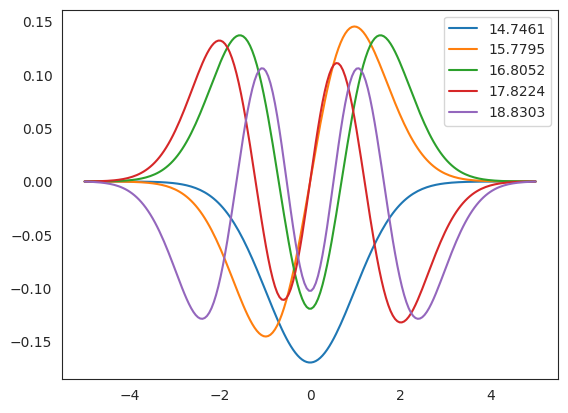
\includegraphics[width=0.9\linewidth]{fig/ks_dft_1d_wfn_ener.png}
  \caption{Wavefunction และพลังงานที่ได้จากการคำนวณ Kohn-Sham DFT สำหรับกรณี 1 มิติ}
  \label{fig:ks_dft_1d_wfn_ener}
\end{figure}

ผู้อ่านที่ต้องการศึกษาโค้ดฉบับสมบูรณ์สามารถดูได้ที่ไฟล์ \inlinehighlight{6_1D_DFT.ipynb} ใน Code Repository ของหนังสือ
\enquote{ปัญญาประดิษฐ์สำหรับเคมีควอนตัม (Machine Learning for Quantum Chemistry)} ที่
\url{https://github.com/rangsimanketkaew/ml-qm-book-code}

%----------------------------------------
\section{เขียนโปรแกรมคำนวณ Molecular Quantum Integrals }
%----------------------------------------

ในเคมีควอนตัมนั้นเราจะต้องปวดหัววุ่นวายกับการคำนวณอินทิกรัล (Integrals) ที่ถือว่าเป็นหนามยอกอกของนักเคมีเชิงฟิสิกส์สายทฤษฎีมาอย่างยาวนาน
นั่นก็คือ Molecular Integrals ที่ใช้ Gaussian Basis Functions ซึ่ง Integrals เทอมที่สำคัญ ๆ นั้นก็มีด้วยกันดังนี้

\begin{enumerate}[topsep=0pt,noitemsep]
  \item Overlap Integrals

  \item Kinetic Energy Integrals

  \item Nuclear Attraction Integrals

  \item Two-Electron Repulsion Integrals
\end{enumerate}

โดยในหัวข้อนี้ผู้อ่านจะได้เรียนรู้ทั้งทฤษฎี, อัลกอริทึม และการเขียนโปรแกรมเพื่อคำนวณเทอม Molecular Integrals ทั้ง 4 เทอม

%----------------------------------------
\subsection{ความรู้ทางคณิตศาสตร์ที่ต้องใช้}
%----------------------------------------

เริ่มต้นผมอยากจะให้ผู้อ่านได้ทำความเข้าใจคณิตศาสตร์ที่ควรจะต้องทราบก่อนที่จะไปทำความเข้าใจรายละเอียดของ Integrals โดยผมขอเริ่มด้วย
Gaussian Function แบบสามมิติ ดังนี้

\begin{equation}
  G_{ijk}(\mathbf{r}, \alpha, \mathbf{A})
  =
  x_A^i y_A^j z_A^k \hbox{exp}(-\alpha r_A^2)
\end{equation}

\noindent ซึ่งเป็นฟังก์ชันที่ขึ้นกับพารามิเตอร์ดังต่อไปนี้: Orbital Exponent $\alpha$, Electronic Coordinates $\mathbf{r}$,
Origin $\mathbf{A}$, และ

\begin{equation}
  \mathbf{r}_A
  =
  \mathbf{r} - \mathbf{A}
\end{equation}

\noindent แล้วก็ $i,j,k$ คือเลขควอนตัมเชิงมุม (Angular Quantum Numbers) เช่น $i=0$ คือ $s$-type, $i=1$ คือ $p$-type

เนื่องจากว่า Cartesian Gaussians เป็นฟังก์ชันที่ขึ้นกับทิศทาง $,x ,y, z$ ดังนั้นจึงสามารถแยกฟังก์ชันออกจากกันได้ ดังนี้

\begin{equation}
  G_{ijk}(\mathbf{r}, \alpha, \mathbf{A})
  =
  G_i(x,\alpha,A_x)G_j(y,\alpha,A_y)G_k(z,\alpha,A_z)
\end{equation}

\noindent โดยที่ฟังก์ชัน Gaussian แบบหนึ่งมิตินั้นมีสมการคือ

\begin{equation}
  G_i(x,\alpha,A_x)
  =
  (x - A_x)^i \hbox{exp}(-\alpha(x-A_x)^2)
\end{equation}

คราวนี้เรามาดู Overlap Integral ของฟังก์ชัน Gaussian แบบหนึ่งมิติ จำนวน 2 ฟังก์ชันกันครับ นั่นคือ $a$ and $b$ ดังนี้

\begin{tcolorbox}[ams align]
  S_{ab}
  &= \int G_i(x,\alpha,A_x) G_j(x,\beta,B_x) dx \\
  &= \int K_{AB} x^i_A x^j_B \hbox{exp}(-p x_P^2) dx
\end{tcolorbox}

\noindent โดยที่เราสามารถใช้คุณสมบัติการคูณของฟังก์ชัน Gaussian ได้ ดังนี้

\begin{equation}
  K_{AB}
  =
  \hbox{exp}(-q Q_x^2)
\end{equation}

\noindent ซึ่ง $q$ และ $Q$ นั้นมีนิยามดังนี้

\begin{align}
  Q_x & = A_x - B_x \quad q = \frac{\alpha\beta}{\alpha + \beta}                           \\
  p   & = \alpha + \beta \quad  \quad P_x = \frac{1}{p}\left(\alpha A_x + \beta B_x\right)
\end{align}

\noindent ถ้าหากว่าเราใช้ฟังก์ชัน Hermite Gaussians เราจะสามารถเขียน $S_{ab}$ ได้ใหม่ดังนี้

\begin{align}
  S_{ab}
   & = \int \sum\limits_{t=0}^{i+j} E_{t}^{ij} \Lambda_t dx                \\
   & = \sum\limits_{t=0}^{i+j} E_{t}^{ij} \int \Lambda_t dx                \\
   & = \sum\limits_{t=0}^{i+j} E_{t}^{ij} \delta_{t0} \sqrt{\frac{\pi}{p}} \\
   & = E_{0}^{ij} \sqrt{\frac{\pi}{p}}
\end{align}

\noindent จะเห็นว่าเราสามารถลดรูปของ Overlap Matrix $S_{ab}$ ให้ง่ายขึ้นได้โดยการใช้คุณสมบัติของ Summation และ Integral
แล้วเราก็ยังสามารถทำให้ Summation หายไปได้โดยการยุบรวม $\sum\limits_{t=0}^{i+j} E_{t}^{ij} \delta_{t0}$ เข้าด้วยกัน
แล้วเราก็มี $E_{t}^{ij}$ ซึ่งก็คือสัมประสิทธิ์การกระจาย (Expansion Coefficients) ซึ่งเราสามารถคำนวณได้โดยใช้วิธีการวนซ้ำ
และ $\Lambda_t$ คือฟัง Hermite Gaussian Overlap ระหว่างฟังก์ชัน Gaussians $a$ กับ $b$ สำหรับการคำนวณหา $E_{t}^{ij}$
เราสามารถใช้สมการต่อไปนี้

\begin{subequations}
  \begin{tcolorbox}[ams align]
    E^{ij}_t
    &= \frac{1}{2p}E^{i,j-1}_{t-1} + \frac{qQ_x}{\beta} E_{t}^{i,j-1} + (t+1) E_{t+1}^{i,j-1}
    \label{eq:expan_coeff_1} \\
    E^{ij}_t &= \frac{1}{2p}E^{i-1,j}_{t-1} - \frac{qQ_x}{\alpha} E_{t}^{i-1,j} + (t+1) E_{t+1}^{i-1,j}
    \label{eq:expan_coeff_2}
  \end{tcolorbox}
\end{subequations}

\noindent โดยสมการที่ \eqref{eq:expan_coeff_1} นั้นช่วยให้เราสามารถลดค่า Index $j$ และสมการที่ \eqref{eq:expan_coeff_2}
นั้นช่วยให้เราลดค่าของ Index $i$ ซึ่งทำให้เราได้สมการที่สั้นมากขึ้นนั่นคือสมการที่ \eqref{eq:expan_coeff_3}

\begin{subequations}
  \begin{tcolorbox}[ams gather]
    E^{00}_{0} = K_{AB} \label{eq:expan_coeff_3} \\
    E^{ij}_t = 0 \quad \hbox{ถ้า} \quad t < 0, \quad \hbox{หรือ} \quad t > i+j \label{eq:expan_coeff_4}
  \end{tcolorbox}
\end{subequations}

สรุปก็คือค่าของ $E_{t}^{ij}$ นั้นจะขึ้นอยู่กับค่าของดัชนี $i$, $j$, และ $t$ เช่น ถ้าหากว่า $i = j = t = 0$ เราก็จะได้ Expansion
Coefficient ตามสมการที่ \eqref{eq:expan_coeff_4} นั่นเอง

%----------------------------------------
\subsection{อินทิกรัลซ้อนทับ (Overlap Integrals)}
\idxth{อินทิกรัลซ้อนทับ}
\idxen{Overlap Integrals}
%----------------------------------------

อินทริกรัลอันแรกที่ผู้อ่านจะได้ศึกษาก็คือ Overlap Integrals ซึ่งเราเพิ่งดูรายละเอียดการคำนวณหาอินทิกรัลกันไปในหัวข้อที่แล้วโดยการใช้
Expansion Coefficient $E_t^{ij}$ โดยในหัวข้อนี้เราจะเริ่มด้วยการเขียนฟังก์ชัน \pyinline{E} สำหรับคำนวณ $E_t^{ij}$
ซึ่งนอกจากที่เราจะต้องรู้ค่าของ Angular Momentum $i$ และ $j$ จากฟังก์ชัน Gaussian แล้ว เรายังจะต้องรู้ค่าของระยะห่างระหว่าง Gaussian
Function $Q_x$ ด้วย รวมถึงค่าของ Orbital Exponent Coefficients $\alpha$ กับ $\beta$

\vspace{5pt}

\begin{lstlisting}[style=MyPython]
def E(i, j, t, Qx, a, b):
    """
    Recursive definition of Hermite Gaussian coefficients.

    Returns a float.
    a: orbital exponent on Gaussian 'a' (e.g. alpha in the text)
    b: orbital exponent on Gaussian 'b' (e.g. beta in the text)
    i,j: orbital angular momentum number on Gaussian 'a' and 'b'
    t: number nodes in Hermite (depends on type of integral,
        e.g. always zero for overlap integrals)
    Qx: distance between origins of Gaussian 'a' and 'b'
    """
    p = a + b
    q = a * b / p
    if (t < 0) or (t > (i + j)):
        # out of bounds for t
        return 0.0
    elif i == j == t == 0:
        # base case
        return np.exp(-q * Qx * Qx)  # K_AB
    elif j == 0:
        # decrement index i
        return (
            (1 / (2 * p)) * E(i - 1, j, t - 1, Qx, a, b)
            - (q * Qx / a) * E(i - 1, j, t, Qx, a, b)
            + (t + 1) * E(i - 1, j, t + 1, Qx, a, b)
        )
    else:
        # decrement index j
        return (
            (1 / (2 * p)) * E(i, j - 1, t - 1, Qx, a, b)
            + (q * Qx / b) * E(i, j - 1, t, Qx, a, b)
            + (t + 1) * E(i, j - 1, t + 1, Qx, a, b)
        )
\end{lstlisting}

\vspace{5pt}

จะเห็นว่าสำหรับ Overlap แบบหนึ่งมิติ (1D) ระหว่าง Gaussian Function 2 อันนั้น เราก็แค่ทำการคำนวณ $E_0^{ij}$ แล้วก็คูณด้วย
$\sqrt{\frac{\pi}{p}}$ แล้วก็ถ้าเป็นแบบสามมิติ (3D) เราก็แค่นำ Overlap แบบ 1D สำหรับ $x,y,z$ มาคูณเข้าด้วยกัน
ดังนั้น เราสามารถเขียนโค้ดสำหรับการคำนวณ 3D Overlap ได้ดังนี้

\vspace{5pt}

\begin{lstlisting}[style=MyPython]
import numpy as np


def overlap(a, lmn1, A, b, lmn2, B):
    """
    Evaluates overlap integral between two Gaussians

    Returns a float.
    a: orbital exponent on Gaussian 'a' (e.g. alpha in the text)
    b: orbital exponent on Gaussian 'b' (e.g. beta in the text)
    lmn1: int tuple containing orbital angular momentum (e.g. (1,0,0))
          for Gaussian 'a'
    lmn2: int tuple containing orbital angular momentum for Gaussian 'b'
    A: list containing origin of Gaussian 'a', e.g. [1.0, 2.0, 0.0]
    B: list containing origin of Gaussian 'b'
    """
    l1, m1, n1 = lmn1  # shell angular momentum on Gaussian 'a'
    l2, m2, n2 = lmn2  # shell angular momentum on Gaussian 'b'
    S1 = E(l1, l2, 0, A[0] - B[0], a, b)  # X
    S2 = E(m1, m2, 0, A[1] - B[1], a, b)  # Y
    S3 = E(n1, n2, 0, A[2] - B[2], a, b)  # Z

    return S1 * S2 * S3 * np.power(np.pi / (a + b), 1.5)
\end{lstlisting}

\vspace{5pt}

เราใช้ไลบรารี่ NumPy เพื่อที่ว่าเราสามารถใช้ค่าคงที่ของ $\pi$ และเลขกกำลังแบบเศษส่วน $(3/2)$ ได้นั่นเอง แล้วก็การเขียนฟังก์ชันด้านบน
ท\pyinline{overlap} และ \pyinline{E} ทั้งสองอันนั้นก็เพียงพอแล้วต่อการคำนวณหา Overlap Integrals ระหว่าง Gaussian Function
แบบที่เป็น Primitive แต่ประเด็นก็คือว่า Basis Functions ส่วนใหญ่ในการคำนวณทางควอนตัมนั้นเป็นแบบ Contracted Basis Functions
นั่นก็คือเป็น Basis Function ที่เกิดจากการรวมเอา Gaussian Primitive Function หลาย ๆ อันมารวมกัน ซึ่งจริง ๆ ถ้าหากว่าเราจะต้องหา
Overlap Integrals ระหว่าง Contracted Gaussian Function นั้นก็ทำได้ไม่ยาก โดยสามารถดูได้ในฟังก์ชัน \pyinline{S(a,b)} ดังนี้

\vspace{5pt}

\begin{lstlisting}[style=MyPython]
def S(a, b):
    """
    Evaluates overlap between two contracted Gaussians

    Returns float.
    Arguments:
    a: contracted Gaussian 'a', BasisFunction object
    b: contracted Gaussian 'b', BasisFunction object
    """
    s = 0.0
    for ia, ca in enumerate(a.coefs):
        for ib, cb in enumerate(b.coefs):
            s += (
                a.norm[ia]
                * b.norm[ib]
                * ca
                * cb
                * overlap(a.exps[ia], a.shell, a.origin, b.exps[ib], b.shell, b.origin)
            )

    return s
\end{lstlisting}

\vspace{5pt}

เมื่อเราได้ฟังก์ชัน \pyinline{S(a,b)} แล้ว สิ่งที่เราจะทำต่อไปก็คือเราจะมาลองทดสอบคำนวณค่าของ $S$ กันครับ โดยเราจะลองคำนวณหา $S$
ของ Basis Function 2 อันที่เหมือนกัน ซึ่งคำตอบที่เราจะต้องได้ออกมานั้นแน่นอนว่าจะต้องเท่ากับ 1 เพราะว่าฟังก์ชันที่เหมือนกันก็จะ Overlap
กันได้พอดี โดยเราจะต้องมาเขียนโค้ดสำหรับสร้าง Basis Function กันก่อน โดยเราจะใช้ \pyinline{class} สำหรับ \pyinline{BasisFunction}
แล้วเราก็จะใช้ \pyinline{class} ดังกล่าวในการสร้าง Object ที่จะมีข้อมูลของ  Basis Function เป็นจำนวนหลาย ๆ อัน
โดยโค้ดที่เราจะเขียนนั้นจะอ้างอิงตามสมการต่อไปนี้\footnote{ดูรายละเอียดการพิสูจน์ได้ที่ Fundamentals of Molecular Integrals Evaluation
  โดย Justin T. Fermann และ Edward F. Valeev\autocite{fermann2020}}

เริ่มด้วย Self-Overlap Integral คือ

\begin{equation}
  \int \phi^*(\mathbf{r}) \phi(\mathbf{r}) d \mathbf{r}
  =
  \frac{N^2 \pi^{3 / 2}(2 l-1) ! !(2 m-1) ! !(2 n-1) ! !}{2^{l+m+n}}
  \sum_{i, j}^n \frac{a_i a_j}{\left(\alpha_i+\alpha_j\right)^{l+m+n+3 / 2}}
\end{equation}

\noindent เนื่องจากว่า $l + m + n = L$ (โมเมนตัมเชิงมุมของแต่ละชั้น (Shell)) เราจะสามารถปรับสมการเพื่อคำนวณหา Normalization
Factor $N$ ได้ดังนี้

\begin{align}
  \int \phi^* \phi
   & =
  \frac{N^2 \pi^{3 / 2}(2 l-1) ! !(2 m-1) ! !(2 n-1) ! !}{2^L}
  \sum_{i, j}^n \frac{a_i a_j}{\left(\alpha_i+\alpha_j\right)^{L+3 / 2}} \\
   & =
  1
\end{align}

\begin{equation}
  N
  =
  \left[
    \frac{\pi^{3 / 2}(2 l-1) ! !(2 m-1) ! !(2 n-1) ! !}{2^L}
    \sum_{i, j}^n \frac{a_i a_j}{\left(\alpha_i+\alpha_j\right)^{L+3 / 2}}
    \right]^{-1 / 2}
\end{equation}

\noindent แล้วเราก็จะสามารถเขียนโค้ดเพื่อ Implement สมการที่ ได้ดังนี้

\vspace{5pt}

\begin{lstlisting}[style=MyPython]
from scipy.special import factorial2 as fact2


class BasisFunction(object):
    """
    A class that contains all our basis function data

    Attributes:
    origin: array/list containing the coordinates of the Gaussian origin
    shell: tuple of angular momentum
    exps: list of primitive Gaussian exponents
    coefs: list of primitive Gaussian coefficients
    norm: list of normalization factors for Gaussian primitives
    """

    def __init__(self, origin=[0.0, 0.0, 0.0], shell=(0, 0, 0), exps=[], coefs=[]):
        self.origin = np.asarray(origin)
        self.shell = shell
        self.exps = exps
        self.coefs = coefs
        self.norm = None
        self.normalize()

    def normalize(self):
        """
        Routine to normalize the basis functions,
        in case they do not integrate to unity.
        """
        l, m, n = self.shell
        L = l + m + n
        # self.norm is a list of length equal to number primitives
        # normalize primitives first (PGBFs)
        self.norm = np.sqrt(
            np.power(2, 2 * (l + m + n) + 1.5)
            * np.power(self.exps, l + m + n + 1.5)
            / fact2(2 * l - 1)
            / fact2(2 * m - 1)
            / fact2(2 * n - 1)
            / np.power(np.pi, 1.5)
        )

        # now normalize the contracted basis functions (CGBFs)
        # Eq. 1.44 of Valeev integral whitepaper
        prefactor = (
            np.power(np.pi, 1.5)
            * fact2(2 * l - 1)
            * fact2(2 * m - 1)
            * fact2(2 * n - 1)
            / np.power(2.0, L)
        )

        N = 0.0
        num_exps = len(self.exps)
        for ia in range(num_exps):
            for ib in range(num_exps):
                N += (
                    self.norm[ia]
                    * self.norm[ib]
                    * self.coefs[ia]
                    * self.coefs[ib]
                    / np.power(self.exps[ia] + self.exps[ib], L + 1.5)
                )

        N *= prefactor
        N = np.power(N, -0.5)
        for ia in range(num_exps):
            self.coefs[ia] *= N
\end{lstlisting}

\vspace{5pt}

ถ้าหากว่าเรามี Basis Function STO-3G ของออร์บิทัล $1s$ ของไฮโดรเจนที่มีจุดกำเนิดอยู่ที่ $(1.0, 2.0, 3.0)$ เราจะสามารถสร้าง Basis
Function ได้ดังนี้

\vspace{5pt}

\begin{lstlisting}[style=MyPython]
myOrigin = [1.0, 2.0, 3.0]
myShell = (0, 0, 0)  # p-orbitals would be (1,0,0) or (0,1,0) or (0,0,1), etc.
myExps = [3.42525091, 0.62391373, 0.16885540]
myCoefs = [0.15432897, 0.53532814, 0.44463454]
a = BasisFunction(origin=myOrigin, shell=myShell, exps=myExps, coefs=myCoefs)
\end{lstlisting}

\vspace{5pt}

\noindent โดยข้อมูลของ Basis Function ด้านบนนั้นสามารถดูได้จาก STO-3G ของ EMSL Basis Set Exchange Library ดังนี้

\vspace{5pt}

\begin{lstlisting}
!  STO-3G  EMSL  Basis Set Exchange Library 
! Elements                             References
! --------                             ----------
!  H - Ne: W.J. Hehre, R.F. Stewart and J.A. Pople, J. Chem. Phys. 2657 (1969).

****
H     0 
S   3   1.00
      3.42525091             0.15432897       
      0.62391373             0.53532814       
      0.16885540             0.44463454       
****
\end{lstlisting}

\vspace{5pt}

ดังนั้น $S(a,a) = 1.0$ เนื่องจากว่าการ Overlap ของ Basis Function กับตัวมันเองนั้นมีค่าเท่ากับ 1 เพราะว่าเราได้มีการใช้ Normalized
Factor $N$ ด้วยนั่นเอง

%----------------------------------------
\subsection{อินทิกรัลพลังงานจลน์ (Kinetic Energy Integrals)}
\idxth{อินทิกรัลพลังงานจลน์}
\idxen{Kinetic Energy Integrals}
%----------------------------------------

เรามาต่อกันที่อินทิกรัลอันที่สองนั่นก็คือ อินทิกรัลพลังงานจลน์ (Kinetic Energy Integrals) ซึ่งสามารถเขียนได้ในรูปของอินทิกรัลซ้อนทับ
(Overlap Integral) ดังนี้\footnote{นั่นจึงเป็นเหตุผลที่ว่าทำไมเราถึงต้องดูรายละเอียดของ OVerlap Integral เป็นอันดับแรก
  เพราะว่าเป็นอินทิกรัลสำคัญที่เรานำไปใช้ในการคำนวณอินทิกรัลหรือเทอมอื่น ๆ ในวิชาโครงสร้างเชิงอิเล็กทรอนิกส์}

\begin{equation}
  T_{ab}
  =
  -\frac{1}{2}\left[P_{ij}^2 S_{kl} S_{mn} + S_{ij}P_{kl}^2 S_{mn} + S_{ij} S_{kl} P_{mn}^2\right]
\end{equation}

where

\begin{equation}
  D_{ij}^2
  =
  j(j-1)S_{i,j-2} - 2\beta(2j +1)S_{ij} + 4\beta^2 S_{i,j+2}
\end{equation}

สำหรับ Primitive Function แบบ 3D เราสามารถสร้างฟังก์ชันสำหรับคำนวณ Kinetic Integral ได้คล้าย ๆ กันกับฟังก์ชันของ Overlap
Integral ดังนี้

\vspace{5pt}

\begin{lstlisting}[style=MyPython]
def kinetic(a, lmn1, A, b, lmn2, B):
    """
    Evaluates kinetic energy integral between two Gaussians

    Returns a float.
    a: orbital exponent on Gaussian 'a' (e.g. alpha in the text)
    b: orbital exponent on Gaussian 'b' (e.g. beta in the text)
    lmn1: int tuple containing orbital angular momentum (e.g. (1,0,0))
          for Gaussian 'a'
    lmn2: int tuple containing orbital angular momentum for Gaussian 'b'
    A: list containing origin of Gaussian 'a', e.g. [1.0, 2.0, 0.0]
    B: list containing origin of Gaussian 'b'
    """
    l1, m1, n1 = lmn1
    l2, m2, n2 = lmn2
    term0 = (
        b * (2 * (l2 + m2 + n2) + 3) * overlap(a, (l1, m1, n1), A, b, (l2, m2, n2), B)
    )
    term1 = (
        -2
        * np.power(b, 2)
        * (
            overlap(a, (l1, m1, n1), A, b, (l2 + 2, m2, n2), B)
            + overlap(a, (l1, m1, n1), A, b, (l2, m2 + 2, n2), B)
            + overlap(a, (l1, m1, n1), A, b, (l2, m2, n2 + 2), B)
        )
    )
    term2 = -0.5 * (
        l2 * (l2 - 1) * overlap(a, (l1, m1, n1), A, b, (l2 - 2, m2, n2), B)
        + m2 * (m2 - 1) * overlap(a, (l1, m1, n1), A, b, (l2, m2 - 2, n2), B)
        + n2 * (n2 - 1) * overlap(a, (l1, m1, n1), A, b, (l2, m2, n2 - 2), B)
    )
    return term0 + term1 + term2
\end{lstlisting}

\vspace{5pt}

\noindent และสำหรับ Contracted Gaussian Functions เราสามารถเขียนฟังก์ชัน \pyinline{T(a,b)} ได้ดังนี้

\vspace{5pt}

\begin{lstlisting}[style=MyPython]
def T(a, b):
    """
    Evaluates kinetic energy between two contracted Gaussians

    Returns float.
    Arguments:
    a: contracted Gaussian 'a', BasisFunction object
    b: contracted Gaussian 'b', BasisFunction object
    """
    t = 0.0
    for ia, ca in enumerate(a.coefs):
        for ib, cb in enumerate(b.coefs):
            t += (
                a.norm[ia]
                * b.norm[ib]
                * ca
                * cb
                * kinetic(a.exps[ia], a.shell, a.origin, b.exps[ib], b.shell, b.origin)
            )
    return t
\end{lstlisting}

%----------------------------------------
\subsection{อินทิกรัลแรงดึงดูดเชิงนิวเคลียร์ (Nuclear Attraction Integrals)}
\idxth{อินทิกรัลแรงดึงดูดเชิงนิวเคลียร์}
\idxen{Nuclear Attraction Integrals}
%----------------------------------------

ในหัวข้อนี้เราจะมาดูรายละเอียดของอินทิกรัลอีกอันหนึ่งซึ่งเป็น One-Body Integral นั่นคืออินทิกรัลแรงดึงดูดเชิงนิวเคลียร์ (Nuclear Attraction
Integrals) โดยอินทิกรัลอันนี้จะแตกต่างจาก Overlap Integral และ Kinetic Integral ตรงที่เรามีการใช้โอเปอร์เรเตอร์ $1/r_C$
ซึ่งก็คือคูลอมป์ นั่นหมายความว่าเราไม่สามารถทำการแยกตัวประกอบ (Factorization) อินทิกรัลของเราให้อยู่ในรูปของพิกัดคาร์ทีเซียน
(Cartesian Components) หรือ $x,y,z$ ได้นั่นเอง ดังนั้นในการคำนวณ Nuclear Attraction Integral เราจำเป็นต้องใช้ตัวช่วยนั่นก็คือ
Hermite Coulomb Integral $(R^n_{tuv}(p,\mathbf{P},\mathbf{C}))$ ซึ่งเป็นตัวแทนของอันตรกิริยาแบบคูลอมป์ (Coulomb Interaction)
ที่เกิดขึ้นระหว่างการกระจายตัวของประจุแบบ Gaussian ในโมเลกุลซึ่งมีจุดศูนย์กลางคือ $\mathbf{P}$ ส่วนนิวเคลียสนั้นมีจุดศูนย์กลางอยู่ที่
$\mathbf{C}$ โดย Hermite Coulomb Integral นั้นมีองค์ประกอบคือ $E_t^{ij}$ ซึ่งสามารถหาได้ด้วยวิธีการวนซ้ำตามชุดสมการดังต่อไปนี้

\begin{align}
  R^{n}_{t+1,u,v} & = t R^{n+1}_{t-1,u,v} + X_{PC}R^{n+1}_{t,u,v} \\
  R^{n}_{t,u+1,v} & = u R^{n+1}_{t,u-1,v} + Y_{PC}R^{n+1}_{t,u,v} \\
  R^{n}_{t,u,v+1} & = v R^{n+1}_{t,u,v-1} + Z_{PC}R^{n+1}_{t,u,v} \\
  R^{n}_{0,0,0}   & = (-2p)^n F_n (p R_{PC}^2)
\end{align}

\noindent โดยที่ $F_n(T)$ คือฟังก์ชันของบอยส์ (Boys Function)

\begin{equation}
  F_n(T)
  =
  \int_0^1 \hbox{exp}(-Tx^2)x^{2n}dx
\end{equation}

\noindent ซึ่ง Boys Function นั้นเป็นกรณีเฉพาะแบบพิเศษของ Kummer Confluent Hypergeometric Function $_1F_1(a,b,x)$
ดังนี้\footnote{\url{https://en.wikipedia.org/wiki/Confluent_hypergeometric_function}}

\begin{equation}
  F_n(T)
  =
  \frac{_1F_1(n+\frac{1}{2}, n+\frac{3}{2}, -T)}{2n+1}
\end{equation}

\noindent โดยที่เราสามารถ Implement สมการด้านบนนี้ได้ง่าย ๆ โดยการใช้ฟังก์ชันของไลบรารี่ \pyinline{SciPy} สำหรับ $_1F_1$
ซึ่งอยู่ในโมดูล \pyinline{scipy.special}

\vspace{5pt}

\begin{lstlisting}[style=MyPython]
def R(t, u, v, n, p, PCx, PCy, PCz, RPC):
    """
    Returns the Coulomb auxiliary Hermite integrals

    Returns a float.
    Arguments:
    t,u,v: order of Coulomb Hermite derivative in x,y,z
           (see defs in Helgaker and Taylor)
    n: order of Boys function
    PCx,y,z: Cartesian vector distance between Gaussian
             composite center P and nuclear center C
    RPC: Distance between P and C
    """
    T = p * RPC * RPC
    val = 0.0
    if t == u == v == 0:
        val += np.power(-2 * p, n) * boys(n, T)
    elif t == u == 0:
        if v > 1:
            val += (v - 1) * R(t, u, v - 2, n + 1, p, PCx, PCy, PCz, RPC)
        val += PCz * R(t, u, v - 1, n + 1, p, PCx, PCy, PCz, RPC)
    elif t == 0:
        if u > 1:
            val += (u - 1) * R(t, u - 2, v, n + 1, p, PCx, PCy, PCz, RPC)
        val += PCy * R(t, u - 1, v, n + 1, p, PCx, PCy, PCz, RPC)
    else:
        if t > 1:
            val += (t - 1) * R(t - 2, u, v, n + 1, p, PCx, PCy, PCz, RPC)
        val += PCx * R(t - 1, u, v, n + 1, p, PCx, PCy, PCz, RPC)
    return val
\end{lstlisting}

\vspace{5pt}

\noindent และเราสามารถทำการกำหนด Boys Function โดยการเขียนฟังก์ชัน \pyinline{boys(n,T)} ได้ดังนี้

\vspace{5pt}

\begin{lstlisting}[style=MyPython]
from scipy.special import hyp1f1

def boys(n, T):
    return hyp1f1(n + 0.5, n + 1.5, -T) / (2.0 * n + 1.0)
\end{lstlisting}

\vspace{5pt}

\noindent แล้วเราก็สามารถคำนวณ $\mathbf{P}$ ได้โดยการใช้ Gaussian Product Center Rule ดังนี้

\begin{equation}
  P
  =
  \frac{\alpha A + \beta B}{\alpha + \beta}
\end{equation}

\noindent ซึ่งสามารถเขียนออกมาเป็นโค้ดได้ง่าย ๆ ดังนี้

\vspace{5pt}

\begin{lstlisting}[style=MyPython]
def gaussian_product_center(a, A, b, B):
    return (a * A + b * B) / (a + b)
\end{lstlisting}

\vspace{5pt}

เมื่อเราคำนวณ Coulomb Auxiliary Hermite Integrals $R^{n}_{tuv}$ ออกมาได้แล้ว ขั้นตอนต่อไปคือเราสามารถคำนวณ Nuclear
Attraction Integral โดยเทียบกับนิวเคลียสที่มีจุดศูนย์กลางอยู่ที่ $\mathbf{C}$, $V_{ab}(C)$ ได้โดยการใช้สมการต่อไปนี้
expression

\begin{equation}
  V_{ab}(C)
  =
  \frac{2\pi}{p}
  \sum\limits_{t,u,v}^{\substack{i+j+1,\\k+l+1,\\m+n+1}}
  E_t^{ij} E_u^{kl} E_v^{mn} R^0_{tuv}(p,\mathbf{P},\mathbf{C})
\end{equation}

\noindent ซึ่งเราก็จะสามารถ Implement สมการด้านบนนี้ให้เป็นโค้ดตามฟังก์ชัน \pyinline{nuclear_attraction} ได้ดังนี้

\vspace{5pt}

\begin{lstlisting}[style=MyPython]
def nuclear_attraction(a, lmn1, A, b, lmn2, B, C):
    """
    Evaluates kinetic energy integral between two Gaussians

    Returns a float.
    a: orbital exponent on Gaussian 'a' (e.g. alpha in the text)
    b: orbital exponent on Gaussian 'b' (e.g. beta in the text)
    lmn1: int tuple containing orbital angular momentum (e.g. (1,0,0))
          for Gaussian 'a'
    lmn2: int tuple containing orbital angular momentum for Gaussian 'b'
    A: list containing origin of Gaussian 'a', e.g. [1.0, 2.0, 0.0]
    B: list containing origin of Gaussian 'b'
    C: list containing origin of nuclear center 'C'
    """
    l1, m1, n1 = lmn1
    l2, m2, n2 = lmn2
    p = a + b
    P = gaussian_product_center(a, A, b, B)  # Gaussian composite center
    RPC = np.linalg.norm(P - C)

    val = 0.0
    for t in range(l1 + l2 + 1):
        for u in range(m1 + m2 + 1):
            for v in range(n1 + n2 + 1):
                val += (
                    E(l1, l2, t, A[0] - B[0], a, b)
                    * E(m1, m2, u, A[1] - B[1], a, b)
                    * E(n1, n2, v, A[2] - B[2], a, b)
                    * R(t, u, v, 0, p, P[0] - C[0], P[1] - C[1], P[2] - C[2], RPC)
                )
    val *= 2 * np.pi / p
    return val
\end{lstlisting}

\vspace{5pt}

\noindent และเราก็สามารถใช้ Contracted Gaussians ในการคำนวณอินทิกรัลของเราได้ตามที่แสดงในโค้ดดังต่อไปนี้

\vspace{5pt}

\begin{lstlisting}[style=MyPython]
def V(a, b, C):
    """
    Evaluates overlap between two contracted Gaussians

    Returns float.
    Arguments:
    a: contracted Gaussian 'a', BasisFunction object
    b: contracted Gaussian 'b', BasisFunction object
    C: center of nucleus
    """
    v = 0.0
    for ia, ca in enumerate(a.coefs):
        for ib, cb in enumerate(b.coefs):
            v += (
                a.norm[ia]
                * b.norm[ib]
                * ca
                * cb
                * nuclear_attraction(
                    a.exps[ia], a.shell, a.origin, b.exps[ib], b.shell, b.origin, C
                )
            )
    return v
\end{lstlisting}

\vspace{5pt}

ผู้อ่านจะต้องเข้าใจด้วยว่าอินทิกรัลที่เราคำนวณออกมาได้นั้นเป็นแค่ Nuclear Attraction เท่านั้น ซึ่งเรายังมี Nuclear Repulsion Integrals
ที่เป็น Contribution มาจากอะตอมที่มีจุดศูนย์กลางอยู่ที่ $\mathbf{C}$ อีกด้วย ถ้าหากว่าเราต้องการคำนวณ Nuclear Attraction Contribution
ทั้งหมดของทั้งโมเลกุล เราจะต้องทำการรวม Integral ทั้งหมดทุกเทอมของทุกอะตอมเข้าด้วยแล้วก็ทำตามปรับสเกลของแต่ละ Integral ตามประจุย่อย
(Nuclear Charge) ของอะตอมนั้น ๆ

%----------------------------------------
\subsection{อินทิกรัลแรงผลักระหว่างอิเล็กตรอน (Two-Electron Repulsion Integrals)}
\idxth{อินทิกรัลแรงผลักระหว่างอิเล็กตรอน}
\idxen{Two-Electron Repulsion Integrals}
%----------------------------------------

เราได้ดูรายละเอียดของ One-Body Integrals ไปครับแล้ว ซึ่งเป็นอินทิกรัลพื้นฐานที่ผู้อ่านควรจะต้องทราบหากต้องการเขียนโปรแกรมสำหรับคำนวณ%
พลังงานของโมเลกุลด้วยวิธี Hartree-Fock ในหัวข้อเราจะมาดูรายละเอียดของอินทิกรัลอันสุดท้ายซึ่งเป็นอินทิกรัลที่สำคัญมากและมีความซับซ้อนมากเช่นกัน
นั่นคือ Electron-Electron Repulsion Integrals หรืออินทิกรัลของแรงผลักระหว่างอิเล็กตรอน ซึ่งเป็นอินทิกรัลแบบ Two-Body

ในการคำนวณหาอินทิกรัลอันนี้นั้น เราจะยังคงมีการใช้ Hermite Integrals ซึ่งเราจะต้องทำการหาผลรวมดังต่อไปนี้

\begin{equation}
  \begin{aligned}
    g_{abcd}
    =
     & \frac{2\pi^{5/2}}{pq\sqrt{p+q}}              \\
     & \sum\limits_{t,u,v}^{\substack{i+j+1,        \\k+l+1, \\m+n+1}}
    E_t^{ij}
    E_u^{kl}
    E_v^{mn}
    \sum\limits_{\tau,\nu,\phi}^{\substack{i'+j'+1, \\k'+l'+1, \\m'+n'+1}}
    E_{\tau}^{i'j'}
    E_{\nu}^{k'l'}
    E_{\phi}^{m'n'}
    (-1)^{\tau+\nu+\phi}
    R^0_{t+\tau, u + \nu, v+\phi}(p,q,\mathbf{P},\mathbf{Q})
  \end{aligned}
\end{equation}

\noindent ซึ่งจะเห็นได้ว่าสมการด้านบนนี้น่ากลัวมาก มีความซับซ้อนมาก อย่างไรก็ตาม เนื่องจากว่าเราทราบว่า $p = \alpha + \beta$
เราจะกำหนดให้ $q = \gamma + \delta$ เพื่อที่ว่าเราจะได้มี Gaussian Function Exponents ของ $a$, $b$, $c$ และ $d$
ซึ่งเราสามารถเขียนสมการใหม่อีกสมการที่มีหน้าตาคล้าย ๆ กับ Nuclear Attraction Integrals ได้ดังนี้

\vspace{5pt}

\begin{lstlisting}[style=MyPython]
def electron_repulsion(a, lmn1, A, b, lmn2, B, c, lmn3, C, d, lmn4, D):
    """
    Evaluates kinetic energy integral between two Gaussians

    Returns a float.
    a,b,c,d: orbital exponent on Gaussian 'a','b','c','d'
    lmn1,lmn2
    lmn3,lmn4: int tuple containing orbital angular momentum
               for Gaussian 'a','b','c','d', respectively
    A,B,C,D: list containing origin of Gaussian 'a','b','c','d'
    """
    l1, m1, n1 = lmn1
    l2, m2, n2 = lmn2
    l3, m3, n3 = lmn3
    l4, m4, n4 = lmn4
    p = a + b  # composite exponent for P (from Gaussians 'a' and 'b')
    q = c + d  # composite exponent for Q (from Gaussians 'c' and 'd')
    alpha = p * q / (p + q)
    P = gaussian_product_center(a, A, b, B)  # A and B composite center
    Q = gaussian_product_center(c, C, d, D)  # C and D composite center
    RPQ = np.linalg.norm(P - Q)

    val = 0.0
    for t in range(l1 + l2 + 1):
        for u in range(m1 + m2 + 1):
            for v in range(n1 + n2 + 1):
                for tau in range(l3 + l4 + 1):
                    for nu in range(m3 + m4 + 1):
                        for phi in range(n3 + n4 + 1):
                            val += (
                                E(l1, l2, t, A[0] - B[0], a, b)
                                * E(m1, m2, u, A[1] - B[1], a, b)
                                * E(n1, n2, v, A[2] - B[2], a, b)
                                * E(l3, l4, tau, C[0] - D[0], c, d)
                                * E(m3, m4, nu, C[1] - D[1], c, d)
                                * E(n3, n4, phi, C[2] - D[2], c, d)
                                * np.power(-1, tau + nu + phi)
                                * R(
                                    t + tau,
                                    u + nu,
                                    v + phi,
                                    0,
                                    alpha,
                                    P[0] - Q[0],
                                    P[1] - Q[1],
                                    P[2] - Q[2],
                                    RPQ,
                                )
                            )

    val *= 2 * np.power(np.pi, 2.5) / (p * q * np.sqrt(p + q))
    return val
\end{lstlisting}

\vspace{5pt}

\noindent และเพื่อให้มีความสมบูรณ์มากกว่านี้ เราจะสามารถเขียนฟังก์ชันเพื่อคำนวณหา Electron-Electron Respulsion Integral
สำหรับ Contracted Gaussians ได้ดังนี้

\vspace{5pt}

\begin{lstlisting}[style=MyPython]
def ERI(a, b, c, d):
    """
    Evaluates overlap between two contracted Gaussians

    Returns float.
    Arguments:
    a: contracted Gaussian 'a', BasisFunction object
    b: contracted Gaussian 'b', BasisFunction object
    c: contracted Gaussian 'b', BasisFunction object
    d: contracted Gaussian 'b', BasisFunction object
    """
    eri = 0.0
    for ja, ca in enumerate(a.coefs):
        for jb, cb in enumerate(b.coefs):
            for jc, cc in enumerate(c.coefs):
                for jd, cd in enumerate(d.coefs):
                    eri += (
                        a.norm[ja]
                        * b.norm[jb]
                        * c.norm[jc]
                        * d.norm[jd]
                        * ca
                        * cb
                        * cc
                        * cd
                        * electron_repulsion(
                            a.exps[ja],
                            a.shell,
                            a.origin,
                            b.exps[jb],
                            b.shell,
                            b.origin,
                            c.exps[jc],
                            c.shell,
                            c.origin,
                            d.exps[jd],
                            d.shell,
                            d.origin,
                        )
                    )
    return eri
\end{lstlisting}

\vspace{5pt}

ทั้งหมดที่เราเพิ่งดูรายละเอียดกันไปนั้นคือสมการและการเขียนโค้ดของอินทิกรัลทั้งหมดที่จำเป็นต้องใช้ในการเขียนโปรแกรมเคมีควอนตัมด้วยวิธี
Hartree-Fock นั่นเองครับ

%----------------------------------------
\subsection{การพิจารณาประสิทธิภาพเชิงการคำนวณ (Computational Efficiency)}
%----------------------------------------

จากที่เราได้ศึกษา Integrals แบบต่าง ๆ มาแล้วทั้งสมการคณิตศาสตร์และการเขียนโปรแกรม ผู้อ่านจะพบว่าโค้ดที่ผมเอามาให้ดูเป็นตัวอย่างนั้น%
สามารถทำงานได้ปกติ ได้ผลการคำนวณที่ถูกต้อง แต่ประเด็นสำคัญอีกอย่างหนึ่งก็คือเรื่องของประสิทธิภาพของโปรแกรมหรือโค้ด แน่นอนว่าโค้ดของเรา%
รันได้ แต่ว่าจะโค้ดจะทำงานได้ช้าหรือเร็วนั้นก็ขึ้นอยู่กับว่าเราเขียนโค้ดอย่างไร นอกจากนี้ยังขึ้นกับภาษาคอมพิวเตอร์ที่เราใช้ในการเขียนด้วย
โดยภาษาที่ผมเลือกมาใช้ในการเขียนโค้ดในหนังสือเล่มนี้นั้นส่วนใหญ่เป็นภาษา Python เพราะว่าเขียนได้ง่าย ผู้อ่านสามารถศึกษาตามได้ไม่ยาก%
เมื่อเทียบกับภาษาอื่น ๆ

ถ้าหากว่าเราเขียนโค้ดออกมาแล้วนำไปใช้เลยโดยที่ไม่มีพิจารณาประสิทธิภาพเชิงการคำนวณก่อนนั้น โค้ดของเราก็อาจจะไม่สามารถทำงานได้เต็มที่%
บนคอมพิวเตอร์ที่มีประสิทธิภาพสูง เช่น Supercomputer ดังนั้นเราจะมาดูกันว่าเราจะสามารถปรับปรุงโค้ดของเราได้อย่างไรบ้างเพื่อที่ว่าจะสามารถนำ%
ไปใช้ได้จริง

ปัจจัยแรกเลยคือภาษาคอมพิวเตอร์ที่เรานำมาใช้ในการเขียนโค้ด จริง ๆ แล้วถ้าหากว่าเราอยากจะเขียนโค้ดแบบจริงจังเพื่อให้ทำงานได้อย่างมีประสิทธิภาพ
เราไม่ควรเขียนโปรแกรมโดยการใช้เพียงแค่ภาษา Python เพราะว่าภาษา Python นั้นจะทำงานได้ช้ากว่าภาษาคอมพิวเตอร์อื่นที่เป็นแบบ Low-Level
เหตุผลที่โค้ดของเราด้านบนที่ถูกด้วยเขียน Python ทำงานได้ช้านั้นก็เพราะว่าเรามีการวนลูปโดยการใช้ \pyinline{for} แบบหลาย ๆ ชั้น (Nested
Loop) ซึ่งเป็นตัวการที่ทำให้โค้ดของเราช้า ดังนั้นจึงจะเป็นการดีกว่าถ้าหากว่าเราเขียนบางส่วนของโค้ด Python ของเราด้วยเทคนิคต่าง ๆ
โดยหนึ่งในนั้นก็คือการเขียนโค้ดใหม่ด้วย Cython (\url{http://www.cython.org}) ซึ่งจะช่วยให้โค้ดของเราทำงานได้เร็วขึ้นหลายสิบเท่าเลย
ปัญหาอีกอย่างหนึ่งของ Python ก็คือมีการใช้ Global Interpreter Lock (GIL) ซึ่งทำให้เราไม่สามารถรันโค้ดของเราแบบขนาน (Parallel) ได้
ซึ่งถ้าหากว่าเราสามารถทำการแบ่ง Routine ในโค้ดการคำนวณ Integral ของเราออกเป็นหลาย ๆ อันและทำการรัน Routines เหล่านั้นด้วย
CPUs หลาย ๆ อันได้ก็จะทำให้โค้ดเราทำงานได้เร็วขึ้นเยอะมาก โดยหนึ่งในวิธีการเขียนโค้ดแบบ Parallel นั้นก็คือการใช้วิธี OpenMP
หรือใช้โมดูลของ Cython นั่นคือ \pyinline{cython.parallel} โดยผู้อ่านสามารถนำเทคนิคเหล่านี้ไปใช้ในการทำให้โค้ดการคำนวณ Integrals
ของเราได้ เช่น หลีกเลี่ยงการคำนวณแบบวนซ้ำหลาย ๆ รอบ (Explicit Recursion) ในฟังก์ชัน \pyinline{E} และ \pyinline{R}

นอกจากนี้ผู้อ่านยังสามารถใช้เทคนิคอื่น ๆ ได้อีก เช่น ใช้ Permutational Symmetry ของอินทิกรัล เช่น เราสามารถทำการคำนวณ Two-Electron
Repulsion Integral ได้เร็วขึ้นประมาณ 8 เท่าเพียงแค่นำคุณสมบัติของความสมมาตรของอินทิกรัลมาใช้ แล้วเราก็สามารถหลักเลี่ยงการคำนวณ
Integrals หลาย ๆ อันที่มีค่าเท่ากับศูนย์ได้เพื่อเป็นการประหยัดเวลาในการคำนวณ

%----------------------------------------
\section{การเพิ่มประสิทธิภาพการแปลง Two-Electron Integral}
%----------------------------------------

อัลกอริทึมแบบที่มีประสิทธิภาพในการสเกล (Scaling Performance) ที่ต่ำนั้นทำให้การคำนวณทางเคมีควอนตัมนั้นเสียเวลาและเปลืองทรัพยากร เช่น
พลังงาน ตัวอย่างหนึ่งที่เห็นได้ชัดนั่นก็คือการแปลงอินทิกรัล (Integral Transformation) ของเทอม Two-Electron Integral ในโปรแกรมทาง
Electronic Structure ซึ่งถ้าหากว่าอัลกอริทึมที่เราใช้นั้นไม่มีประสิทธิภาพ การ Transformation นั้นก็จะมีการสเกลมากถึง $O(N^{8})$
ทำให้การคำนวณของโมเลกุลที่มีขนาดใหญ่นั้นใช้เวลานานมากหรือแทบจะคำนวณไม่ได้เลย ดังนั้นจึงได้มีการปรับปรุงให้การ Transformation
นั้นทำได้ง่ายขึ้นโดยเราสามารถลดการสเกลลงมาได้อยู่ในระดับ $O(N^{5})$ เลยทีเดียว

ถ้าหากว่าเราคำนวณ Hartree-Fock (HF) เราจะต้องมีการนำเมทริกซ์ของ Molecular Orbital Coefficients หลาย ๆ อันมาคูณกัน ซึ่ง
Coefficients เหล่านี้เป็น Eigenvectors ที่สอดคล้องกับ HF Hamiltonian (Fock Matrix) นั่นเอง ส่วนค่า Eigenvalues นั้นก็เป็น%
พลังงานของออร์บิทัล โดยเทคนิคที่เราสามารถนำมาใช้ในการลดความซับซ้อนของการคำนวณ Two-Electron Integral ลงได้นั้นก็คือเทคนิค
Orbital Transformation ซึ่งเป็นการแปลง Two-Electron Integral จาก Atomic Orbital Basis (ซึ่งก็คือ Basis Functions
ที่เรานำมาใช้ในการสร้าง Atomic Orbital) ให้กลายเป็น Molecular Orbital Basis แทน แล้วเราก็ทำการ Project อินทิกรัลที่คำนวณได้%
ไปบนฟังก์ชันคลื่นของโมเลกุล ซึ่งวิธีที่เราทำเริ่มต้นด้วย

\begin{equation}
  (pq\vert rs)
  =
  \sum_\mu \sum_\nu \sum_\lambda \sum_\sigma
  C^{p}_\mu C^{q}_\nu C^{r}_\lambda C^{s}_\sigma(\mu\nu\vert \lambda\sigma)
\end{equation}

\noindent ซึ่งเขียนเป็นโค้ดด้วยภาษา Python โดยการใช้ \pyinline{for} ได้คร่าว ๆ ดังนี้

\vspace{5pt}

\begin{lstlisting}[style=MyPython]
for p in range(0,dim):  
  for q in range(0,dim):  
    for r in range(0,dim):  
      for s in range(0,dim):  
        for mu in range(0,dim):  
          for nu in range(0,dim):  
            for lam in range(0,dim):  
              for sig in range(0,dim):  
                TxInt[p,q,r,s] += C[p,mu]*C[q,nu]*C[r,lam]*C[s,sig]*UnTxInt[mu,nu,lam,sig]
\end{lstlisting}

\vspace{5pt}

\noindent จะเห็นได้ว่าถ้าเรารันโค้ดด้านบนนี้จะใช้เวลานานมาก ๆ เพราะว่าเรามีการวนซ้ำ \pyinline{for} ถึง 8 ชั้นด้วยกัน โดยการสเกลนั้น%
จะแปรผันตรงตามจำนวนของ Basis Functions ที่เราใช้ยกกำลังด้วย 8 ซึ่งเยอะมาก ๆ

ถ้าหากว่าเราสังเกตสมการด้านบนนี้ดี ๆ จะพบว่า Coefficients แต่ละตัวนั้นไม่ขึ้นต่อกัน เช่น $C^{p}_\mu$ ก็ไม่ขึ้นกับ $C^{q}_\nu$
ดังนั้นเราจึงสามารถเขียนสมการใหม่ได้เป็น

\begin{equation}
  (pq\vert rs)
  =
  \sum_\mu C^{p}_\mu
  [\sum_\nu C^{q}_\nu
    [\sum_\lambda C^{r}_\lambda
      [\sum_\sigma C^{s}_\sigma(\mu\nu\vert \lambda\sigma)]]]
\end{equation}

\noindent หรือถ้าอยากให้เห็นภาพชัด ๆ และเข้าใจมากกว่านี้ก็สามารถเขียนโดยอินทิกรัลแต่ละอันแยกจากกันได้ ดังนี้

\begin{gather}
  (\mu\nu\vert \lambda s) = \sum_\sigma C^{s}_\sigma(\mu\nu\vert \lambda\sigma) \\
  (\mu\nu\vert rs) = \sum_\lambda C^{r}_\lambda(\mu\nu\vert \lambda s) \\
  (\mu q\vert rs) = \sum_\nu C^{q}_\nu(\mu\nu\vert rs) \\
  (pq\vert rs) = \sum_\mu C^{p}_\mu(\mu q\vert rs)
\end{gather}

\noindent นั่นก็คือเราทำการแปลง Quarter Transformation ทั้งหมด 4 อัน โดยเราจะทำการบันทึก Transformation ที่คำนวณเสร็จแล้ว%
เก็บไว้ใช้สำหรับการคำนวณ Transformation อันต่อไป ซึ่งท้ายที่สุดแล้วเราจะสามารถเขียนโค้ดของการแปลงดังกล่าวได้โดยการใช้ Loop เพียงแค่
5 Loops เท่านั้น ซึ่งนั่นก็คือเป็นการลดสเกลลงเหลือแค่ $N^{5}$ ดังนี้

\vspace{5pt}

\begin{lstlisting}[style=MyPython]
for p in range(0,dim):  
  for mu in range(0,dim):  
    temp[p,:,:,:] += C[p,mu]*UnTXInt[mu,:,:,:]  
  for q in range(0,dim):  
    for nu in range(0,dim):  
      temp2[p,q,:,:] += C[q,nu]*temp[p,nu,:,:]  
    for r in range(0,dim):  
      for lam in range(0,dim):  
        temp3[p,q,r,:] += C[r,lam]*temp2[p,q,lam,:]  
      for s in range(0,dim):  
        for sig in range(0,dim):  
          TxInt[p,q,r,s] += C[s,sig]*temp3[p,q,r,sig]
\end{lstlisting}

\vspace{5pt}

\noindent โดยโค้ดเวอร์ชั่นที่สองนี้เขียนได้ดีกว่าเวอร์ชั่นแรกเยอะมาก นอกจากนี้จะสังเกตได้ว่าเราได้มีการใช้เมทริกซ์ \pyinline{temp}
เพื่อใช้ในการเก็บผลลัพธ์ที่ได้ระหว่างการคำนวณ Quarter Transformations แล้วก็ Transformation นั้นก็มีการใช้ Slice Notation
ใน Python/Numpy ด้วยซึ่งทำให้เราสามารถทำ Transformation ได้ครบทุก Dimension ของเมทริกซ์ (แทนที่จะใช้ Indices)

ด้านล่างคือโค้ดแบบสมบูรณ์ของการทำ Integral Transformation โดยมีการบันทึกเวลาว่าทั้งสองวิธีนั้นใช้เวลานานแค่ไหนแล้วก็มาเปรียบเทียบกัน

\vspace{5pt}

\begin{lstlisting}[style=MyPython]
import numpy as np
import time

# Dimension of arrays ... e.g number of basis functions
dim = 5
# For our first dumb O[N^8] method
MO1 = np.zeros((dim, dim, dim, dim))  
# For our smarter O[N^5] method
MO2 = np.zeros((dim, dim, dim, dim))  

INT = np.random.randint(
    9, size=(dim, dim, dim, dim)
)  # Our toy "two electron integrals"
# Toy "wavefunction coefficients"
C = np.random.randint(9, size=(dim, dim))  

# First method: N^8

t0 = time.time()
for i in range(0, dim):
    for j in range(0, dim):
        for k in range(0, dim):
            for l in range(0, dim):
                for m in range(0, dim):
                    for n in range(0, dim):
                        for o in range(0, dim):
                            for p in range(0, dim):
                                MO1[i, j, k, l] += (
                                    C[i, m]
                                    * C[j, n]
                                    * C[k, o]
                                    * C[l, p]
                                    * INT[m, n, o, p]
                                )
t1 = time.time()

# Second method: N^5

t2 = time.time()
temp = np.zeros((dim, dim, dim, dim))
temp2 = np.zeros((dim, dim, dim, dim))
temp3 = np.zeros((dim, dim, dim, dim))
for i in range(0, dim):
    for m in range(0, dim):
        temp[i, :, :, :] += C[i, m] * INT[m, :, :, :]
    for j in range(0, dim):
        for n in range(0, dim):
            temp2[i, j, :, :] += C[j, n] * temp[i, n, :, :]
        for k in range(0, dim):
            for o in range(0, dim):
                temp3[i, j, k, :] += C[k, o] * temp2[i, j, o, :]
            for l in range(0, dim):
                for p in range(0, dim):
                    MO2[i, j, k, l] += C[l, p] * temp3[i, j, k, p]
t3 = time.time()

# Set up random index to check correctness.
i = np.random.randint(dim)
j = np.random.randint(dim)
k = np.random.randint(dim)
l = np.random.randint(dim)

print(MO1[i, j, k, l])
print(MO2[i, j, k, l])
print("Time 1: ", t1 - t0)
print("Time 2: ", t3 - t2)
\end{lstlisting}

\vspace{5pt}

\noindent โดยได้เอาต์พุตออกมาดังนี้

\vspace{5pt}

\begin{lstlisting}
1904496.0
1904496.0
Time 1:  0.2975327968597412
Time 2:  0.0035715103149414062
\end{lstlisting}

\vspace{5pt}

เมื่อเรารันโค้ดแล้วจะพบว่าระยะเวลาที่วิธีที่หนึ่งใช้นั้นจะนานกว่าวิธีที่สองมาก (ผมกำหนดจำนวน Basis Functions = 5) โดยใช้เวลาคือประมาณ
0.298 และ 0.004 วินาที ตามลำดับ ดังนั้นจึงสรุปได้ว่าวิธีที่สองนั้นมีประสิทธิภาพมากกว่าวิธีแรกในเชิงของการคำนวณอย่างมาก นอกจากนี้เรายังสามารถ
Parallel อัลกอริทึมของวิธีที่สองเพื่อให้ทำงานได้เร็วมากยิ่งขึ้นกว่านี้ได้อีกด้วย

%----------------------------------------
\section{คำแนะนำสำหรับการคำนวณเคมีควอนตัม}
%----------------------------------------

คนที่ทำวิจัยด้านเคมีควอนตัมก็จะมีเทคนิคหรือแนวทางในการทำการคำนวณเคมีควอนตัมของตนเอง ขึ้นอยู่กับหลายปัจจัย ตัวอย่างเช่น เรียนจากคอร์ส%
ของมหาวิทยาลัย, อ่านจากหนังสือหรือตำราต่างประเทศที่ต่างกัน, ได้รับคำชี้แนะจากการทำวิจัยจากหลาย ๆ คน รวมถึงประสบการณ์หรือความเคยชิน%
กับโปรแกรมเคมีควอนตัมที่ตนเองถนัด อย่างไรก็ตาม ผมคิดว่าเราทุกคนควรจะต้องมีหลักการทางทฤษฎีที่ถูกต้องที่ควรจะต้องปฏิบัติตามกัน ซึ่งก็คือการเข้า%
ใจทฤษฎีทางเคมีควอนตัมและโครงสร้างเชิงอิเล็กทรอนิกส์ ในหัวนี้ผู้อ่านได้จะศึกษาแนวทางสำหรับการคำนวณเคมีควอนตัม

\paragraph{1. การเตรียม Input File โครงสร้างของโมเลกุลและการเลือก Electronic State}
ผมขอเริ่มด้วยสิ่งที่เป็นพื้นฐานที่สุดนั่นก็คือการเตรียมไฟล์อินพุต (Input) ซึ่งปกติแล้วเรามักจะทราบกันดีว่าเราสามารถแสดง (Represent)
โครงสร้างของโมเลกุลได้ด้วยรูปแบบ (Format) 2 อัน นั่นคือ Cartesian (xyz) Format กับ Z-Matrix Format โดยใน xyz Format
นั้นเราจะใส่ลิสต์รายละเอียดของอะตอมในโมเลกุลนั่นคือเลขอะตอมและพิกัด Cartesian Coordinates ของอะตอมแต่ละตัว ส่วนใน Z-Matrix
Format นั้นจะเป็นการกำหนดโครงสร้างหรือ Geometry โดยการใช้พิกัดภายใน (Internal Coordinates) เช่น ควาามยาวพันธะ มุมพันธะ
และมุมบิด โดยโปรแกรมควอนตัมเคมีส่วนใหญ่นั้นทำการกำหนดรูปแบบเริ่มต้นของโครงสร้างโมเลกุลเป็นแบบพิกัด xyz รวมถึงพารามิเตอร์อื่น ๆ
เช่น กำหนดหน่วยเป็น Angstroms แต่ว่าโปรแกรมแต่ละโปรแกรมนั้นก็มักจะมีคีเวิร์ดให้สลับไปใช้หน่วยอื่น เช่น bohr พารามิเตอร์ที่สำคัญอีก 2
อันก็คือ Charge กับ Spin Multiplicity ของ Electronic State ที่เราสนใจที่จะศึกษา โดยประจุนั้นเป็นการระบุถึงจำนวนของอิเล็กตรอน
ส่วน Spin Multiplicity หาได้จากจำนวนรูปแบบที่อิเล็กตรอนสามารถจัดคู่ได้ซึ่งเขียนแทนด้วย $\ket{\Psi}$ สำหรับแต่ละ Configuration
นั่นเอง ตัวอย่างเช่น โมเลกุลมีเทน \ce{CH4} เรากำหนดประจุเป็น 0 ส่วน Spin Multiplicity นั้นเป็น 1 เพราะว่าจำนวน Alpha Electron
กับ Beta Electron นั้นเท่ากันใน Singlet State ดังนั้นจึงมี Configuration ได้แบบเดียว

\paragraph{2. การเลือก Basis Set}
ลำดับต่อมาคือเราจะต้องเลือก Basis Set ที่ต้องการใช้ อันนี้ก็เป็นปัญหาโลกแตกอีกอันหนึ่งในทางเคมีควอนตัม แต่ละคนก็จะมี Basis Set
ที่ตัวเองชอบหรือจะต้องใช้ Basis Set ที่โดนบังคับให้ใช้ อย่างไรก็ตาม ผมขำแบ่งคำแนะนำเบื้องต้นในการเลือก Basis Set ออกเป็น 2 กลุ่มหลัก ๆ
คือ Basis Set สำหรับการคำนวณด้วย DFT Method และด้วย Wavefunction-Based Method

\begin{enumerate}
  \item สำหรับการคำนวณ Density Functional Theory (DFT) และ Hartree-Fock (HF) นั้นเรามักจะมีตัวเลือกทั่ว ๆ ไป เช่น
        6-31G(d), 6-31G(d,p) แต่ถ้าเป็นไปได้ก็ไปใช้ Basis Set อื่นที่ใหม่กว่านี้ดีกว่า (มีบทความวิชาการรีวิวที่ให้เหตุผลว่าทำไมเราถึงไม่ควรใช้
        Pople's Basis ตัวเล็ก ๆ) ถ้าเป็นไปได้ให้ลองใช้ Basis Set จากสำนัก Karlsruhe เช่น def2-SVP, def2-TZVP, def2-QZVP
        ถ้าหากว่าเราต้องมีการคำนวณเยอะมาก ๆ ผมแนะนำตัว def2-TZVP เพราะว่าจะให้ผลการคำนวณทั้งหมดที่ Converge ดีกว่า

  \item สำหรับ Wavefunction-Based Method เช่น MP2, CCSD, CCSD(T) นั่น แนะนำให้ใช้จากสำนักของ Dunning ที่เป็นตัว
        Correlation Consistent เช่น cc-pVXZ ตัวอย่างคือ cc-pVDZ, cc-pVTZ เป็นต้น ซึ่ง Basis Set ของตระกูลนี้มักจะให้ผลการคำนวณที่
        Converge หรือว่าเข้าใกล้ Full Basis Set Limit นั่นเอง ถ้าต้องการคำนวณที่แม่นยำและถูกต้องมาก ๆ ก็ใช้ตัวใหญ่ ๆ ไปเลย
        เช่น cc-pV5Z

  \item ถ้าต้องการศึกษาระบบโมเลกุลที่เกี่ยวข้องกับ Rydberg States, Long-Range Interaction, หรือประจุลบ (Anions)
        ควรจะต้องใช้ Basis Set ที่มี Diffuse Function ใส่เข้าไปด้วย เช่น เรามักจะเห็นว่ามีสัญลักษณ์เครื่องหมาย + หรือตัว D อยู่ใน
        Basis Set ถ้าเป็นของตระกูล Correlation-Consistent ก็จะเติมคำว่า "aug" เข้าไปข้างหน้า

  \item Basis Set ของ Dunning นั้นถูกออกแบบมาให้เหมาะกับการ Correlate แค่อิเล็กตรอนที่อยู่วงนอกเท่านั้น (Valence Electrons)
        ซึ่งในการใช้งานจริง ๆ นั้นเราควรจะต้อง treat อิเล็กตรอนข้างใน (Core Electrons) แบบ Frozen หรือเราควรจะต้องใช้
        Core-valence Set เช่น cc-pwCVDZ
\end{enumerate}

\paragraph{3. การคำนวณที�� Ground State}
ในการเริ่มโปรเจ็คใหม่นั้นเราอย่าเพิ่งรีบร้อนใช้วิธีที่อลังการงานสร้างเกินไปเพราะอาจจะสิ้นเปลืองการคำนวณได้ง่าย ๆ ดังนั้นควรเริ่มด้วยวิธีเบา ๆ เร็ว ๆ
ในช่วงวันแข่งวิ่งจริง เช่น รันด้วยวิธี DFT แล้วก็ใช้ Basis Set กลาง ๆ เช่น def-SVP แล้วก็ใช้ Functional พื้นฐาน เช่น B3LYP
(ปัญหาโลกแตกอีกอันหนึ่งคือเลือกใช้ Functional ตามความชอบ แล้วค่อยมาเเตรียมอีกครั้งตอนคำนวณจริง ๆ ที่ต้องการผลการคำนวณที่ถูกต้องไป%
ตีพิมพ์หรือนำเสนอต่อไป) ซึ่งวิธี DFT นั้นมี Computational Demand ที่ต่ำ $\mathcal{O}(N^{4})$ เอง โดย $N$ คือจำนวนอิเล็กตรอนหรือ
Basis Functions เมื่อเราพอมีผลการคำนวณระดับหนึ่งแล้วเราอาจจะใช้วิธีการที่สูงหรือซับซ้อนขึ้น ซึ่งจะให้ผลการคำนวณที่ถูกต้องขึ้นแต่ก็แลกมา%
ด้วยการคำนวณที่สิ้นเปลืองกว่า DFT เช่น MP2, MP3 เพราะว่ามันสเกลตาม $\mathcal{O}(N^{5})$ อย่างไรก็ตามต้องอย่าลืมว่าวิธี MPn
มันไม่ได้ให้ผลที่ Converge หมายความว่ายิ่งเราเพิ่ม Order ของ Perturbation ไม่ได้หมายความว่าความถูกต้องนั้นมันจะมีมากขึ้นเรื่อย ๆ
ซึ่งถ้าอยากใช้วิธี MPn ที่ Order สูง ๆ ให้ไปใช้วิธีอื่นที่แฟนซีมากกว่านี้ดีกว่า เช่น Coupled Cluster (CC) Method สำหรับ CC นั้นก็ใช้เริ่มด้วย
CCSD ก่อนก็ได้ แต่ว่าก็ไม่ได้ให้ผลการคำนวณที่ถูกต้องมากนักถ้าเทียบกับ CCSD(T) ซึ่งสิ้นเปลืองกว่าหน่อยนึงแต่ว่าให้���ลการคำนวณที่ถูกต้องกว่ามาก
แต่ขึ้นชื่อว่า CC มันย่อมสิ้นเปลืองอยู่แล้ว ซึ่งวิธี CC นั้นมีสเกลถึง $\mathcal{O}(N^{6})$

\paragraph{4. การคำนวณที่ Excited State}
ถ้าอยากจะคำนวณ Electronic Structure ของโมเลกุลที่ Excited State ก็ให้เริ่มด้วย Time-Dependent DFT (TDDFT) ก็ได้ ถึงแม้ว่าวิธี
TDDFT ไม่สามารถให้ผลการคำนวณที่ถูกต้องได้ในหลาย ๆ กรณีก็ตาม แต่ว่าก็ไม่ได้ให้ผลการคำนวณทั่ว ๆ ไปของ Excited State ที่แย่มากนัก
นอกจากนี้วิธี TDDFT นั้นจริง ๆ แล้วก็ไม่ได้สิ้นเปลืองมากนัก เพราะว่าตัว Formalism นั้นแบบเดียวกันกับวิธี DFT เลยคือการสร้าง Density Matrix
แล้วก็ทำ Diagonalization สำหรับการใช้วิธี TDDFT นั้นเราก็ควรจะใช้ Functional พิเศษที่ถูกดีไซน์มาเพื่อ Excited State ด้วย เพราะว่า
Functional พวกนี้มันจะสามารถอธิบายเหตุการณ์บางอย่างได้ เช่น Rydberg Effect หรือการกระตุ้นของ Charge/Electron Transfer
ซึ่งจำเป็นมาก ๆ โดยเฉพาะการคำนวณพวก Spectra ต่าง ๆ สำหรับวิธี Wavefunction-Based Method นั้นก็ให้เริ่มด้วยวิธี Configuration
Interaction ที่ใส่ Single Excitation เข้าไป เรียกว่า CIS ซึ่งเป็นวิธีที่ทำการรวม Slater Determinant ของ Singly Excited
นั่นเองซึ่งได้มาจากการคำนวณที่มีการกระตุ้นอิเล็กตรอนหนึ่งตัวขึ้นไปใน Virtual Orbital\footnote{Virtual Orbital ก็คือ Unoccupied
  Orbital หรือออร์บิทัลที่ไม่มีอิเล็กตรอนอยู่ในสถานะพื้น} ถึงแม้ว่า CIS จะไม่แม่นยำแต่ก็ไม่สิ้นเปลืองเลย ส่วนถ้าอยากจะใช้วิธี Coupled Cluster
สำหรับศึกษา Excited State นั้นจะต้องใช้สิ่งที่เรีบกว่า Equation-of-Motion เข้ามาช่วย ซึ่งก็คือวิธี EOM-CC หรือถ้าอีกวิธีก็คือใช้ Linear
Response เรียกว่า LR-CC โดยวิธี EOM-CC นั้นโคตรสิ้นเปลืองแต่ว่าให้ผลที่ถูกต้องมาก นอกจากนี้ยังมีวิธีอื่นอีก เช่น Algebraic Diagrammatic
Construction (ADC) หรือ CC2, CC3 ซึ่งเป็น Approximation แบบหนึ่งของ EOM-CC ซึ่งจะสิ้นเปลืองน้อยกว่า

\paragraph{5. การแก้ปัญหาที่เกิดขึ้นในการคำนวณเคมีควอนตัม}
คราวนี้เราลองมาดูปัญหายอดฮิตที่เรามักจะเจอกันรวมถึงวิธีหรือคำแนะนำในการแก้ปัญหา ซึ่งปัญหาหลักที่ผมจะเน้นนั้นก็คือการที่ Self-Consistent Field
(SCF) Calculation นั้นไม่ Converge วิธีการแก้ที่อาจจะลองเอาไปใช้คือ

\begin{enumerate}
  \item เพิ่มจำนวนรอบของการรัน SCF

  \item เปลี่ยน Initial Orbital Guess เริ่มต้นที่เราเอามาใช้ในการสร้างฟังก์ชันคลื่น

  \item เปลี่ยน Basis Set ซึ่งให้ลองใช้ Basis Set ที่มีขนาดเล็กลงมาแล้วก็ค่อยเอาไปใช้เป็น Orbital Guess สำหรับการคำนวณที่ใช้
        Basis Set ใหญ่กว่าได้

  \item ใช้ Trick อื่น ๆ เช่น ปรับ Level Shift ซึ่งเป็นการปรับพลังงานของ Virtual Orbitals ซึ่งมีประโยชน์มากสำหรับระบบโมเลกุล%
        บางอันที่ซับซ้อน เช่น Biradical หรือ Triplet State
\end{enumerate}

\paragraph{6. ทำ Stability Analysis หลังการรันทุกครั้ง}
หลายคนนั้นหลังจากที่รันการคำนวณเสร็จแล้วก็มักจะดีใจและนำค่าต่าง ๆ จาก Output File ที่ได้จากการคำนวณมาใช้ ซึ่งการทำแบบนี้นั้นจริง ๆ
แล้วถือว่าเสี่ยงมาก ถึงแม้ว่าระบบโมเลกุลที่เราคำนวณนั้นจะเล็กก็ตาม ที่ผมบอกว่าเสี่ยงนั้นหมายความว่าผลการคำนวณที่เราได้ออกมานั้นอาจจะผิดได้
ยกตัวอย่างเช่นโมเลกุล \ce{N2} นั้นบางครั้งให้ผลการคำนวณที่ไม่สมเหตุสมผลมาก ๆ โดยปัญหาที่ทราบกันดีนั่นก็คือพลังงานของ LUMO ต่ำกว่าของ
HOMO ซึ่งเป็นไปไม่ได้เลย เหตุผลก็คือ SCF นั้นมัน Converge เข้าไปหา Electronic State ที่ผิดเพราะว่าเกิดจาก Guess เริ่มต้นที่ใช้ในการคำนวณ
SCF นั้นผิด โดยเกี่ยวข้องกับ Occupation ของออร์บิทัลที่มาจาก Symmetry หรือสมมาตรของโมเลกุลนั่นเอง โดย \ce{N2} นั้นมี Irreducible
Representation ทั้งหมด 8 อัน ($D_{2h}$) ซึ่ง SCF นั้นจะต้องเดาว่ามีจำนวน Irreducible Representation เท่าไหร่ที่จะต้องนำมา%
อิเล็กตรอนเข้ามาใส่ ถ้าหากว่าเดาผิดก็จะทำให้ SCF นั้นผิดและทำให้เลข Occupation Number นั้นผิดไปด้วย วิธีการเช็คง่าย ๆ คือให้ดูที่
Occupation ของ Doubly Occupied Orbitals โดยโปรแกรมแต่ละโปรแกรมก็จะมี Keyword ที่เราสามารถใช้ในการเช็ค Stability
ของฟังก์ชันคลื่นที่ต่างกันไป

\paragraph{7. การปรับโครงสร้างโมเลกุล (Geometry Optimization)}
การปรับโครงสร้างโมเลกุล (Geometry Optimization) นั้นเป็นสิ่งที่ทุกคนนั้นจะต้องมีประสบการณ์ทำกันมาแล้วทั้งนั้น คำแนะนำสำหรับการรัน
Geometry Optimization มีดังนี้ครับ

\begin{enumerate}
  \item การรัน Geometry Optimization นั้นใช้เวลานานกว่าจะ Converge เพราะว่าโครงสร้างนั้นจะต้องประมาณค่าของ Hessian
        Matrix แทนที่จะคำน��ณหา Hessian ที่ถูกต้อง ดังนั้นเราควรเริ่มด้วยการใช้ Full Hessian Matrix เพื่อทำให้ Converge เร็วขึ้น

  \item โมเลกุลบางระบบปรับโครงสร้างได้ยากมาก ๆ การที่เราใช้ Coordinate System ที่ซับซ้อนก็อาจจะช่วยทำให้การรันสามารถ Converge ได้

  \item เมื่อสามารถหา Stationary Point ได้แล้ว ให้ทำการคำนวณ Frequency Analysis เพื่อตรวจสอบว่าโครงสร้างที่เราได้นั้นเป็น
        Local Minimum หรือ Transition State กันแน่

  \item เราไม่ควรเริ่มการปรับโครงสร้างด้วยการใช้โครงสร้างที่มี Symmetry สูง ๆ เช่น $D_{2h}$ เพราะว่าโดยหลักการแล้วตัว Optimizer
        นั้นไม่สามารถปรับโครงสร้างโมเลกุลจาก High symmetry ไปยังโครงสร้างที่มี Low symmetry ได้ ดังนั้นเราควรเริ่มด้วยการไม่ใช้ Symmetry
        และปล่อยให้ Optimizer นั้นมันเช็คเองว่าโครงสร้างอันนั้นมีสมมาตรหรือเปล่า
\end{enumerate}

%----------------------------------------
\section{เรื่องที่หลายคนเข้าใจผิดเกี่ยวกับโปรแกรมเคมีควอนตัม}
%----------------------------------------

โปรแกรมเคมีควอนตัมแต่ละเจ้าก็จะมีการใช้ทฤษฎีที่เอามาใช้ในการคำนวณพลังงานของโมเลกุลที่แตกต่างกัน ก็แล้วแต่ว่าอยากจะศึกษาโมเลกุลแบบไหน
แต่ละค่ายก็จะเคลมว่าของตัวเองดีอย่างนั้นดีอย่างนี้

แต่ละโปรแกรมมี Framework, Theory, Method ที่ใช้ในการคำนวณหรือจำลองโมเลกุลที่แตกต่างกันไป ขึ้นกับว่าใช้สูตรไหนในการอธิบาย
โดยทั่วไปแล้วโปรแกรมเคมีควอนตัมจะมีการใช้วิธีดังต่อไปนี้ในการอธิบาย Electron Density

\begin{enumerate}[topsep=0pt]
  \item ฟังก์ชันคลื่น (Wavefunction) กรณีที่พูดถึง Wavefunction-Based Method เช่น MPn

  \item ความหนาแน่น (Density) กรณีที่พูดถึง Density-Based Method เช่น DFT
\end{enumerate}

\noindent เพื่อนำมาใช้ในการคำนวณพลังงานรวมและคุณสมบัติอื่น ๆ ที่เป็น Derivatives ของพลังงานออกมา

บางโปรแกรมก็ใช้สูตรที่ง่าย บางโปรแกรมก็สูตรที่สลับซับซ้อน บางโปรแกรมก็คัดลอกหรือลอกไอเดียของโปรแกรมอื่นมาแล้วก็นำมาดัดแปลง ตัดแต่ง
พัฒนาให้ดีมากขึ้น (เรียกว่าเป็นแรงบันดาลใจก็ได้) โปรแกรมยอดฮิตอย่าง Gaussian\footnote{\url{https://gaussian.com/}}
ถือว่าเป็นต้นแบบของโปรแกรมเคมีควอนตัมเกือบทุกโปรแกรมที่เรารู้จักกันในปัจจุบัน มีข้อดีเยอะ แต่ในขณะเดียวกันก็มีข้อเสียหลายอย่างและมีความสามารถจำกัด
ไม่เหมาะสำหรับการคำนวณระบบโมเลกุลบางประเภทหรือการศึกษาคุณสมบัติของวัสดุโมเลกุลในหลาย ๆ สถานะ

สิ่งที่ผมอยากจะเพิ่มเติมก็คืออยากจะให้ผู้อ่านเข้าใจประเด็นหลาย ๆ อย่างที่อาจจะเคยเข้าใจผิด ๆ ดังนี้

\begin{itemize}[topsep=0pt]
  \item ไม่มีทฤษฎีควอนตัมอันไหนที่ดีและแม่นยำที่สุดสำหรับทุกระบบ (General)

  \item ไม่มีโปรแกรมควอนตัมโปรแกรมไหนที่ดีที่สุดโลก ทั้งโลกนี้และโลกหน้า

  \item มีแต่ทฤษฎีและโปรแกรมที่เหมาะสำหรับระบบโมเลกุลแค่บางประเภทที่มันถูกออกแบบมาเพื่อให้คำนวณแล้วได้ผลที่แม่นยำและถูกต้องและมีประสิทธิภาพ

  \item โปรแกรมเสียเงินใช่ว่าจะดีเสมอไป และโปรแกรมฟรีใช่ว่าจะไม่ดี การเลือกใช้โปรแกรมฟรีก็มีความเสี่ยงหลาย ๆ อย่าง

  \item ถ้าผู้อ่านอยากใช้โปรแกรมไหนก็ให้ใช้โปรแกรมนั้นเลย แต่ควรจะต้องเข้าใจด้วยว่าโปรแกรมนั้นเหมาะสำหรับคำนวณอะไร
\end{itemize}

%----------------------------------------
\section{แบบฝึกหัด}
%----------------------------------------

\begin{enumerate}[topsep=0pt,noitemsep]
  \setlength\itemsep{1em}
  \item เขียนโปรแกรมคำนวณ Restricted Hartree-Fock (RHF) ด้วยภาษา Python

  \item ใช้โค้ด RHF คำนวณ Ionisation Energy ของ Helium และพลังงานและออร์บิทัลของ Beryllium

  \item (เสริม) ปรับแก้โค้ด RHF ให้สามารถคำนวณ Unrestricted Hartree-Fock (UHF) ได้

  \item ใช้โค้ด UHF คำนวณ Singlet-Triplet Splitting ของ Helium และ Ionisation Energy ของ Lithium

  \item อธิบายและเขียนโปรแกรมสำหรับคำนวณ Density Matrix ของ Density Functional Theory
\end{enumerate}
